%Este trabalho está licenciado sob a Licença Creative Commons Atribuição-CompartilhaIgual 4.0 Internacional. Para ver uma cópia desta licença, visite https://creativecommons.org/licenses/by-sa/4.0/ ou envie uma carta para Creative Commons, PO Box 1866, Mountain View, CA 94042, USA.

%%%%%%%%%%%%%%%%%%%%%%%%%%%%%%%%%%%%%%%%%%
% ATENÇÃO
%
% POR SEGURANÇA, NÃO EDITE ESTE ARQUIVO
%
%%%%%%%%%%%%%%%%%%%%%%%%%%%%%%%%%%%%%%%%%

\documentclass[12pt,portuguese]{book}

\input preambulo.tex

\makeindex

\begin{document}

\frontmatter

\title{Pré-cálculo\\\small{Um Livro Colaborativo}}
\author{}
\date{\today}
\ifishtml
\else
\addcontentsline{toc}{chapter}{Capa}
\fi

%	\pagestyle{fancy}
\ifishtml
\else
\AddToShipoutPicture*{\BackgroundPic}
\fi
	\maketitle

  %Este trabalho está licenciado sob a Licença Creative Commons Atribuição-CompartilhaIgual 4.0 Internacional. Para ver uma cópia desta licença, visite https://creativecommons.org/licenses/by-sa/4.0/ ou envie uma carta para Creative Commons, PO Box 1866, Mountain View, CA 94042, USA.

\chapter*{Organizadores}
\addcontentsline{toc}{chapter}{Organizadores}

\begin{itemize}
\item[] Francieli Triches - UFSC
\item[] Helder Geovane Gomes de Lima - UDESC
\end{itemize}
  \include{colaboradores}
  \include{licenca}
  \include{nota_organizadores}
  \include{prefacio}

\ifisbook
\tableofcontents
\addcontentsline{toc}{chapter}{Sumário}
\listoffigures
%\listoftables
\fi

\mainmatter

  \part{Aritmética Básica}
	  % \include{./cap_intro/cap_intro}
    %Este trabalho está licenciado sob a Licença Creative Commons Atribuição-CompartilhaIgual 4.0 Internacional. Para ver uma cópia desta licença, visite https://creativecommons.org/licenses/by-sa/4.0/ ou envie uma carta para Creative Commons, PO Box 1866, Mountain View, CA 94042, USA.

\chapter{Teoria de conjuntos}

%Texto baseado em Topologia-Elon e \cite{munkres}.

Chamamos de \textbf{conjunto} uma coleção de objetos que satisfazem uma propriedade comum. Usaremos letras maiúsculas $A, B, \ldots$ para representar  conjuntos, e letras minúsculas $a, b, \ldots$ para representar seus elementos.

A notação $x \in A$ (lê-se ``$x$ pertence a $A$'') significa que $x$ é um elemento de $A$. A notação $x \notin A$ (lê-se ``$x$ não pertence a $A$'') significa que $x$ não é um elemento de $A$.

Dados os elementos $a, e, i, o, u$ indica-se com $\{a, e, i, o, u\}$ o conjunto que é formado por estes elementos. Assim, por exemplo, $V= \{a, e, i, o, u\}$ é o conjunto das vogais do alfabeto português, quando representamos um conjunto desta forma dizemos que estamos representando o conjunto por enumeração de seus elementos.

Assim se denotarmos por $U$ o conjunto formado pelas letras do alfabeto português, como toda vogal é uma letra do alfabeto português, podemos representar o conjunto $V$ da seguinte forma:
\begin{equation}
V= \{x \in U \mid x \text{ é uma vogal}\}
\end{equation}
aqui $x$ representa um elemento qualquer do conjunto $U$.

Esta segunda forma que usamos para descrever o conjunto $V$ é uma forma usual de descrever conjuntos na matemática, perceba que nela começamos pensando em um conjunto ``grande'' $U$ (que chamamos de conjunto universo) e em uma propriedade $P$ bem particular que alguns elementos deste conjunto satisfaziam, e assim obtemos o conjunto $V$.

Além de relacionar elementos com conjuntos podemos relacionar dois conjuntos, uma forma de relacionar dois conjuntos é através da relação de \textit{inclusão}, que é descrita da seguinte forma, dados dois conjuntos $M$ e $N$, diremos que $M$ está contido em $N$ se todo elemento de $M$ é também um elemento de $N$, neste caso escrevemos $M \subset N$.

Note que em nosso exemplo anterior $V \subset U$, já que toda vogal é também uma letra do alfabeto português. Outro exemplo: como $a$ é um elemento de $V$. Dizer que $a \in V$ é equivalente a afirmar que $\{a\} \subset V$.

\vskip0.4cm

Considerando três conjuntos quaisquer $A$, $B$ e $C$, a relação de inclusão entre eles possui das seguintes propriedades:

\textit{Reflexividade:} para todo conjunto A, tem-se que $A \subset A$.

\textit{Anti-simetria:} se $A \subset B$ e $B \subset A$ então, $A= B$.

\textit{Transitividade:} se $A \subset B$ e $B \subset C$ então, $A \subset C$.

\newpage

Notações:
\begin{itemize}
 \item Elemento $a$ pertence ao conjunto $A$: \destaque{a \in A}.
 \item Elemento $a$ não pertence ao conjunto $A$: \destaque{a \notin A}.
 \item Conjunto $A$ está contido no conjunto $B$: \destaque{A \subset B}.
 \item Conjunto $A$ contém o conjunto $B$: \destaque{A \supset B}.
 \item Conjunto $A$ é subconjunto próprio do conjunto $B$: \destaque{A \varsubsetneq B}.
 \item O conjunto que não contém nenhum elemento será denotado por \destaque{\emptyset}= \{ \} = conjunto vazio.
\end{itemize}

\vskip0.4cm

 \begin{exem}
  Sejam $A= \{1, 2, 3, 4, 5 \}$ e $B=\{ 2, 3, 4\}$. Então $1 \in A$, mas $1 \notin B$. Além disso, temos que $B \subset A \Rightarrow A \supset B$, pois todos os elementos de $B$ são também elementos de $A$.
 \end{exem}

 As relações entre conjuntos podem ser representadas através de diagramas de Venn-Euler (também conhecidos como diagramas de Venn), nos quais basicamente desenhamos um retângulo para representar o conjunto universo, dentro deste retângulo desenhamos um círculo para representar cada conjunto, e dentro de cada círculo escrevemos os elementos que pertencem ao conjunto correspondente.

 \begin{exem}
 Consideremos o conjunto das vogais como sendo nosso conjunto universo, assim dentro dele podemos considerar os conjuntos $A= \{a,e, i\}$, e $B=\{a, o, u\}$  estes conjuntos serão representados através do diagrama de Venn-Euler da seguinte forma:

 \begin{center}
  \begin{venndiagram2sets}[labelOnlyA={e i},labelOnlyB={o u},labelAB={a}]
  \end{venndiagram2sets}
  \end{center}

 \end{exem}

 \vskip0.4cm

\section{Operações entre conjuntos}

Dados $A$ e $B$ conjuntos arbitrários dentro do conjunto universo $U$, definimos as seguintes operações entre estes conjuntos:
\begin{itemize}
 \item União:\index{Conjunto(s)!união de}
 $A \cup B=\{x \mid x \in A \text{ ou } x \in B\}.$

\begin{center}
 \begin{venndiagram2sets}
  \fillA \fillB
 \end{venndiagram2sets}
\end{center}

 \vskip0.4cm
 \newpage

 \item Interseção:\index{Conjunto(s)!interseção de}
 $A \cap B=\{x \mid x \in A \text{ e } x \in B\}.$

\begin{center}
 \begin{venndiagram2sets}
  \fillACapB
 \end{venndiagram2sets}
\end{center}

 \vskip0.4cm

 \item Diferença:\index{Conjunto(s)!diferença de}

 $A - B= \{x \mid x \in A \text{ e } x \notin B\}.$

\begin{center}
 \begin{venndiagram2sets}
  \fillANotB
 \end{venndiagram2sets}
\end{center}

 $B - A= \{x \mid x \notin A \text{ e } x \in B\}.$

\begin{center}
 \begin{venndiagram2sets}
  \fillBNotA
 \end{venndiagram2sets}
\end{center}

 \vskip0.4cm

 \item Complementares:\index{Conjunto(s)!complementar de}

 $\overline{A}= A^{C}= \{x \in U \mid x \notin A\}$

\begin{center}
 \begin{venndiagram2sets}
  \fillNotA
 \end{venndiagram2sets}
\end{center}

 $\overline{B}= B^{C}= \{x \in U \mid x \notin B\}$

\begin{center}
 \begin{venndiagram2sets}
  \fillNotB
 \end{venndiagram2sets}
\end{center}

 $\overline{A \cap B}= (A\cap B)^{C}= \{x \in U \mid x \notin (A\cap B)\}$

\begin{center}
 \begin{venndiagram2sets}
  \fillNotAorNotB
 \end{venndiagram2sets}
\end{center}

 $\overline{A\cup B}= (A\cup B)^{C}= \{x \in U \mid x \notin (A\cup B)\}$

\begin{center}
 \begin{venndiagram2sets}
  \fillNotAorB
 \end{venndiagram2sets}
\end{center}

 \vskip0.4cm

 \item Produto cartesiano:\index{Conjunto(s)!produto cartesiano de} Dados dois conjuntos $A$ e $B$ o produto cartesiano de $A$ por $B$ é o conjunto dos pares ordenados, cuja primeira entrada é um elemento de $A$ e a segunda coordenada é um elemento $B$. Este conjunto é denotado por:
\begin{equation}
A \times B= \{(a, b) \mid a \in A \text{ e } b \in B \} \ .
\end{equation}
 Assim por exemplo, se considerarmos $A= \{1, 2, 3\}$ e $B= \{a, b, c\}$ teremos pela definição que
\begin{equation}
A \times B= \{(1, a), (1, b), (1, c), (2, a), (2, b), (2, c), (3, a), (3, b), (3, c)\} \ .
\end{equation}

 O produto cartesiano de dois conjuntos pode ser representado usando eixos coordenados, como mostra o exemplo abaixo. Esta representação é particularmente útil para representar os gráficos de funções de $\R$ para $\R$.
\end{itemize}

 \begin{exem}
  Dados os conjuntos $A= \{1, 2, 3, 4, 5 \}$ e $B=\{ 2, 3, 4, 6\}$, podemos representá-los através do seguinte diagrama de Venn-Euler:\index{Diagrama de Venn-Euler}

  \begin{center}
  \begin{venndiagram2sets}[labelOnlyA={1 5},labelOnlyB={6},labelAB={2  3  4}]
  \end{venndiagram2sets}
  \end{center}

  Considerando os conjuntos $A$ e $B$ dados, ao aplicar as operações de conjuntos entre eles obtemos os seguintes conjuntos, e suas respectivas representações através do diagrama de Venn-Euler:

  \vskip0.4cm

  $A \cup B=\{ 1, 2, 3, 4, 5, 6 \}$

\begin{center}
  \begin{venndiagram2sets}[labelOnlyA={1 5},labelOnlyB={6},labelAB={2  3  4}]
  \fillA \fillB
  \end{venndiagram2sets}
\end{center}

  \vskip0.4cm

  $A \cap B=\{2, 3, 4 \}$

\begin{center}
  \begin{venndiagram2sets}[labelOnlyA={1 5},labelOnlyB={6},labelAB={2  3  4}]
  \fillACapB
  \end{venndiagram2sets}
\end{center}

  \vskip0.4cm

  $A - B= \{1, 5 \}$

\begin{center}
  \begin{venndiagram2sets}[labelOnlyA={1 5},labelOnlyB={6},labelAB={2  3  4}]
  \fillANotB
  \end{venndiagram2sets}
\end{center}

  \vskip0.4cm

  \begin{eqnarray*}
  A \times B = \{
  (1, 2), (1, 3), (1, 4), (1, 6), (2, 2), (2, 3), (2, 4), (2, 6), (3, 2), (3, 3),
  \\
  (3, 4), (3, 6), (4, 2), (4, 3), (4, 4), (4, 6), (5, 2), (5, 3), (5, 4), (5, 6) \}
  \end{eqnarray*}

  \begin{figure}[H]
 \centering
    \fbox{\includegraphics[width=7cm]{./cap_conjuntos/figs/ProdCartConj}}
    \caption{Produto cartesiano dos conjuntos $A$ e $B$}
  \end{figure}

 \end{exem}

\section{Cardinalidade de conjuntos}

 A \textbf{cardinalidade}\index{Conjunto(s)!cardinalidade de}\index{Conjunto(s)!número de elementos de} de um conjunto $A$ qualquer, é o número de elementos deste conjunto. Denotada por: $n(A)$, $|A|$ ou $\# A$.

 Note que: $n(\emptyset)= \# \emptyset= 0$.

 Dados dois conjuntos $A$ e $B$ quaisquer é importante observar que:
 \vskip0.3cm
 \colorbox{azul}{
 \begin{minipage}{0.9\linewidth}
 \begin{center}
 A cardinalidade da união destes dois conjuntos é dada por:
\begin{equation}
\#(A \cup B)= \# A + \# B - \#(A \cap B) .
\end{equation}
 \end{center}
 \end{minipage}}
 \vskip0.3cm

 Esta fórmula irá nos ajudar a resolver muitos problemas de teoria de conjuntos.

 \section{Conjunto das partes}

 Dado um conjunto $A$ o conjunto das partes de $A$ denotado por $\mathcal{P}(A)$ é o conjunto de todos os subconjuntos de $A$, ou seja,
\begin{equation}
\mathcal{P}(A)= \{X \mid X \text{ é um subconjunto de } A\} \ .
\end{equation}

 Dado um conjunto $A$ qualquer, precisamos ficar atentos a duas coisas:
 \begin{itemize}
 \item O conjunto $\emptyset$ sempre está no conjunto das partes de $A$, pois $\emptyset \subset A$;
 \item O conjunto $A$ sempre está no conjunto das partes de $A$, pois $A \subset A$.
 \end{itemize}
 Portanto, $\emptyset \in \mathcal{P}(A)$ e $A \in \mathcal{P}(A)$.

 \begin{exem}
 Se considerarmos o conjunto $A= \{a, b, c\}$, teremos pela definição acima que o conjuntos das partes de $A$ é:
\begin{equation}
\mathcal{P}(A)= \{ \emptyset, \{a\}, \{b\}, \{c\}, \{a, b\}, \{a, c\}, \{b, c\}, \{a, b, c\} \} \ .
\end{equation}
 \end{exem}

 E como sabemos se este conjunto acima contém de fato todos os subconjuntos do conjunto $A$? Bom para conseguirmos verificar isso vamos precisar utilizar a seguinte propriedade do conjunto das partes.

 \begin{prop}
  Se o conjunto $A$ possui $n$ elementos, então $\mathcal{P}(A)$ possui $2^n$ elementos. Ou seja:
\begin{equation}
\# A= n \ \ \Rightarrow \ \ \# \mathcal{P}(A)= 2^n \ .
\end{equation}
\end{prop}

 \begin{dem}
 Nesta demonstração utilizaremos o princípio fundamental da contagem\index{Princípio fundamental da contagem} para contar quantos subconjuntos um conjunto $A$ com $n$ elementos possui.

 Para começar considere um subconjunto $B$ qualquer de $A$. Observe que para cada um dos $n$ elementos de $A$, só existem duas possibilidades:
 \begin{itemize}
 \item Ou o elemento pertence ao subconjunto $B$;
 \item Ou o elemento não pertence ao subconjunto $B$.
 \end{itemize}

 Logo, pelo príncipio fundamental da contagem, nós podemos montar o conjunto $B$ de
\begin{equation}
\underbrace{2 \cdot 2 \cdot 2 \cdots 2}_{n-vezes}= 2^n
\end{equation}
 maneiras diferentes.

 E portanto, há $2^n$ subconjuntos de $A$ em $\mathcal{P}(A)$.
 \end{dem}

 Em nosso exemplo anterior temos que $\# A= 3$, logo aplicando esta propriedade obtemos que $\# \mathcal{P}(A)= 2^3= 8$, que é exatamente a quantidade de elementos que listamos no conjunto $\mathcal{P}(A)$, podemos com isso concluir que estes são todos os subconjuntos do conjunto $A$ que existem, portanto o conjunto $\mathcal{P}(A)$ está completo.



 \newpage
 \section{Propriedades das operações entre conjuntos}
 \index{Conjunto(s)!propriedades das operações entre}
 \index{Propriedades!das operações entre conjuntos}

 Dada uma família $\mathcal{A}$ de conjuntos, ou seja, dado um conjunto $\mathcal{A}$ de conjuntos, temos:
 \begin{itemize}
 \item União de todos os conjuntos que são elementos de $\mathcal{A}$:
\begin{equation}
\bigcup_{A \in \mathcal{A}} A = \{x\mid x \in A \text{ para algum } A \in \mathcal{A}\}
\end{equation}
 \item Interseção de todos os conjuntos que são elementos de $\mathcal{A}$:
\begin{equation}
\bigcap_{A \in \mathcal{A}} A = \{x\mid x \in A \text{ para todo } A \in \mathcal{A}\}
\end{equation}
\end{itemize}

\begin{prop}
Sejam $A$, $B$ e $C$ conjunto arbitrários, temos que:
\begin{itemize}
 \item $\emptyset \subset A$, $\forall A$
 \item $A \cup \emptyset= A$ e $A \cap \emptyset= \emptyset$
 \item $A \cap (B \cup C) = (A \cap B) \cup (A \cap C)$
 \item $A \cup (B \cap C) = (A \cup C) \cap (A \cup C)$
 \item $A - (B \cup C) = (A - B) \cap (A - C)$ (lei de DeMorgan)
 \item $A - (B \cap C) = (A - B) \cup (A - C)$ (lei de DeMorgan)
 \item $\bigcap_{\alpha \in J}(U_{\alpha} \cap Y) = (\bigcap_{\alpha \in J} U_{\alpha}) \cap Y$

\begin{equation}
(U_1 \cap Y) \cap \cdots \cap (U_n \cap Y) = (U_1 \cap \cdots \cap U_n) \cap Y
\end{equation}

 \item $\bigcup_{\alpha \in J}(U_{\alpha} \cap Y) = (\bigcup_{\alpha \in J} U_{\alpha}) \cap Y$

\begin{equation}
(U_1 \cap Y) \cup \cdots \cup (U_n \cap Y) = (U_1 \cup \cdots \cup U_n) \cap Y
\end{equation}

 \item $(U \times V) \cap (A \times B) = (U \cap A) \times (V \cap B)$

 \item $X - \bigcap_{\alpha \in J} A_{\alpha} = \bigcup_{\alpha \in J}(X - A_{\alpha})$

 \item $X - \bigcup_{i= 1}^{n} A_i = \bigcap_{i = 1}^{n}(X - A_i)$

\end{itemize}
\end{prop}

\section{Exercícios}

\construirExer

\begin{exer}
O coordenador de esportes de um clube, fez uma reunião com $22$ atletas que representam o clube nas modalidades de Handebol e Basquete, para repassar algumas instruções sobre o campeonato no qual o clube estava inscrito. Ele aproveitou para distribuir os novos uniformes conforme a equipe na qual o atleta participa, foram entregues $14$ uniformes de Handebol e $12$ uniformes de Basquete. Quantos atletas fazem parte apenas da equipe de Handebol?
\end{exer}
\begin{resp}
  $10$ atletas participam apenas da equipe de Handebol.
\end{resp}
    \include{./cap_conjnum/cap_conjnum}
    \include{./cap_divisib/cap_divisib}
    %Este trabalho está licenciado sob a Licença Creative Commons Atribuição-CompartilhaIgual 4.0 Internacional. Para ver uma cópia desta licença, visite https://creativecommons.org/licenses/by-sa/4.0/ ou envie uma carta para Creative Commons, PO Box 1866, Mountain View, CA 94042, USA.

\chapter{Operações Numéricas}
\index{Operações!numéricas}
 Antes de tratar das operações numéricas e algébricas, vale ressaltar que quando estamos resolvendo uma expressão numérica ou uma expressão algébrica temos vários cálculos para serem feitos sucessivamente, e para tal precisamos obedecer uma ordem de prioridades que é a seguinte:

\begin{multicols}{2}
Resolva em:
\begin{itemize}
\item 1º lugar: raízes e potências;
\item 2º lugar: multiplicação e divisão;
\item 3º lugar: adição e subtração.
\end{itemize}

Priorize cálculos em:
\begin{itemize}
\item 1º lugar: parênteses $($ $)$;
\item 2º lugar: colchetes $[$ $]$;
\item 3º lugar: chaves $\{$ $\}$.
\end{itemize}
\end{multicols}

 \section{Operações em \texorpdfstring{$\N$}{N}}
 No conjunto dos números naturais, que vamos considerar aqui que contém o $0$ (zero) temos bem definida a operação de soma de dois elementos deste conjunto, pois dados $x$, $y \in \N$ temos que existe $z \in \N$ tal que $x+y=z$, e que $y+x=z$. Por exemplo, $2+3=5=3+2$. \emph{Sugestão ao leitor: pense em outros exemplos numéricos.}

 Neste conjunto temos um elemento neutro com relação a operação de soma que é o $0$ (zero), pois dado $x \in \N$, temos que $x+0=x=0+x$.

 Mas um fato bem importante com relação a operação de soma em $\N$ é que neste conjunto os elementos não possuem inverso com relação a soma, pois dado $x \in \N$ não existe $y \in \N$ tal que $x+y=0$. Por exemplo, dado $3 \in \N$ não existe $y \in \N$ tal que $3 + y=0$. E ainda a ``operação de subtração'' também não está definida neste conjunto pois, $(4)-(6)=-2$ e $-2 \notin \N$.

 No conjunto dos números naturais, temos bem definida também a operação de multiplicação de dois elementos deste conjunto, pois dados $x$, $y \in \N$ temos que existe $z \in \N$ tal que $x \cdot y=z$, e que $y \cdot x=z$. Por exemplo, $2 \cdot 3=6=3 \cdot2$. \emph{Sugestão ao leitor: pense em outros exemplos numéricos.}

 Neste conjunto temos um elemento neutro com relação a operação de multiplicação que é o $1$ (um), também chamado de unidade, pois dado $x \in \N$, temos que $x \cdot 1= x= 1 \cdot x$.

 Mas um fato bem importante com relação a operação de multiplicação em $\N$ é que neste conjunto os elementos não possuem inverso com relação a multiplicação, pois dado $x \in \N$ não existe $y \in \N$ tal que $x \cdot y= 1$. Por exemplo, dado $3 \in \N$ não existe $y \in \N$ tal que $3 \cdot y= 1$. Além disso a ``operação de divisão'' também não está definida neste conjunto pois, $(1)\div (2)= 0,5$ e $0,5 \notin \N$.

  \vskip0.3cm

 Portanto em $\N$ as operações de adição $(+)$ e multiplicação $(\cdot)$ possuem as seguintes propriedades:\index{Propriedades!da adição}\index{Propriedades!da multiplicação}

 Soma $(+)$:
 \begin{enumerate}[1)]
 \item Fechamento: dados $x, y \in \N$ temos que $x+y \in \N$;
 \item Associativo: dados $x, y, z \in \N$ temos que $(x+y)+z= x+(y+z)$;
 \item Elemento neutro: existe um elemento $0 \in \N$ tal que $x+0=0+x=x$, para qualquer $x \in \N$;
 \item Comutatividade: dados $x, y \in \N$ temos que $x+y= y+x$.
 \end{enumerate}

  Multiplicação $(\cdot)$:
 \begin{enumerate}[1)]
 \item Fechamento: dados $x, y \in \N$ temos que $x \cdot y \in \N$;
 \item Associativo: dados $x, y, z \in \N$ temos que $(x \cdot y) \cdot z= x \cdot (y \cdot z)$;
 \item Elemento neutro: existe um elemento $1 \in \N$ tal que $x \cdot 1= 1 \cdot x= x$, para qualquer $x \in \N$;
 \item Comutatividade: dados $x, y \in \N$ temos que $x \cdot y= y \cdot x$.
 \end{enumerate}

 Leis distributivas: $\forall x, y, z \in \N$
 \begin{enumerate}[1)]
 \item $x \cdot (y + z)= x \cdot y + x \cdot z$;
 \item $(x + y) \cdot z= x \cdot z + y \cdot z$.
 \end{enumerate}

 \section{Operações em \texorpdfstring{$\Z$}{Z}}

 Ao operar neste conjunto numérico precisamos lidar com os números negativos e para isso precisamos dominar os jogos de sinais envolvidos nestas operações, então vamos ver alguns exemplos de operações neste conjunto para entender como lidar com os números negativos.

   \vskip0.3cm

 \textbf{Adição de números inteiros}

 \begin{itemize}
  \item Na adição de números inteiros com o mesmo sinal, some os números e conserve o sinal;
  \item Na adição de números inteiros com sinais diferentes, subtraia os números e conserve o sinal do maior.
 \end{itemize}

  \begin{enumerate}[1)]
   \item $123 + 7= 130$
   \item $123 - 7= 116$
   \item $-123 + 7 = -116$
   \item $-123 - 7 = -130$
 \end{enumerate}

  Neste conjunto temos um elemento neutro com relação a operação de soma que é o $0$ (zero), pois dado $x \in \Z$, temos que $x+0=x=0+x$.

 Além disso, como no conjunto dos números inteiros temos todos os números negativos, então todo elemento de $\Z$ possui um inverso aditivo, ou seja, $\forall x \in \Z$ existe um elemento $-x \in \Z$ tal que $x + (-x)=0$. Consequentemente, decorre que neste conjunto a ``operação de subtração'' esta bem definida, já que dados $x, y \in \Z$ existe $z \in \Z$ tal que $x - y= x+ (-y)= z$.

   \vskip0.3cm

 \textbf{Multiplicação e divisão de números inteiros}

  \begin{itemize}
   \item Na multiplicação e divisão de números inteiros com o mesmo sinal o resultado é sempre positivo.
   \item Na multiplicação e divisão de números inteiros com o sinais diferentes o resultado é sempre negativo.
  \end{itemize}

  \begin{multicols}{2}
  \begin{enumerate}[1)]
   \item $8 \cdot 20= 160$
   \item $8 \cdot (-20)= -160$
   \item $-8 \cdot 20= -160$
   \item $(-8) \cdot (-20)= 160$
   \item $45 \div 5= 9$
   \item $45 \div (-5)= -9$
   \item $(-45) \div 5= -9$
   \item $(-45) \div (-5)= 9$
  \end{enumerate}
  \end{multicols}

 Neste conjunto temos um elemento neutro com relação a operação de multiplicação que é o $1$ (um), também chamado de unidade, pois dado $x \in \Z$, temos que $x \cdot 1= x= 1 \cdot x$.

 Mas um fato bem importante com relação a operação de multiplicação em $\Z$ é que neste conjunto os elementos não possuem inverso com relação a multiplicação, pois dado $x \in \Z$ não existe $y \in \Z$ tal que $x \cdot y= 1$. Por exemplo, dado $3 \in \Z$ não existe $y \in \Z$ tal que $3 \cdot y= 1$. Além disso a ``operação de divisão'' também não está definida neste conjunto pois, $(1)\div (2)= 0,5$ e $0,5 \notin \Z$.

   \vskip0.3cm

 Portanto em $\Z$ as operações de soma $(+)$ e multiplicação $(\cdot)$ possuem as seguintes propriedades:

 Soma $(+)$:
 \begin{enumerate}[1)]
 \item Fechamento: dados $x, y \in \Z$ temos que $x+y \in \Z$;
 \item Associativo: dados $x, y, z \in \Z$ temos que $(x+y)+z= x+(y+z)$;
 \item Elemento neutro: existe um elemento $0 \in \Z$ tal que $x+0=0+x=x$, para qualquer $x \in \Z$;
 \item Elemento inverso: dado $x \in \Z$ qualquer, existe um elemento $-x \in \Z$ tal que $x+(-x)=0$;
 \item Comutatividade: dados $x, y \in \Z$ temos que $x+y= y+x$.
 \end{enumerate}

  Multiplicação $(\cdot)$:
 \begin{enumerate}[1)]
 \item Fechamento: dados $x, y \in \Z$ temos que $x \cdot y \in \Z$;
 \item Associativo: dados $x, y, z \in \Z$ temos que $(x \cdot y) \cdot z= x \cdot (y \cdot z)$;
 \item Elemento neutro: existe um elemento $1 \in \Z$ tal que $x \cdot 1= 1 \cdot x= x$, para qualquer $x \in \Z$;
 \item Comutatividade: dados $x, y \in \Z$ temos que $x \cdot y= y \cdot x$.
 \end{enumerate}

  Leis distributivas: $\forall x, y, z \in \Z$
 \begin{enumerate}[1)]
 \item $x \cdot (y + z)= x \cdot y + x \cdot z$;
 \item $(x + y) \cdot z= x \cdot z + y \cdot z$.
 \end{enumerate}

  Como a operação de soma em $\Z$ satisfaz as condições de 1 a 4 acima decorre que $(\Z, +)$ é um grupo aditivo, e por satisfazer a propriedade 5 dizemos que este grupo é abeliano. Como a operação de multiplicação em $\Z$ satisfaz é fechada (1) e associativa (2) e além disso satisfaz as leis distributivas decorre que $\Z$ é um anel. Por valer a comutatividade da multiplicação este anel é comutativo.


 \section{Operações em \texorpdfstring{$\Q$}{Q}}

 As operações no conjunto dos números racionais envolvem em particular as operações com frações que possuem algumas particularidades por isso façamos uma rápida retomada destas operações.

 \vskip0.3cm

 \colorbox{azul}{
 \begin{minipage}{0.9\linewidth}
 \begin{center}
  \textbf{Soma:} Dados $x, y, a, b \in \Z$ com $a, b \neq 0$ temos:
 \[\frac{x}{a} + \frac{y}{a}= \frac{x+y}{a} \, \text{ ou}, \ \
  \frac{x}{a} + \frac{y}{b}= \frac{xb + ya}{ab} \]
 \end{center}
 \end{minipage}}

 \vskip0.3cm

 \colorbox{azul}{
 \begin{minipage}{0.9\linewidth}
 \begin{center}
  \textbf{Subtração:} Dados $x, y, a, b \in \Z$ com $a, b \neq 0$ temos:
 \[\frac{x}{a} - \frac{y}{a}= \frac{x-y}{a} \, \text{ ou}, \ \
 \frac{x}{a} - \frac{y}{b}= \frac{xb - ya}{ab} \]
 \end{center}
 \end{minipage}}

 \vskip0.3cm

 \begin{exem}
  \textbf{Soma e subtração de frações com mesmo denominador:}

   Quando os denominadores das frações são iguais, mantemos o denominador e operamos os numeradores.
    \vskip0.3cm
\begin{equation}
\frac{3}{5} + \frac{1}{5}= \frac{3+1}{5}= \frac{4}{5} .
\end{equation}
    \vskip0.3cm
\begin{equation}
\frac{3}{5} - \frac{1}{5}= \frac{3-1}{5}= \frac{2}{5} .
\end{equation}
 \end{exem}

 \begin{exem}
 \textbf{Soma e subtração de frações com denominadores diferentes:}

   Quando os denominadores das frações são diferentes podemos simplesmente multiplicar os denominadores ou calcular o mínimo múltiplo comum entre eles (MMC), a vantagem da segunda opção é que o MMC é menor ou igual ao produto, como podemos ver no exemplo:
    \vskip0.3cm
\begin{equation}
\frac{2}{4} + \frac{3}{10}= \frac{10 \cdot 2 + 4 \cdot 3}{4 \cdot 10}= \frac{20 + 12}{40}= \frac{32}{40}= \frac{4}{5} .
\end{equation}
    \vskip0.3cm
\begin{equation}
\frac{2}{4} - \frac{3}{10}= \frac{10 \cdot 2 - 4 \cdot 3}{4 \cdot 10}= \frac{20 - 12}{40}= \frac{8}{40}= \frac{1}{5} .
\end{equation}
    \vskip0.3cm
   Observamos que o $MMC(4, 10)= 20$, assim,
    \vskip0.3cm
\begin{equation}
\frac{2}{4} + \frac{3}{10}= \frac{5 \cdot 2 + 2 \cdot 3}{20}= \frac{10+6}{20}= \frac{16}{20}=\frac{4}{5} .
\end{equation}
    \vskip0.3cm
\begin{equation}
\frac{2}{4} - \frac{3}{10}= \frac{5 \cdot 2 - 2 \cdot 3}{20}= \frac{10 - 6}{20}= \frac{4}{20}=\frac{1}{5} .
\end{equation}
 \end{exem}


 \vskip0.5cm

 \colorbox{azul}{
 \begin{minipage}{0.9\linewidth}
 \begin{center}
  \textbf{Multiplicação:} Dados $a, b, c, d \in \Z$ com $b, d \neq 0$ temos:
\begin{equation}
\frac{a}{b} \cdot \frac{c}{d}= \frac{a \cdot c}{b \cdot d} 
\end{equation}
 \end{center}
 \end{minipage}}

 \vskip0.3cm
 \begin{exem}
  \textbf{Multiplicação de fração:} na multiplicação devemos multiplicar numerador por numerador e denominador por denominador.
\begin{equation}
\frac{2}{3} \cdot \frac{6}{4}= \frac{2 \cdot 6}{3 \cdot 4}= \frac{12}{12}= 1 
\end{equation}
\begin{equation}
2 \cdot \frac{5}{3}= \frac{2 \cdot 5}{3}= \frac{10}{3}
\end{equation}
 \end{exem}

 \vskip0.3cm

 \colorbox{azul}{
 \begin{minipage}{0.9\linewidth}
 \begin{center}
  \textbf{Divisão:} Dados $a, b, c, d \in \Z$ com $b, c, d \neq 0$ temos:
\begin{equation}
\frac{a}{b} \div \frac{c}{d}= \frac{a}{b} \cdot \frac{d}{c} 
\end{equation}
 \end{center}
 \end{minipage}}

 \vskip0.3cm
 \begin{exem}
  \textbf{Divisão de fração:} na divisão conservamos a primeira fração e multiplicamos pelo inverso da segunda.
\begin{equation}
\frac{2}{3} \div \frac{1}{6}= \frac{2}{3} \cdot \frac{6}{1}= \frac{2 \cdot 6}{3 \cdot 1}= \frac{12}{3}= 4 
\end{equation}
\begin{equation}
\frac{4}{\left(\frac{2}{3}\right)}= \frac{4}{1} \cdot \frac{3}{2}= \frac{12}{2}=6
\end{equation}
 \end{exem}

 Como visto anteriormente existe uma cópia do conjunto dos números inteiros dentro do conjunto dos números racionais, portanto todas as operações de soma e multiplicação dos números inteiros funcionam da mesma forma no conjunto dos racionais, portanto o jogo de sinais para soma e multiplicação nos racionais são iguais aos jogos de sinais nos inteiros, por isso não iremos detalhar aqui. Mas vale chamar atenção para alguns detalhes do conjunto $\Q$.

   Neste conjunto temos um elemento neutro com relação a operação de soma que é o $0$ (zero), pois dado $x \in \Q$, temos que $x+0= x= 0+x$.

 Além disso, como no conjunto dos números racionais temos todos os números negativos, então todo elemento de $\Q$ possui um inverso aditivo, ou seja, $\forall x \in \Q$ existe um elemento $-x \in \Q$ tal que $x + (-x)=0$. Consequentemente, decorre que neste conjunto a ``operação de subtração'' esta bem definida, já que dados $x, y \in \Q$ existe $z \in \Q$ tal que $x - y= x+ (-y)= z$.

 Neste conjunto temos um elemento neutro com relação a operação de multiplicação que é o $1$ (um), também chamado de unidade, pois dado $x \in \Q$, temos que $x \cdot 1= x= 1 \cdot x$.

 Além disso, com relação a operação de multiplicação em $\Q$, vale obervar que neste conjunto os elementos diferentes de $0$ (zero) possuem inverso com relação a multiplicação, pois dado $x \neq 0 \in \Q$ existe $x^{-1}= \frac{1}{x} \in \Q$ tal que $x \cdot x^{-1}= 1$. Por exemplo, dado $3 \in \Q$ existe $3^{-1}= \frac{1}{3} \in \Q$ tal que $3 \cdot \frac{1}{3}= 1$. Portanto a ``operação de divisão'' está definida neste conjunto.

   \vskip0.3cm

 Portanto em $\Q$ as operações de soma $(+)$ e multiplicação $(\cdot)$ possuem as seguintes propriedades:

 Soma $(+)$:
 \begin{enumerate}[1)]
 \item Fechamento: dados $x, y \in \Q$ temos que $x+y \in \Q$;
 \item Associativo: dados $x, y, z \in \Q$ temos que $(x+y)+z= x+(y+z)$;
 \item Elemento neutro: existe um elemento $0 \in \Q$ tal que $x+0=0+x=x$, para qualquer $x \in \Q$;
 \item Elemento inverso: dado $x \in \Q$ qualquer, existe um elemento $-x \in \Q$ tal que $x+(-x)=0$;
 \item Comutatividade: dados $x, y \in \Q$ temos que $x+y= y+x$.
 \end{enumerate}

  Multiplicação $(\cdot)$:
 \begin{enumerate}[1)]
 \item Fechamento: dados $x, y \in \Q$ temos que $x \cdot y \in \Q$;
 \item Associativo: dados $x, y, z \in \Q$ temos que $(x \cdot y) \cdot z= x \cdot (y \cdot z)$;
 \item Elemento neutro: existe um elemento $1 \in \Q$ tal que $x \cdot 1= 1 \cdot x= x$, para qualquer $x \in \Q$;
 \item Elemento inverso: dado $x \in \Q$ qualquer, existe um elemento $x^{-1} \in \Q$ tal que $x \cdot x^{-1}= 1$;
 \item Comutatividade: dados $x, y \in \Q$ temos que $x \cdot y= y \cdot x$.
 \end{enumerate}

  Leis distributivas: $\forall x, y, z \in \Q$
 \begin{enumerate}[1)]
 \item $x \cdot (y + z)= x \cdot y + x \cdot z$;
 \item $(x + y) \cdot z= x \cdot z + y \cdot z$.
 \end{enumerate}

  Como a operação de soma em $\Q$ satisfaz as condições de 1 a 4 acima decorre que $(\Q, +)$ é um grupo aditivo, e por satisfazer a propriedade 5 dizemos que este grupo é abeliano. Analogamente, como a operação de multiplicação em $\Q$ satisfaz as propriedades de 1 a 4 decorre que $(\Q, \cdot)$ é um grupo multiplicativo, e por satisfazer a propriedade 5 é um grupo abeliano. Além disso, como a operação de multiplicação em $\Q$ é fechada (1) e associativa (2) e além disso satisfaz as leis distributivas decorre que $\Q$ é um anel.

  Além disso, $\Q$ com as operações de soma e multiplicação, como definidas é também um corpo. Vale aqui observar que todo conjunto com duas operações, soma e multiplicação, bem definidas, satisfazendo as propriedade de 1 a 5 respectivamente, e as leis de distributividade são denominados \emph{corpos}.

 \section{Operações em \texorpdfstring{$\I$}{I} e \texorpdfstring{$\R$}{R}}

 Para finalizar, lembramos que há uma cópia dos números racionais dentro do conjunto dos números reais, portanto todas as propriedades das operações em $\Q$ continuam válidas para estes números dentro de $\R$. Assim, para compreendermos como funcionam as operações em $\R= \Q \cup \I$ precisamos aprender a operar em $\I$. As operações entre números irracionais que são raízes de alguma ordem de outros números serão discutidas no próximo capítulo, as operações entre números irracionais como por exemplo $\pi + e$, costumamos deixar indicadas, por este motivo não precisamos detalhar este caso.

 Mas destacamos que em $\R$ as operações de soma (adição) $(+)$ e multiplicação $(\cdot)$ possuem as seguintes propriedades:

 Soma (adição) $(+)$:
 \begin{enumerate}[1)]
 \item Fechamento: dados $x, y \in \R$ temos que $x+y \in \R$;
 \item Associativo: dados $x, y, z \in \R$ temos que $(x+y)+z= x+(y+z)$;
 \item Elemento neutro: existe um elemento $0 \in \R$ tal que $x+0=0+x=x$, para qualquer $x \in \R$;
 \item Elemento inverso: dado $x \in \R$ qualquer, existe um elemento $-x \in \Q$ tal que $x+(-x)=0$;
 \item Comutatividade: dados $x, y \in \R$ temos que $x+y= y+x$.
 \end{enumerate}

  Multiplicação $(\cdot)$:
 \begin{enumerate}[1)]
 \item Fechamento: dados $x, y \in \R$ temos que $x \cdot y \in \R$;
 \item Associativo: dados $x, y, z \in \R$ temos que $(x \cdot y) \cdot z= x \cdot (y \cdot z)$;
 \item Elemento neutro: existe um elemento $1 \in \R$ tal que $x \cdot 1= 1 \cdot x= x$, para qualquer $x \in \R$;
 \item Elemento inverso: dado $x \in \R$ qualquer, existe um elemento $x^{-1} \in \R$ tal que $x \cdot x^{-1}= 1$;
 \item Comutatividade: dados $x, y \in \R$ temos que $x \cdot y= y \cdot x$.
 \end{enumerate}

  Leis distributivas: $\forall x, y, z \in \R$
 \begin{enumerate}[1)]
 \item $x \cdot (y + z)= x \cdot y + x \cdot z$;
 \item $(x + y) \cdot z= x \cdot z + y \cdot z$.
 \end{enumerate}

   Quando um conjunto tem duas operações satisfazendo as propriedades acima ele costuma ser chamado de \emph{corpo}. Portanto, $\R$ é um \emph{corpo}. Este e outros corpos são utilizados em disciplinas como Álgebra Linear.

   Só por curiosidade, um outro exemplo de corpo é o conjunto $\Z_2= \{0, 1\}$, no qual definimos $1+1=0$, pois neste conjunto as operações de adição e multiplicação satisfazem todas as propriedades mencionadas anteriormente.

   As operações de soma e produto no conjunto dos números reais satisfazem também a:
   \begin{itemize}
   \item \textit{Lei do cancelamento:} Para todos $x, y, z \in \R$  temos que
\begin{equation}
x+z=y+z \ \ \ \Rightarrow \ \ \ x=y  . 
\end{equation}
   \item \textit{Anulamento do produto:} Para todos $x, y \in \R$  temos que
\begin{equation}
x \cdot y= 0 \Leftrightarrow x=0 \ \ \ \text{ ou } \ \ \ y=0 \ .
\end{equation}
   \end{itemize}

\section{Exercícios}

\construirExer

\chapter{Potenciação}

 \section{Potência com expoente natural}

 \vskip0.3cm

 \colorbox{azul}{
 \begin{minipage}{0.9\linewidth}
 \begin{center}
  Dados dois números $a \in \R$ e $b \in \N$, com $b > 0$, definimos:
\begin{equation}
a^b= \underbrace{a \cdot a \cdot \cdots \cdot a}_{b \text{ vezes}} .
\end{equation}
  Dizemos que $a$ é a base da potência e $b$ o expoente. Lê-se: $a$ elevado a $b$.
 \end{center}
 \end{minipage}}

 \vskip0.3cm

 \begin{exem}
 Observe que neste caso o expoente é um número natural, e portanto positivo, como por exemplo:

 \begin{enumerate}[a)]
  \item $2^3= 2 \cdot 2 \cdot 2= 8$;
  \item $-2^3= -(2 \cdot 2 \cdot 2)= -8$
  \item $(-2)^3= (-2) \cdot (-2) \cdot (-2)= -8$;
  \item $2^4=2 \cdot 2 \cdot 2 \cdot  2= 16$;
  \item $-2^4= -(2 \cdot 2 \cdot 2 \cdot 2)= -16$;
  \item $(-2)^4= (-2) \cdot (-2) \cdot (-2) \cdot (-2)= 16$;
  \item $\left(\dfrac{3}{5}\right)^2= \left(\dfrac{3}{5}\right) \cdot \left(\dfrac{3}{5}\right)= \dfrac{3 \cdot 3}{5 \cdot 5}= \dfrac{9}{25}$;
  \item $\left(\dfrac{-3}{4}\right)^3= \left(\dfrac{-3}{4}\right) \cdot \left(\dfrac{-3}{4}\right) \cdot \left(\dfrac{-3}{4}\right)= \dfrac{(-3) \cdot (-3) \cdot (-3)}{4 \cdot 4 \cdot 4}= \dfrac{-27}{64}$;
  \item $(0,02)^4= (0,02) \cdot (0,02) \cdot (0,02) \cdot (0,02)= (0,0004) \cdot (0,0004)= 0,00000016$;
  \item $(0,02)^4= \left(\dfrac{2}{100}\right)^4= \left(\dfrac{2}{10^2}\right)^4= \left(\dfrac{2^4}{10^8}\right)= \left(\dfrac{16}{100000000}\right)= 0,00000016$;
  \item $\dfrac{7}{10^3}= \dfrac{7}{10 \cdot 10 \cdot 10}= \dfrac{7}{1000}= 0,007$;
  \item $\dfrac{7^3}{10}=  \dfrac{7 \cdot 7 \cdot 7}{10}= \dfrac{343}{10}=34,3$;
  \item $\left(\dfrac{7}{10}\right)^3= \dfrac{7^3}{10^3}= \dfrac{343}{1000}= 0,343$.
  \end{enumerate}

 \end{exem}

 Por enquanto temos definido somente potência com expoente sendo um número natural maior que zero. Definiremos potências com outros expoentes fazendo-as recair neste caso.

 \section{Potência com expoente inteiro}
 \vskip0.3cm

 \colorbox{azul}{
 \begin{minipage}{0.9\linewidth}
 \begin{center}
   Dados dois números $a \in \R$ e $b \in \Z$ definimos:
\begin{equation}
a^b= \underbrace{a \cdot a \cdot \cdots \cdot a}_{b \text{ vezes}}, \text{ para } b > 0, \text{ esta situação está inclusa no caso anterior} \ ;
\end{equation}
\begin{equation}
a^{0}= 1 \text{ para } a \neq 0 \ ;
\end{equation}
\begin{equation}
a^{-b}= \dfrac{1}{a^b}= \underbrace{\dfrac{1}{a} \cdot \dfrac{1}{a} \cdot \cdots \cdot \dfrac{1}{a}}_{b \text{ vezes}}, \text{ para } b>0 \text{ e } a \neq 0 \ .
\end{equation}
 \end{center}
 \end{minipage}}

 \vskip0.3cm

 \begin{exem}
 Vejamos agora alguns exemplos em que o expoente é um número inteiro negativo. Os casos em que o expoente é um número inteiro positivo foram exemplificados anteriormente.

 \begin{enumerate}[a)]
  \item $2^{-1}= \dfrac{1}{2^{1}}= \dfrac{1}{2}$;
  \item $2^{-3}= \dfrac{1}{2^3}= \dfrac{1}{8}$;
  \item $\dfrac{1}{3^{-2}}= 3^2= 3 \cdot 3= 9$;
  \item $(-13)^{-2}= \left( \dfrac{1}{-13} \right)^{2}= \dfrac{1}{169}$;
  \item $-8^{-4}= -\left( \dfrac{1}{8} \right)^{4}= -\left( \dfrac{1}{8} \cdot \dfrac{1}{8} \cdot \dfrac{1}{8} \cdot \dfrac{1}{8} \right)= -\left( \dfrac{1}{4096} \right)= \dfrac{-1}{4096}$;
  \item $\left( \dfrac{8}{22} \right)^{-2}= \left( \dfrac{22}{8} \right)^{2}= \dfrac{22}{8} \cdot \dfrac{22}{8}= \dfrac{484}{64}= \dfrac{121}{16}$;
  \item $\left( \dfrac{-5}{11} \right)^{-3}= \left( \dfrac{11}{-5} \right)^{3}= \left( \dfrac{11}{-5} \right) \cdot \left( \dfrac{11}{-5} \right) \cdot \left( \dfrac{11}{-5} \right)= \dfrac{-1331}{125}$;
  \item $\dfrac{2^{-2}}{10}= \dfrac{2^{-2}}{1} \cdot \dfrac{1}{10}= \dfrac{1}{2^{2}} \cdot \dfrac{1}{10}= \dfrac{1}{4} \cdot \dfrac{1}{10}= \dfrac{1}{40}= 0,025$;
  \item $\dfrac{2}{10^{-2}}= \dfrac{2}{1} \cdot \dfrac{1}{10^{-2}}= \dfrac{2}{1} \cdot \dfrac{10^{2}}{1}= 2 \cdot 100= 200$;
  \item $(0,35)^{-2}= \dfrac{1}{0,35^{2}}= \dfrac{1}{0,1225}= \dfrac{1}{\frac{1225}{10000}}= \dfrac{10000}{1225}= \dfrac{400}{49}$
 \end{enumerate}

 \end{exem}

 Note que em todos os exemplos acima o que fizemos foi ``inverter'' a fração, e com isso deixamos os expoentes positivos, e então basta aplicar a definição de potência para o caso do expoente ser um número natural.

  Dados $a, b \in \R$, $m, n \in \N^{*}$, decorrem diretamente da definição de potência as seguintes propriedades:
 \begin{enumerate}[P1)]
 \item $a^m \cdot a^n= a^{m + n}$;
\begin{equation}
a^m \cdot a^n = \underbrace{a \cdot a \cdots a}_{m \text{- termos}}\cdot \underbrace{a \cdot a \cdots a}_{n \text{- termos}}= \underbrace{a \cdot a \cdots a}_{(m+n) \text{- termos}}= a^{m + n} 
\end{equation}

 \item $(a^m)^n= a^{m \cdot n}$;
\begin{equation}
(a^m)^n= \underbrace{a^m \cdot a^m \cdots a^m}_{n \text{- termos}}= \underbrace{\underbrace{a \cdot a \cdots a}_{m \text{- termos}} \cdot \underbrace{a \cdot a \cdots a}_{m \text{- termos}} \cdots \underbrace{a \cdot a \cdots a}_{m \text{- termos}}}_{n \text{- termos}}= \underbrace{a \cdot a \cdots a}_{(m \cdot n) \text{- termos}}= a^{m \cdot n}
\end{equation}

 \item $(a \cdot b)^n= a^n \cdot b^n$;
\begin{equation}
(a \cdot b)^n= \underbrace{(a \cdot b) \cdot (a\cdot b) \cdots (a \cdot b)}_{n \text{- termos}}= \underbrace{(a \cdot a \cdots a)}_{n \text{- termos}} \cdot \underbrace{(b \cdot b \cdots b)}_{n \text{- termos}}= a^n \cdot b^n
\end{equation}

 \item $\left(\dfrac{a}{b}\right)^n= \dfrac{a^n}{b^n}$, para $b \neq 0$;
 \[\left(\dfrac{a}{b}\right)^n=
 \underbrace{\left(\dfrac{a}{b}\right) \cdot \left(\dfrac{a}{b}\right) \cdots \left(\dfrac{a}{b}\right)}_{n \text{- termos}}= \dfrac{\overbrace{a \cdot a \cdots a}^{n \text{- termos}}}{\underbrace{b \cdot b \cdots b}_{n \text{- termos}}}= \dfrac{a^n}{b^n}\]

 \item $a^m \div a^n= a^{m - n}$, para $a \neq 0$;
\begin{equation}
a^m \div a^n= \dfrac{a^m}{a^n}= \dfrac{\overbrace{a \cdot a \cdots a}^{m \text{- termos}}}{\underbrace{a \cdot a \cdots a}_{n \text{- termos}}} = a^{m - n}
\end{equation}

 Para justificar esta última passagem precisamos analisar 3 casos separadamente, façamos isso:

 Caso 1: Se $m=n$ então $a^m= a^n$ aí por um lado teremos que $\dfrac{a^m}{a^n}= \dfrac{a^m}{a^m}= 1$ e por outro lado $\dfrac{a^m}{a^n}= \dfrac{a^m}{a^m}= a^{m-m}= a^{0}$ donde obtemos que $a^{0}= 1$.

 Caso 2: Se $m > n$ então $m - n> 0$ e também temos que,
 \[\dfrac{a^m}{a^n}= \dfrac{\overbrace{a \cdot a \cdots a}^{m \text{- termos}}}{\underbrace{a \cdot a \cdots a}_{n \text{- termos}}}=
 \dfrac{\overbrace{a \cdot a \cdots a}^{n \text{- termos}} \cdot \overbrace{a \cdot a \cdots a}^{(m-n) \text{- termos}}}{\underbrace{a \cdot a \cdots a}_{n \text{- termos}}}=
 \frac{\overbrace{a \cdot a \cdots a}^{n \text{- termos}}}{\underbrace{a \cdot a \cdots a}_{n \text{- termos}}} \cdot \overbrace{a \cdot a \cdots a}^{(m-n) \text{- termos}} =
 1 \cdot \underbrace{a \cdot a \cdots a}_{(m-n) \text{- termos}}= a^{m-n} \ .\]

 Caso 3: Se $m < n$ então $m - n< 0$ e também temos que,
 \begin{eqnarray*}
  \dfrac{a^m}{a^n} &=&
 \dfrac{\overbrace{a \cdot a \cdots a}^{m \text{- termos}}}{\underbrace{a \cdot a \cdots a}_{n \text{- termos}}}=
 \dfrac{\overbrace{a \cdot a \cdots a}^{m \text{- termos}}}{\underbrace{a \cdot a \cdots a}_{m \text{- termos}} \cdot \underbrace{a \cdot a \cdots a}_{(n-m) \text{- termos}}} \\
 & = &\dfrac{\overbrace{a \cdot a \cdots a}^{m \text{- termos}}}{\underbrace{a \cdot a \cdots a}_{m \text{- termos}}} \cdot \dfrac{1}{\underbrace{a \cdot a \cdots a}_{(n-m) \text{- termos}}}=
 1 \cdot \dfrac{1}{\underbrace{a \cdot a \cdots a}_{(n-m) \text{- termos}}}= \dfrac{1}{a^{n-m}}= a^{-(n-m)}= a^{m-n} \ .
 \end{eqnarray*}


 \item $a^{-n}= \dfrac{1}{a^n}$, para $(a \neq 0)$;
\begin{equation}
a^{-n}= a^{0-n}= \dfrac{a^0}{a^n}= \dfrac{1}{a^n} \ .
\end{equation}

 \item $\left(\dfrac{a}{b} \right)^{-n}= \left(\dfrac{b}{a} \right)^{n}$, para $a \neq 0$ e $b \neq 0$;
\begin{equation}
\left(\dfrac{a}{b} \right)^{-n}= \dfrac{a^{-n}}{b^{-n}}= a^{-n} \cdot \dfrac{1}{b^{-n}}= \dfrac{1}{a^n} \cdot b^{n}= \dfrac{b^n}{a^n}= \left(\dfrac{b}{a}\right)^n \ .
\end{equation}

 \end{enumerate}

   \vskip0.3cm

 \colorbox{amarelo}{
 \begin{minipage}{0.9\linewidth}
 \begin{center}
 Aqui é importante observar que:
 \[
         \nexists 0^0
   \qquad a^1= a, \forall a \in \R
   \qquad a^0= 1, \forall a \in \R
   \qquad 1^a= 1, \forall a \in \R
 \]
 \end{center}
 \end{minipage}}

\vskip0.3cm

 \begin{exem} Vejamos agora alguns exemplos de aplicação direta das propriedades de potência dadas acima.
  \begin{enumerate}[P1)]
   \item $7^2 \cdot 7^3= (7 \cdot 7) \cdot (7 \cdot 7 \cdot 7)= 7^{2+3}= 7^5 $;
   \item $(7^4)^2= (7^4) \cdot (7^4)= (7 \cdot 7 \cdot 7 \cdot 7) \cdot (7 \cdot 7 \cdot 7 \cdot 7)= 7^{2 \cdot 4}= 7^8$;
   \item $(7 \cdot 10)^5= (7 \cdot 10) \cdot (7 \cdot 10) \cdot (7 \cdot 10) \cdot (7 \cdot 10) \cdot (7 \cdot 10)= (7 \cdot 7 \cdot 7 \cdot 7 \cdot 7) \cdot (10 \cdot 10 \cdot 10 \cdot 10 \cdot 10)= 7^5 \cdot 10^5$;
   \item $\left(\dfrac{13}{9}\right)^4= \left(\dfrac{13}{9}\right) \cdot \left(\dfrac{13}{9}\right) \cdot \left(\dfrac{13}{9}\right) \cdot \left(\dfrac{13}{9}\right)= \dfrac{13 \cdot 13 \cdot 13 \cdot 13}{9 \cdot 9 \cdot 9 \cdot 9}= \dfrac{13^4}{9^4}$;
   \item Caso 1: $\dfrac{100^3}{100^3}= 100^{3-3}= 100^0= 1$;

   Caso 2: $\dfrac{48^{70}}{48^{69}}= 48^{70-69}= 48^{1}= 48$;

   Caso 3: $\dfrac{10^4}{10^7}= 10^{4-7}= 10^{-3} =\dfrac{1}{10^{3}}$;

   \item $10^{-3}= \dfrac{1}{10^3}$;
   \item $\left(\dfrac{12}{20}\right)^{-7}=\left(\dfrac{20}{12}\right)^{7}$.

  \end{enumerate}

 \end{exem}


 \section{Raízes}

 \vskip0.3cm

 \colorbox{azul}{
 \begin{minipage}{0.9\linewidth}
 \begin{center}
  Dados um número real $a \geq 0$ e um número natural $n$, existe um número real positivo ou nulo $b$ tal que $b^n= a$. O número real $b$ é chamado de raiz enézima de $a$, ou raiz de ordem $n$ de $a$ e indicaremos por $\sqrt[n]{a}$.
 \end{center}
 \end{minipage}}

 \vskip0.3cm

 \begin{obs}
 Da definição decorre que $(\sqrt[n]{a})^n=a$.
 \end{obs}

 \begin{obs}
 Note que de acordo com a definição dada $\sqrt{36}= 6$ e não $\sqrt{36}= \pm 6$.
 \end{obs}

 \begin{obs}
 Muita atenção ao calcular a raiz quadrada de um quadrado perfeito:
\begin{equation}
\sqrt{a^2}= \abs{a} \ . 
\end{equation}
 \end{obs}

 Se $a, b \in \R_{+}$, $m \in \Z$, $n \in \N^{*}$, e $p \in \N^{*}$, então valem as seguintes propriedades:
 \begin{enumerate}[R1)]
 \item $\sqrt[n]{a^m}= \sqrt[n \cdot p]{a^{m\cdot p}}$;
 \item $\sqrt[n]{a \cdot b}= \sqrt[n]{a} \cdot \sqrt[n]{b}$;
 \item $\sqrt[n]{\dfrac{a}{b}}= \dfrac{\sqrt[n]{a}}{\sqrt[n]{b}}$, para $b \neq 0$;
 \item $(\sqrt[n]{a})^m= \sqrt[n]{a^m}$;
 \item $\sqrt[p]{\sqrt[n]{a}}= \sqrt[p \cdot n]{a}$.
 \end{enumerate}

 \begin{exem} Vejamos agora alguns exemplos de aplicação direta das propriedades de raízes dadas acima.
  \begin{enumerate}[R1)]
   \item $\sqrt[4]{7^3}= \sqrt[4 \cdot 2]{7^{3\cdot 2}}$;
 \item $\sqrt[3]{8 \cdot 5}= \sqrt[3]{8} \cdot \sqrt[3]{5}$;
 \item $\sqrt[2]{\dfrac{9}{25}}= \dfrac{\sqrt[2]{9}}{\sqrt[2]{25}}$;
 \item $\left(\sqrt[3]{7}\right)^6= \sqrt[3]{7^6}$;
 \item $\sqrt[2]{\sqrt[3]{729}}= \sqrt[2 \cdot 3]{729}= \sqrt[6]{3^6}$.
  \end{enumerate}

 \end{exem}


 \section{Potência com expoente racional}

 A radiciação pode ser entendida como uma potência com expoente racional, a partir da seguinte definição.
 \vskip0.3cm

 \colorbox{azul}{
 \begin{minipage}{0.9\linewidth}
 \begin{center}
  Dados dois números $a \in \R^{*}_{+}$ e $\frac{m}{n} \in \Q$ ($m \in \Z$ e $n \in N^{*}$), definimos:
\begin{equation}
a^{\frac{m}{n}}= \sqrt[n]{a^m}, \text{ para } \frac{m}{n} >0 ;
\end{equation}
\begin{equation}
a^{-\frac{m}{n}}= \frac{1}{a^{\frac{m}{n}}}= \frac{1}{\sqrt[n]{a^m}},  \text{ para } \frac{m}{n} >0.
\end{equation}
 \end{center}
 \end{minipage}}

 \vskip0.3cm

 Entendida a radiciação como potência são válidas aqui todas as propriedades de potência com expoente inteiro listadas anteriormente.

 \begin{exem}
  Vejamos agora alguns exemplos de potência com expoente sendo um número racional ($b \in \mathbb{Q}$):
  \begin{enumerate}[a)]
   \item $4^{\frac{1}{2}}= \sqrt{4}= 2$;
   \item $(-8)^{\frac{1}{3}}= \sqrt[3]{(-8)^1}= \sqrt[3]{(-2)^{3}}= -2$;
   \item $(-27)^{\frac{2}{6}}= \sqrt[6]{(-27)^2}= \sqrt[6]{((-3)^3)^2}= \sqrt[6]{(-3)^6} = \abs{-3} = 3$;
   \item $9^{-\frac{1}{2}}= \dfrac{1}{9^{\frac{1}{2}}}= \dfrac{1}{\sqrt{9}}= \dfrac{1}{3}$;
   \item $\left(\dfrac{4}{9}\right)^{-\dfrac{1}{2}}= \left(\dfrac{9}{4}\right)^{\dfrac{1}{2}}= \sqrt{\left(\dfrac{9}{4}\right)}=\dfrac{\sqrt{9}}{\sqrt{4}}= \dfrac{3}{2}$;
   \item $\dfrac{2}{3^{-2}}= 2 \cdot \dfrac{1}{3^{-2}}= 2 \cdot 3^{2}= 2 \cdot 9= 18$;
  \end{enumerate}

 \end{exem}



 \section{Potência com expoente irracional}

 Dados um número real $a > 0$ e um número irracional $\alpha$, podemos construir por meio de aproximações sucessivas de potências de $a$ com expoente racional, um único número real positivo $a^{\alpha}$ que é potência de base $a$ e expoente irracional $\alpha$.

 Esse método é decorre do fato que um número irracional pode ser aproximado por falta ou por excesso por sequências de números racionais, e potências com expoentes racionais estão bem definidas, então podemos utilizar estes dois fatos e definir potências com expoente irracionais que satifazem todas as propriedades de potências já descritas. Vejamos um exemplo:

 \begin{exem}
 Consideremos o número irracional $\sqrt{2}= 1,414213562\ldots$. Observe que podemos aproximar $\sqrt{2}$ por falta ou por excesso pelos seguintes números racionais:

 \begin{multicols}{2}
 por falta:
 \begin{eqnarray*}
 1 &=& 1\\
 1,4 &=& \dfrac{14}{10} \\
 1,41 &=& \dfrac{141}{100} \\
 1,414 &=& \dfrac{1414}{1000} \\
 1,4142 &=& \dfrac{14142}{1000}
 \end{eqnarray*}

 por excesso:
 \begin{eqnarray*}
 2 &=& 2\\
 1,5 &=& \dfrac{15}{10} \\
 1,42 &=& \dfrac{142}{100} \\
 1,415 &=& \dfrac{1415}{1000} \\
 1,4143 &=& \dfrac{14143}{1000}
 \end{eqnarray*}
 \end{multicols}

 Assim podemos definir o valor de $13^{\sqrt{2}}$ por aproximação por falta ou por excesso de potências de base $13$, da seguinte forma:

 por falta:
 \begin{eqnarray*}
 13^1 =& 13^1 &= 13\\
 13^{1,4} =& 13^{\frac{14}{10}} =& 36,267756667 \\
 13^{1,41} =& 13^{\frac{141}{100}} =& 37,210039132 \\
 13^{1,414} =& 13^{\frac{1414}{1000}} =& 37,59377174 \\
 13^{1,4142} =& 13^{\frac{14142}{1000}} =& 37,613061911
 \end{eqnarray*}

 por excesso:
 \begin{eqnarray*}
 13^{2} =& 13^{2} =& 169 \\
 13^{1,5} =& 13^{\frac{15}{10}} =& 46,872166581 \\
 13^{1,42} =& 13^{\frac{142}{100}} =& 38,176803296\\
 13^{1,415} =& 13^{\frac{1415}{1000}} =& 37,69032163 \\
 13^{1,4143} =& 13^{\frac{14143}{10000}} =& 37,622710708
 \end{eqnarray*}

 Portanto $13^{\sqrt{2}} \approx 37,6$.
 \end{exem}

 Se $a=0$ e $\alpha$ é irracional e positivo, definimos $0^{\alpha}=0$.

 \begin{obs}
 Se $a=1$ então $1^{\alpha}= 1, \forall \alpha$ irracional.
 \end{obs}

 \begin{obs}
 Se $a < 0$ e $\alpha$ é irracional e positivo então o símbolo $a^{\alpha}$ não tem significado.
 \end{obs}

 \begin{obs}
 Se $\alpha$ é irracional e negativo $(\alpha < 0)$ então $0^{\alpha}$ não tem significado.
 \end{obs}

 \begin{obs}
 Para as potências de expoente irracional são válidas as propriedades de potências com expoente racional.
 \end{obs}

 \section{Potência com expoente real}

 Considerando que já foram definidas anteriormente as potências de base $a \in \R^{*}_{+}$ e expoente $b$ ($b$ racional ou  irracional) então já está definida a potência $a^b$ com $a \in \R^{*}_{+}$ e $b \in \R$.

 \begin{obs}
 Toda potência de base real e positiva e expoente real é um número real positivo.
\begin{equation}
a> 0 \Rightarrow a^b > 0 \ .
\end{equation}
 \end{obs}

  Se $a, b \in \R^{*}_{+}$, $m, n \in \R$, então valem as seguintes propriedades:
 \begin{enumerate}[P1)]
 \item $a^m \cdot a^n= a^{m + n}$;
 \item $a^m \div a^n= a^{m - n}$, para $a \neq 0$;
 \item $(a^m)^n= a^{m \cdot n}$;
 \item $(a \cdot b)^n= a^n \cdot b^n$;
 \item $\left(\frac{a}{b}\right)^n= \frac{a^n}{b^n}$, para $b \neq 0$;
 \item $a^{-n}= \frac{1}{a^n}$, para $(a \neq 0)$;
 \item $\left(\frac{a}{b} \right)^{-n}= \left(\frac{b}{a} \right)^{n}$, para $a \neq 0$ e $b \neq 0$;
 \end{enumerate}

\section{Exercícios}

%\construirExer

\begin{exer}
Calcule as seguintes potências:
\begin{multicols}{2}
\begin{enumerate}[a)]
\item $2^4$
\item $1500^0$
\item $(-7)^2$
\item $(-4)^3$
\item $-15^2$
\item $-3^5$
\item $\left(\dfrac{2}{5}\right)^3$
\item $(7^2 + 5^3)^2$
\item $16^{-1}$
\item $\left(\dfrac{-9}{10}\right)^{-2}$
\item $(\pi)^0$
\item $\left(\dfrac{3}{7}\right)^{-3}$
\item $(2,105)^1$
\item $\left( - \dfrac{4}{5} \right)^{-4}$
\end{enumerate}
\end{multicols}
\end{exer}
\begin{resp}
  \construirResp
\end{resp}

\begin{exer}
Com base nas propriedades de potência classifique as afirmações em V (verdadeiro) ou F (falso):
\begin{multicols}{2}
\begin{enumerate}[a)]
\item ( ) $13^7 \cdot 13^9= 13^{8}$
\item ( ) $15^8 \div 15^{10}= 15^{-2}$
\item ( ) $(3^7)^6= 3^{42}$
\item ( ) $(500 \cdot 3)^5= 500^5 \cdot 3^5$
\item ( ) $(7^2 + 6^3)^2= 7^4 + 6^6$
\item ( ) $(12^2 + 6^3)^2= 12^4 + 6^5$
\item ( ) $\left(\dfrac{5}{3} \right)^4= \dfrac{5^4}{3^4}$
\item ( ) $(-3)^{-5}= \dfrac{1}{(-3)^5}$
\item ( ) $\left(\dfrac{2}{5}\right)^{-3}= \left(\dfrac{2}{5}\right)^{3}$
\item ( ) $\dfrac{3}{4^{\frac{-1}{2}}}= 6$
\item ( ) $\left(\dfrac{7^2 \cdot 5}{10}\right)^{2}= \dfrac{7^4 \cdot 25}{100}$
\item ( ) $(\pi)^0= 1$
\item ( ) $(2^{\frac{1}{4}})^8= 4$
\item ( ) $(3^{\frac{3}{5}})^5= 3^{\frac{28}{5}}$
\end{enumerate}
\end{multicols}
\end{exer}
\begin{resp}
  \construirResp
\end{resp}

\begin{exer}
 Use as propriedades de potência para simplificar as seguintes expressões:
\begin{multicols}{2}
\begin{enumerate}[a)]
\item $\left( \dfrac{3^5 \cdot 5^3}{3^7 \cdot 5^2} \right)^{-1}$
\item $\left( \dfrac{2^{29} + 2^{31}}{10} \right)^{\frac{1}{4}}$
\item $\dfrac{6^3 - (-8)^{-2}}{4^{-2} + 2^{-1}}$
\item $\dfrac{6 \cdot 8^{-4} \cdot 8^{6} \cdot (2^3)^{5}}{3 \cdot 8^{-3} \cdot 8^{7}}$
\item $\left(4^{-\frac{2}{3}} \cdot 25^{\frac{1}{-6}}\right)^{-3}$
\item $16^{\frac{1}{3}} \cdot \sqrt[3]{4}$
\end{enumerate}
\end{multicols}
\end{exer}
\begin{resp}
  \construirResp
\end{resp}

\begin{exer}
Quais das seguintes expressões são números reais?
\begin{multicols}{2}
\begin{enumerate}[a)]
\item $\sqrt{27}$
\item $\sqrt{-144}$
\item $\sqrt[4]{-16}$
\item $\sqrt{(-5)^2}$
\item $\sqrt[3]{24}$
\item $\sqrt[3]{-27}$
\item $\sqrt[7]{-1}$
\item $\sqrt[5]{2^{15}}$
\item $\sqrt[6]{\dfrac{-3^6}{-3^6 \cdot 9^3}}$
\item $\sqrt{\sqrt[3]{-64}}$
\item $\sqrt[4]{-4^2}$
\end{enumerate}
\end{multicols}
\end{exer}
\begin{resp}
  \construirResp
\end{resp}

\begin{exer}
Por meio de fatoração e simplificações determine o valor das seguintes raízes:
\begin{multicols}{2}
\begin{enumerate}[a)]
\item $\sqrt{125}$
\item $\sqrt{\dfrac{144}{169}}$
\item $\sqrt[4]{1296}$
\item $\sqrt[3]{54}$
\item $\sqrt[3]{-8}$
\item $\sqrt[5]{-1}$
\item $\sqrt[6]{729}$
\item $(\sqrt[6]{16})^3$
\item $\sqrt[5]{\dfrac{4^4}{8}}$
\item $-\sqrt{25 \cdot 3^3}$
\item $\sqrt[4]{(-4)^2}$
\item $\sqrt{400}$
\end{enumerate}
\end{multicols}
\end{exer}
\begin{resp}
  \construirResp
\end{resp}

\begin{exer}
Simplifique as seguintes raízes:
\begin{multicols}{2}
\begin{enumerate}[a)]
\item $\sqrt{2^3 5^4}$
\item $\sqrt[3]{5^4} \cdot \sqrt[3]{5^2}$
\item $\sqrt[5]{\sqrt[4]{7}}$
\item $\sqrt[6]{2^5} \cdot \sqrt[12]{2^2}$
\item $\sqrt[3]{\sqrt{3^6}}$
\item $(\sqrt[5]{8})^{15}$
\item $\sqrt[3]{\dfrac{3^4}{24}}$
\item $\sqrt[5]{\dfrac{1}{243}}$
\item $\sqrt[2]{\dfrac{\sqrt{16}}{25}}$
\item $(\sqrt{\sqrt[3]{2^6 \cdot 4^3}})^3$
\item $\sqrt[3]{2^2 \cdot 7^2 \cdot 3^3 \cdot 14}$
\item $\sqrt[21]{5^3}$
\item $\sqrt[21]{2^{14}}$

\end{enumerate}
\end{multicols}
\end{exer}
\begin{resp}
  \construirResp
\end{resp}

\begin{exer}
Racionalize os denominadores das seguintes frações:
\begin{multicols}{2}
\begin{enumerate}[a)]
\item $\dfrac{5}{\sqrt{3}}$
\item $\dfrac{1}{\sqrt[3]{12^2}}$
\item $\dfrac{3}{\sqrt[3]{5^2 \cdot 3}}$
\item $\dfrac{2 + \sqrt{3}}{3 - \sqrt{8}}$
\item $\dfrac{2\sqrt{3}}{\sqrt{8} - \sqrt{5}}$
\item $\dfrac{2 \sqrt[3]{3^2}}{\sqrt[3]{3^2} + \sqrt{7}}$
\item $\dfrac{\sqrt{5} + 2}{\sqrt{5} - 2} + \dfrac{\sqrt{5} - 2}{\sqrt{5} + 2}$
\end{enumerate}
\end{multicols}
\end{exer}
\begin{resp}
  \construirResp
\end{resp}

\begin{exer}
Simplifique as seguintes expressões:
\begin{multicols}{2}
\begin{enumerate}[a)]
\item $\dfrac{\sqrt{5} + 2}{\sqrt{5} - 2} + \dfrac{\sqrt{5} - 2}{\sqrt{5} + 2}$
\item $\dfrac{2^{\frac{1}{3}} \cdot 3^{\frac{1}{4}} \cdot (-4)^{-2}}{3^3 \cdot 9^{\frac{1}{3}} \cdot 8^{\frac{-1}{6}}}$
\item $\sqrt{4 \sqrt[3]{-8}+3\sqrt{9}}$
\item $\dfrac{\sqrt[3]{\sqrt[3]{8} - \sqrt{100}}}{\sqrt[4]{16}}$
\item $\sqrt[5]{14^3} \cdot (3\sqrt[5]{4} + 2 \sqrt[10]{7^4})$
\item $\dfrac{25^{\frac{-3}{4}} + \sqrt[5]{3^5 \cdot 14^{-5}}}{\frac{8}{3} + \frac{4}{3}}$
\end{enumerate}
\end{multicols}
\end{exer}
\begin{resp}
  \construirResp
\end{resp}

    %Este trabalho está licenciado sob a Licença Creative Commons Atribuição-CompartilhaIgual 4.0 Internacional. Para ver uma cópia desta licença, visite https://creativecommons.org/licenses/by-sa/4.0/ ou envie uma carta para Creative Commons, PO Box 1866, Mountain View, CA 94042, USA.

\chapter{Expressões algébricas}

   \vskip0.3cm
 \colorbox{azul}{
 \begin{minipage}{0.9\linewidth}
 \begin{center}
  Expressões algébricas são expressões matemáticas que envolvem números, letras e operações.
 \end{center}
 \end{minipage}}
 \vskip0.3cm

 Como por exemplo:

 \begin{eqnarray*}
  2x=4,\\
  x^2+1=0,\\
  x(x+3)=5,\\
  2x+3y=17,\\
  x^2 + 2y + 3z -4= 52, \\
  \dfrac{14x + 8y}{2x}= 3, \\
  \dfrac{2}{5}x^3 + 3\sqrt{x^4}= 67, \\
  5x(x+3)-4x(2-x)=7.
 \end{eqnarray*}

 Nestas expressões as letras que aparecem são chamadas de \textbf{variáveis}, e os números que aparecem multiplicando uma letra são chamados de \textbf{coeficientes}.

 As expressões algébricas são utilizadas dentre outras coisas, para descrever uma situação problema na qual não conhecemos todos os valores envolvidos, representar uma fórmula, ou expressar uma equação. Devido a sua importância nas exatas precisamos compreender como se comportam as operações presentes nas expressões algébricas, em outras palavras, como fazer contas com letras.

\section{Operações algébricas}

 \vskip0.3cm

 \textbf{Adição e subtração}

 Podemos somar somente letras iguais e com mesmo expoente. Como por exemplo:

 \begin{itemize}
  \item $2x + x= (2+1)x= 3x$;
  \item $x^2 - 3x^2= (1-3)x^2= -2x^2$;
  \item $2x + y + 5x^2 + 7y - 3x= 5x^2 + (2-3)x + (1+7)y= 5x^2 - 1x + 8y$;
  \item $3(x+ 4y-2)= 3x + 3.4y - 3.2= 3x + 12y - 6$;
  \item $\dfrac{3x^2}{4}+\dfrac{x}{2}= \dfrac{3x^2 + 2x}{4}$.
 \end{itemize}

  \vskip0.3cm

 \textbf{Multiplicação}

 Na multiplicação devemos sempre multiplicar coeficiente por coeficiente e letra por letra. Sendo que no caso das letras serem iguais, devemos manter a letra e somar seus expoentes, e no caso das letras serem diferentes apenas fazemos a associação das duas letras. Como mostram os seguintes exemplos:

  \begin{itemize}
   \item $x \cdot x = x^{1+1}= x^2$;
   \item $x \cdot x^2= x^{1+2}= x^3$;
   \item $x \cdot 2y= (1 \cdot 2)xy= 2xy$;
   \item $3x \cdot 2x^2y= (3 \cdot 2)x^{1+2}y= 6x^3y$;
   \item $4x^4 \cdot \dfrac{1}{2x^{2}}= 4x^4 \cdot \dfrac{1}{2}x^{-2}= (4 \cdot \dfrac{1}{2})x^{4-2}= 2x^2$;
   \item $(x - 1) \cdot (x - 2)= x(x-2) - 1(x-2)= x^2 -2x -x +2= x^2 - 3x + 2$.
  \end{itemize}

  \vskip0.3cm

   \textbf{Divisão}

   Na divisão devemos sempre dividir coeficiente por coeficiente e letra por letra. Sendo que no caso das letras serem iguais, devemos manter a letra e subtrair seus expoentes, e no caso das letras serem diferentes apenas fazemos a associação das duas letras. Como mostram os seguintes exemplos:

  \begin{itemize}
   \item $x \div x= x^{1-1}= x^0= 1$;
   \item $x \div x^2= x^{1-2}= x^{-1}= \dfrac{1}{x}$;
   \item $2y \div x= \dfrac{2y}{x}$;
   \item $4y^3 \div 2y^2= \dfrac{4}{2} \cdot \dfrac{y^3}{y^2}= 2y^{3-2}= 2y$;
   \item $\dfrac{x^2yz^3}{x^2y^3z^2}= x^{2-2}y^{1-3}z^{3-2}= x^0 y^{-2}z^{1}= \dfrac{z}{y^2}$;
   \item $\dfrac{(x+3) \cdot (x-1)}{(x-1)\cdot (2x+3)}= \dfrac{x+3}{2x+3}$.
  \end{itemize}

 \vskip0.3cm

  \textbf{Potenciação}

  Na potenciação devemos aplicar o expoente ao coeficiente e à incógnita, obedecendo as propriedades de potência.

    \begin{itemize}
     \item $(2x)^2= 2^2 \cdot x^2= 4x^2$;
     \item $(3x^2)^3= 3^3 \cdot x^{2\cdot 3}= 27x^6$;
     \item $(x+1)^2= (x+1) \cdot (x+1)= x^2 + 2x +1$;
     \item $(x-1)^2= (x-1) \cdot (x-1)= x^2 - 2x +1$;
     \item $\left(\dfrac{3a^2}{4}\right)^2= \dfrac{3^2 a^{2 \cdot 2}}{4^2}= \dfrac{9a^4}{16}$.
    \end{itemize}

  \vskip0.3cm

  \textbf{Radiciação}

  Na radiciação devemos extrair a raiz do coeficiente e da incógnita. Observamos que extrair a raiz da incógnita é equivalente a dividir seu expoente pelo índice da raiz.
    \begin{itemize}
     \item $\sqrt{x}= x^{\frac{1}{2}}$;
     \item $\sqrt{x^2}= \abs{x}$;
     \item $\sqrt{x^4}= (x^4)^{\frac{1}{2}}= x^{\frac{4}{2}}= x^2$;
     \item $\sqrt[3]{8x^6}= \sqrt[3]{8} \cdot \sqrt[3]{x^6}=\sqrt[3]{2^3} \cdot \sqrt[3]{x^6} = 2^{\frac{3}{3}} x^{\frac{6}{3}}= 2x^2$;
     \item $\sqrt{\dfrac{2x^2}{16}}= \dfrac{\sqrt{2x^2}}{\sqrt{4^2}}= \dfrac{\sqrt{2} \cdot \abs{x}}{4}$.
     
    \end{itemize}

 \vskip0.3cm

  \textbf{Fatoração das expressões algébricas}

 \vskip0.3cm

 A fatoração das expressões algébricas, é o que nos permite escrever a expressão como um produto de dois termos, ela é utilizada principalmente na resolução de equações, para acelerar o processo de resolução.

 Os seguintes casos de fatoração são os mais utilizados:
 \begin{itemize}
  \item Fator em comum: $x^2 + x= x(x + 1)$; $4x^2 + 6= 2(2x^2 + 3)$
  \item Agrupamento: $ax + bx + ay + by= (a+b)x+(a+b)y= (a+b)(x+y)$
  \item Trinômio quadrado perfeito (+): 
\begin{equation}
(x + y)^2= (x+y) \cdot (x+y)= x^2 + xy + yx + y^2= x^2 + 2xy + y^2
\end{equation}
  \item Trinômio quadrado perfeito (-): 
\begin{equation}
(x - y)^2= (x - y) \cdot (x - y)= x^2 - xy - yx + y^2 = x^2 - 2xy + y^2
\end{equation}
  \item Diferença de dois quadrados: 
\begin{equation}
(x + y) \cdot (x - y)= x^2 - xy + yx - y^2 = x^2 - y^2
\end{equation}
  \item Cubo perfeito (+): 
\begin{equation}
(x+y)^3= (x+y)^2 \cdot (x+y)= (x^2 + 2xy + y^2) \cdot (x+y)  =x^3 + 3x^2y + 3xy^2 + y^3
\end{equation}
  \item Cubo perfeito (-): 
\begin{equation}
(x-y)^3= (x-y)^2 \cdot (x-y)= (x^2 - 2xy + y^2) \cdot (x-y)= x^3 - 3x^2y + 3xy^2 - y^3
\end{equation}
  \item Diferença de dois cubos:
\begin{equation}
x^3 - y^3= (x-y) \cdot (x^2 + xy + y^2)
\end{equation}
 \end{itemize}
 
 \section{Binômio de Newton}
 
 As expressões $(x + y)^2$ e $(x + y)^3$ para $x, y \in \R$,podem ser generalizadas para $(x + y)^n$ com $n \in \N$, esta generalização é dada pelo Binômio de Newton, da seguinte forma:
 
\begin{equation}
(x + y)^n= \sum^{n}_{k=0} \binom{n}{k} \cdot x^{n-k} y^{k}= \sum^{n}_{k=0} \binom{n}{k} \cdot x^{k} y^{n-k} 
\end{equation}
 
\begin{equation}
(x - y)^n= (x +(-y))^n= \sum^{n}_{k=0} \binom{n}{k} \cdot x^{n-k} (-y)^{k}= \sum^{n}_{k=0} \binom{n}{k} \cdot x^{n-k} (-1)^{k}y^{k}= \sum^{n}_{k=0} (-1)^{k} \binom{n}{k} \cdot x^{n-k} y^{k}
\end{equation}
 
 Os coeficientes $\binom{n}{k}$ são chamados coeficientes binomiais e são definidos por:
 
\begin{equation}
\binom{n}{k}= \frac{n!}{k!(n-k)!}
\end{equation}

 para $n, k \in \N$ com $k \leq n$. 
 
 Vale lembrar que por definição o fatorial de $n$ é dado por:
\begin{equation}
n!= n \cdot (n-1) \cdot (n-2) \cdots 2 \cdot 1 \ .
\end{equation}

 
 \section{Expressões algébricas com frações}
 
 Expressões algébricas com frações:
 \begin{exem}    
  $\dfrac{6x^7 x^6}{3x^3x^8}$
\begin{equation}
\dfrac{6x^7 x^6}{3x^3x^8}= \dfrac{6x^{7+6}}{3x^{3+8}}= \dfrac{6x^{13}}{3x^{11}}= 2x^{13-11}= 2x^2 \ ;
\end{equation}
 \end{exem}
 
 \begin{exem}
  $\dfrac{4x^0y^5z^3}{12z^3y^4x^3}$
\begin{equation}
\dfrac{4x^0y^5z^3}{12z^3y^4x^3}= \dfrac{4x^0y^5z^3}{12x^3y^4z^3}= \dfrac{4}{12} \cdot \dfrac{x^0}{x^3} \cdot \dfrac{y^5}{y^4} \cdot \dfrac{z^3}{z^3}= \dfrac{1}{4} \cdot \dfrac{1}{x^3} \cdot y \cdot 1=\dfrac{y}{3x^3} \ ;
\end{equation}
  \end{exem}
 
 \begin{exem}
  $\dfrac{x^2+2x^5}{x^3}= \dfrac{x^2(1+2x^3)}{x^2 x}= \dfrac{1+2x^3}{x}$;
 \end{exem}
 
 \begin{exem}
  $\left(\dfrac{4x^3y^2}{3z^3}\right) \cdot \left(\dfrac{z}{2x^2y} \right)^3$
\begin{equation}
\left(\dfrac{4x^3y^2}{3z^3}\right) \cdot \left(\dfrac{z}{2x^2y} \right)^3 = \left(\dfrac{4x^3y^2}{3z^3}\right) \cdot \left(\dfrac{z^3}{2^3(x^2)^3y^3} \right)= \dfrac{4x^3y^2z^3}{3z^38x^6y^3}= \dfrac{1}{6x^3y} \ ;
\end{equation}
  \end{exem}
 
 \begin{exem}
 $\dfrac{x^2 - 4}{x^4 - 2x^3}$
\begin{equation}
\dfrac{x^2 - 4}{x^4 - 2x^3}= \dfrac{(x+2) \cdot (x-2)}{x^3 \cdot (x - 2)}= \dfrac{x+2}{x^3} \ ; 
\end{equation}
  \end{exem}
 
 \begin{exem}
  $\dfrac{2y}{z} \cdot \left( \dfrac{z}{x^3} - \dfrac{3z}{x^4y^4} \right) + \left( \dfrac{zy}{x^2} \right)^{-2}$
  
  \begin{eqnarray*}
   \dfrac{2y}{z} \cdot \left( \dfrac{z}{x^3} - \dfrac{3z}{x^4y^4} \right) + \left( \dfrac{zy}{x^2} \right)^{-2} 
   &=& \dfrac{2y}{z} \cdot \left( \dfrac{zxy^4}{x^4y^4} - \dfrac{3z}{x^4y^4} \right) + \left( \dfrac{x^2}{zy} \right)^{2} \\
   &=& \dfrac{2y}{z} \cdot \left( \dfrac{zxy^4 - 3z}{x^4y^4} \right) + \left( \dfrac{x^4}{z^2y^2} \right) \\
   &=& \left( \dfrac{2zxy^5 - 6yz}{x^4y^4z} \right) + \left( \dfrac{x^4}{z^2y^2} \right) \\
   &=& \left( \dfrac{yz(2xy^4 - 6)}{x^4y^4z} \right) + \left( \dfrac{x^4}{z^2y^2} \right) \\
   &=& \left( \dfrac{2xy^4 - 6}{x^4y^3} \right) + \left( \dfrac{x^4}{z^2y^2} \right) \\
   &=& \left( \dfrac{(2xy^4 - 6) \cdot (z^2)}{x^4y^3z^2} \right) + \left( \dfrac{x^4 \cdot (x^4y)}{x^4y^3z^2} \right) \\
   &=& \left( \dfrac{2xy^4z^2 - 6z^2}{x^4y^3z^2} \right) + \left( \dfrac{x^8y}{x^4y^3z^2} \right) \\
   &=& \dfrac{2xy^4z^2 - 6z^2 + x^8y}{x^4y^3z^2} \ ;
  \end{eqnarray*}
 \end{exem}
 
 \begin{exem}
  $\dfrac{2xy-1}{x^2 - y^2} + \dfrac{4x}{x-y}$
  \begin{eqnarray*}
   \dfrac{2xy-1}{x^2 - y^2} + \dfrac{4x}{x-y} &=& \dfrac{2xy-1}{(x-y)\cdot (x+y)} + \dfrac{4x}{x-y} \\
   &=& \dfrac{2xy-1}{(x-y)\cdot (x+y)} + \dfrac{4x \cdot (x+y)}{(x-y)\cdot (x+y)} \\
   &=& \dfrac{2xy - 1 + 4x^2 + 4xy}{(x-y)\cdot (x+y)} \\
   &=& \dfrac{6xy - 1 + 4x^2}{x^2 - y^2} \ ;
  \end{eqnarray*}
  \end{exem}
 
 \begin{exem}
  $\dfrac{-4x^2}{x^3 - y^3} + \dfrac{4}{x-y}$
  \begin{eqnarray*}
   \dfrac{-4x^2}{x^3 - y^3} + \dfrac{4}{x-y} & = & \dfrac{-4x^2}{(x-y)\cdot (x^2+xy+y^2)} + \dfrac{4}{x-y} \\
   &=& \dfrac{-4x^2}{(x-y)\cdot (x^2+xy+y^2)} + \dfrac{4 \cdot (x^2+xy+y^2)}{(x-y)\cdot (x^2+xy+y^2)} \\
   &=& \dfrac{-4x^2 + 4x^2 + 4xy + 4y^2}{(x-y) \cdot (x^2+xy+y^2)} \\
   &=& \dfrac{4xy + 4y^2}{x^3 - y^3}  \ ;
  \end{eqnarray*}
  \end{exem}
 

 
 \section{Expressões algébricas com módulos}
 
 Expressões modulares:

 \begin{exem}
  $\dfrac{\abs{x}}{x}$

  Precisamos analisar separadamente o casos em que $x<0$ e $x>0$, note que o caso em que $x=0$ a expressão não está definida, pois não existe divisão por $0$ (zero), por isso não precisamos nos preocupar com este caso.

  \begin{itemize}
   \item Caso $x> 0$, temos pela definição de módulo que, $\abs{x}= x$, de modo que
\begin{equation}
\dfrac{\abs{x}}{x}=\dfrac{x}{x}= 1
\end{equation}
   \item Caso $x< 0$, temos pela definição de módulo que, $\abs{x}= -x$, de modo que
\begin{equation}
\dfrac{\abs{x}}{x}=\dfrac{-x}{x}= -1
\end{equation}
  \end{itemize}

 Portanto,

  \[ \frac{\abs{x}}{x} = \begin{cases}
      x= -1, \ \ \text{se} \ \ x< 0 \\
      x= 1, \ \ \text{se } \ \ x> 0 \ .
     \end{cases}
  \]
\end{exem}
 
 \begin{exem}
  $\abs{-5x^5}$
\begin{equation}
\abs{-5x^5}= \abs{-5}\cdot \abs{x^5}= 5 \cdot \abs{x^5}
\end{equation}
 Observe que neste caso o expoente de $x$ é um número ímpar, e no item seguinte um número par, por isso temos essa diferença sútil na resposta.
 \end{exem}
 
 \begin{exem}
  $\abs{-5x^4}$
\begin{equation}
\abs{-5x^4}= \abs{-5}\cdot \abs{x^4}= 5 \cdot x^4
\end{equation}
 \end{exem}
 
 \begin{exem}
  $\abs{\dfrac{2x^2y}{4xy^3}}$
\begin{equation}
\abs{\dfrac{2x^2y}{4xy^3}} = \abs{\dfrac{x}{2y^2}}= \dfrac{\abs{x}}{\abs{2y^2}}= \dfrac{\abs{x}}{\abs{2} \cdot \abs{y^2}}= \frac{\abs{x}}{2 \cdot y^2}
\end{equation}
 \end{exem}
 
 \begin{exem}
  $\dfrac{\abs{-6x}}{5} - \abs{\dfrac{-3x}{2}}$

 \begin{eqnarray*}
  \dfrac{\abs{-6x}}{5} - \abs{\dfrac{-3x}{2}} &=&
 \dfrac{\abs{-6}\cdot \abs{x}}{5} - \dfrac{\abs{-3} \cdot \abs{x}}{\abs{2}} \\
 &=& \dfrac{6 \cdot \abs{x}}{5} - \dfrac{ 3 \cdot \abs{x}}{2} \\
 &=& \dfrac{12 \cdot \abs{x}}{10} - \dfrac{15 \cdot \abs{x}}{10} \\
 &=& \dfrac{12\abs{x} - 15\abs{x}}{10} \\
 &=& \dfrac{-3\abs{x}}{10}
 \end{eqnarray*}

\end{exem}

 \begin{exem}
  $\abs{x-2} + \abs{x+4}$ \label{eqmodulo}

 Para simplificar esta expressão, primeiro precisamos usar duas vezes a definição de módulo:

 \[ \abs{x-2} = \begin{cases}
      -(x-2), \ \ \text{se} \ \ (x-2)< 0 \\
      x-2, \ \ \text{se } \ \ (x-2) \geq 0
     \end{cases}
     \Rightarrow
     \abs{x-2} = \begin{cases}
      -x + 2, \ \ \text{se} \ \ x < 2 \\
      x-2, \ \ \text{se } \ \ x \geq 2
     \end{cases}
  \]

 \[ \abs{x+4} = \begin{cases}
      -(x+4), \ \ \text{se} \ \ (x+4)< 0 \\
      x+4, \ \ \text{se } \ \ (x+4) \geq 0
     \end{cases}
     \Rightarrow
     \abs{x+4} = \begin{cases}
      -x - 4, \ \ \text{se} \ \ x < -4 \\
      x + 4, \ \ \text{se } \ \ x \geq -4
     \end{cases}
  \]

  Observe que $\abs{x-2}$ muda de sinal quando $x=2$, e que $\abs{x+4}$ muda de sinal quando $x=-4$, logo esta soma de módulos tem uma definição particular para cada um dos intervalos $(-\infty, -4)$, $[-4, 2)$ e $[2, \infty)$. Para facilitar a compreensão organizamos na tabela abaixo a soma em cada caso.

   \begin{table}[H]
 \centering
 \begin{tabular}{|c|c|c|c|} \hline
 \rowcolor{cinza}
  Expressão & $(-\infty, -4)$ & $[-4, 2)$ & $[2, \infty)$  \\\hline
  $\abs{x-2}$ & $-x+2$ &  $-x+2$ & $x-2$ \\\hline
  $\abs{x+4}$ & $-x-4$ &  $x+4$ & $x+4$ \\\hline
  $\abs{x-2} + \abs{x+4}$ & $-x+2-x-4$ & $-x+2+x+4$ & $x-2+x+4$ \\\hline
 \end{tabular}
\end{table}

 Portanto, temos que

  \[ \abs{x-2} + \abs{x+4} = \begin{cases}
      -2x-2, \ \ \text{se} \ \ x < -4 \\
      6, \ \ \text{se } \ \ -4 \leq x < 2 \\
      2x + 2, \ \ \text{se} \ \ x \geq 2 \ .
     \end{cases}
  \]
 \end{exem}
 
 \newpage
 \section{Expressões algébricas com raízes}
 
 Vejamos alguns exemplos de expressões algébricas com raízes;
 
 \begin{exem}   
   $x^{\frac{5}{7}} \cdot x^{\frac{10}{7}} \cdot x^{\frac{6}{7}}$
\begin{equation}
x^{\frac{5}{7}} \cdot x^{\frac{10}{7}} \cdot x^{\frac{6}{7}}= x^{\frac{5+10+6}{7}}= x^{\frac{21}{7}}= x^3 \ ;
\end{equation}
    \end{exem}
 
 \begin{exem}
   $\dfrac{\sqrt[5]{x^2}}{x} \cdot \dfrac{\sqrt[5]{x^3}}{y^2} \cdot y^{\frac{3}{2}}$
\begin{equation}
\dfrac{\sqrt[5]{x^2}}{x} \cdot \dfrac{\sqrt[5]{x^3}}{y^2} \cdot y^{\frac{3}{2}}= \dfrac{\sqrt[5]{x^{2+3}}}{x} \cdot y^{\frac{3}{2} - 2}= \dfrac{x}{x} \cdot y^{\frac{-1}{2}}= \dfrac{1}{\sqrt{y}}= \dfrac{1}{\sqrt{y}} \cdot \dfrac{\sqrt{y}}{\sqrt{y}}= \dfrac{\sqrt{y}}{y} \ ;
\end{equation}
   \end{exem}
 
 \begin{exem}
    $\sqrt{x^5} \cdot \sqrt[3]{x}$
\begin{equation}
\sqrt{x^5} \cdot \sqrt[3]{x}= x^{\frac{5}{2}} \cdot x^{\frac{1}{3}}= x^{\frac{15+2}{6}} = x^{\frac{17}{6}} = \sqrt[6]{x^{6+6+5}}= \sqrt[6]{x^6 x^6 x^5} =  x^2 \cdot \sqrt[6]{x^5} \ ;
\end{equation}
   \end{exem}
 
 \begin{exem}
   $\sqrt{\sqrt[3]{x^{10}}}$
\begin{equation}
\sqrt{\sqrt[3]{x^{10}}}= (x^{\frac{10}{3}})^{\frac{1}{2}}= x^{\frac{5}{3}}= \sqrt[3]{x^5}= \sqrt[3]{x^3 \cdot x^2}= x \sqrt[3]{x^2} \ ;
\end{equation}
   \end{exem}
 
 \begin{exem}
    $(\sqrt{x} + 2) \cdot (\sqrt{x} - 2)$
\begin{equation}
(\sqrt{x} + 2) \cdot (\sqrt{x} - 2)= (\sqrt{x})^2 - 4= x-4 \ ;
\end{equation}
   \end{exem}
 
 \begin{exem}
  $(\sqrt[3]{x} - 2) \cdot (\sqrt[3]{x^2} + 2 \sqrt[3]{x} + 4)$
\begin{equation}
(\sqrt[3]{x} - 2) \cdot (\sqrt[3]{x^2} + 2 \sqrt[3]{x} + 4)= \sqrt[3]{x^3} + 2\sqrt[3]{x^2} + 4 \sqrt[3]{x} - 2\sqrt[3]{x^2}- 4 \sqrt[3]{x} - 8= x - 8 \ ;
\end{equation}
   \end{exem}
 
 \begin{exem}
  $\dfrac{125^{\frac{1}{3}}}{\sqrt{2x}} \cdot \sqrt{\dfrac{x}{98}}$
\begin{equation}
\dfrac{125^{\frac{1}{3}}}{\sqrt{2x}} \cdot \sqrt{\dfrac{x}{98}}= \sqrt[3]{125} \cdot \sqrt{\dfrac{x}{98 \cdot 2x}}= \sqrt[3]{5^3} \cdot \sqrt{\dfrac{x}{196x}}= 5 \cdot \dfrac{1}{\sqrt{196}}= \dfrac{5}{14} \ ;
\end{equation}
   \end{exem}
 
 \begin{exem}
   $\dfrac{3\sqrt{x}}{x-4} - \dfrac{\sqrt{x}}{\sqrt{x}+2}$
   
   \begin{eqnarray*}
    \dfrac{3\sqrt{x}}{x-4} - \dfrac{\sqrt{x}}{\sqrt{x}+2} &=& \dfrac{3\sqrt{x}}{(\sqrt{x}+2) \cdot (\sqrt{x}-2)} - \dfrac{\sqrt{x}}{\sqrt{x}+2} \\
    &=& \dfrac{3\sqrt{x}}{(\sqrt{x}+2) \cdot (\sqrt{x}-2)} - \dfrac{\sqrt{x} \cdot (\sqrt{x}-2)}{(\sqrt{x}+2) \cdot (\sqrt{x}-2)} \\
    &=& \dfrac{3\sqrt{x} - x + 2\sqrt{x}}{(\sqrt{x}+2) \cdot (\sqrt{x}-2)} \\
    &=& \dfrac{5\sqrt{x} - x}{x-4}
   \end{eqnarray*}

 \end{exem}
 
 \section{Exercícios}

\construirExer

 
 \chapter{Polinômios}

  \vskip0.3cm
 \colorbox{azul}{
 \begin{minipage}{0.9\linewidth}
 \begin{center}
  Seja $K= \R \text{ ou } \C$. Um polinômio $p$ na incógnita $x$ e com coeficientes em $K$ (simbolicamente, $p \in K[x]$) é uma expressão da forma
\begin{equation}
p(x)= a_nx^n + a_{n-1}x^{n-1}+ \ldots + a_1x+ a_0= \sum_{i=0}^{n} a_ix^i ,
\end{equation}
  em que os coeficientes $a_n, \ldots, a_0 \in K$, $a_n \neq 0$ e $n \in \N$. O número natural $n$ é chamado de grau do polinômio $p$, e escreve-se $gr(p)= n$. O termo $a_0$ é denominado termo constante de $p$.
 \end{center}
 \end{minipage}}
 \vskip0.3cm

 \begin{obs}
 Os termos polinômio e função polinomial serão considerados como sinônimos e utilizados sem distinção no decorrer deste texto.
 \end{obs}

 Uma função polinomial de grau $0$ é uma função constante; uma função polinomial de grau $1$ é uma função linear (ou, função afim); uma função polinomial de grau $2$ é uma função quadrática.

 Por simplicidade, a partir de agora iremos considerar nossos polinômios sobre $\R$, porém esta teoria pode ser estendida sem muita dificuldade para o corpo dos números complexos.

 \begin{defi}
 Dados um número real $k$ e o polinômio $p(x)= a_nx^n + a_{n-1}x^{n-1}+ \ldots + a_1x+ a_0$, chama-se \emph{valor numérico de $p$ em $k$} ao valor:
\begin{equation}
p(k)= a_nk^n + a_{n-1}k^{n-1}+ \ldots + a_1k+ a_0 \ .
\end{equation}
 \end{defi}

\begin{exem}
Por exemplo, se considerarmos o polinômio $p(x)= x^2 + 7x+10$, temos os seguintes valores numéricos para $p$:
\begin{eqnarray*}
p(-6)&=& (-6)^2 + 7(-6) +10= 4\\
p(-5)&=& (-5)^2 + 7(-5) +10= 0\\
p(-4)&=& (-4)^2 + 7(-4) +10= -2\\
p(-2)&=& (-2)^2 + 7(-2) +10= 0\\
p(0)&=& 0^2 + 7 \cdot 0 +10= 10\\
\end{eqnarray*}
\end{exem}

 \begin{defi}
 Em particular, se $k$ é um número real tal que $p(k)= 0$, dizemos que $k$ é uma \emph{raiz} ou \emph{um zero} de $p$.
 \end{defi}

 \begin{exem}
 Portanto no exemplo anterior temos que $k_1= -5$ e $k_2=-2$ são raízes do polinômio $p(x)= x^2 + 7x+10$.
 \end{exem}

  \begin{defi}
  O polinômio nulo (ou identicamente nulo) é um polinômio da forma $p(x)= 0x^n +0x^{n-1}+ \ldots + 0x+ 0$, ou simplesmente, $p(x)= 0$. Por convenção, o grau deste polinômio será indefinido.
 \end{defi}


  \begin{teo}
  Sejam $p$ e $q$ dois polinômios em $K$, dados por:
\begin{equation}
p(x)= a_nx^n + a_{n-1}x^{n-1}+ \ldots + a_1x+ a_0= \sum_{i=0}^{n} a_ix^i
\end{equation}
\begin{equation}
q(x)= b_nx^n + b_{n-1}x^{n-1}+ \ldots + b_1x+ b_0= \sum_{i=0}^{n} b_ix^i
\end{equation}
  temos que $p=q \Leftrightarrow a_i= b_i$, para todo $i \in \{0, 1, 2, \cdots, n\}$.
 \end{teo}

 \begin{dem}
 Para todo $x \in \R$, temos:
\begin{equation}
a_i= b_i \Leftrightarrow a_i - b_i=0 \Leftrightarrow (a_i - b_i)x^i=0 \Leftrightarrow \sum_{i=0}^{n}(a_i - b_i)x^i= 0 \Leftrightarrow
\end{equation}
\begin{equation}
 \sum_{i=0}^{n}a_i x^i - \sum_{i=0}^{n}b_i x^i = 0 \Leftrightarrow \sum_{i=0}^{n}a_i x^i = \sum_{i=0}^{n}b_i x^i \Leftrightarrow p(x)= q(x)
\end{equation}

 \end{dem}

  Este Teorema mostra que, quando escrevemos um polinômio $p$ na forma
\begin{equation}
p(x)= a_nx^n + a_{n-1}x^{n-1}+ \ldots + a_1x+ a_0
\end{equation}
 com $a_i \in K$, então os números $a_0, \ldots, a_n$ são determinados de modo único.

 Dados dois polinômios
\begin{equation}
p(x)= a_nx^n + a_{n-1}x^{n-1}+ \ldots + a_1x+ a_0= \sum_{i=0}^{n} a_ix^i
\end{equation}
\begin{equation}
q(x)= b_nx^n + b_{n-1}x^{n-1}+ \ldots + b_1x+ b_0= \sum_{i=0}^{n} b_ix^i
\end{equation}
  chama-se \emph{soma} de $p$ com $q$ o polinômio
\begin{equation}
(p+q)(x)= (a_n+ b_n)x^n + (a_{n-1}+b_{n-1})x^{n-1}+ \ldots + (a_1+b_1)x+ (a_0+b_0)= \sum_{i=0}^{n} (a_i+b_i)x^i \ .
\end{equation}

  \begin{teo}
  Se $p$, $q$ e $p+q$ são polinômios não nulos, então o grau do polinômio $p+q$ é menor ou igual ao maior dos números $gr(p)$ e $gr(q)$;
\begin{equation}
gr(p+q) \leq \text{máx}\{gr(p), gr(q)\} \ .
\end{equation}
  \end{teo}

  \begin{teo}
  Se $p$, $q$ e $p \cdot q$ são polinômios não nulos, então o grau do polinômio $p \cdot q$ é igual a soma dos graus de $p$ e $q$;
\begin{equation}
gr(p \cdot q) = gr(p) + gr(q) \ .
\end{equation}
  \end{teo}

  Para funções polinomiais o \emph{Teorema Fundamental da Álgebra} garante a existência de zeros.

  \begin{teo}[Teorema Fundamental da Álgebra]
  Seja $p \in \C[x]$ um polinômio não constante. Então existe um número complexo $z_0$ tal que $p(z_0)=0$.
  \end{teo}

  \begin{dem}
  A demonstração deste resultado pode ser encontrada em livros de Cálculo de uma variável complexa ou Análise Complexa como por exemplo página 119 do (SOARES, 2009).
  \end{dem}

  Como consequência direta do Teorema Fundamental da Álgebra temos o seguinte teorema.

  \begin{teo}
  Todo polinômio de grau $n \geq 1$ possui pelo menos uma raiz real ou complexa.
  \end{teo}

 Observe que estes resultados garantem que todo polinômio possui pelo menos uma raiz complexa, como vamos focar nossos estudos em polinômios sobre $\R$, podemos neste caso ter polinômios que não possuem raízes reais. Ainda sobre as raízes de um polinômio vale destacar o seguinte teorema.

 \begin{teo}
  Seja $p$ um polinômio não nulo em $K$, escrito na forma
\begin{equation}
p(x)= a_nx^n + a_{n-1}x^{n-1}+ \ldots + a_1x+ a_0
\end{equation}
   então $p$ tem no máximo $n$ raízes em $K$.
 \end{teo}

 \begin{teo}
  Sejam $p(x)$, $g(x)$ polinômios sobre o corpo $K$, i.e., polinômios em $K[x]$, e suponhamos que $gr(g) \geq 0$. Então, existem polinômios $q(x)$ e $r(x)$ tais que
\begin{equation}
p(x)= q(x)g(x) + r(x) \ , 
\end{equation}
  em que $gr(r) < gr (g)$. Essas condições permitem determinar os polinômio $q$ e $r$ de modo único.
 \end{teo}

 \begin{dem}
 A demonstração deste teorema pode ser encontrada na página 58 do (LANG, 1972).
 \end{dem}



 \begin{exem}
  Como um exemplo para a divisão de polinômios, façamos a divisão do polinômio $p_1(x)=x^3-4x^2+x+6$ pelo binômio $g_1(x)=x+1$:

 \begin{figure}[H]
 \centering
 \includegraphics[width=8cm]{./cap_expralg/figs/polinomiosdivisao}
 \end{figure}

 note que o quociente da divisão é $q_1(x)= x^2 - 5x + 6$, e o resto desta divisão é $r(x)=0$ (zero). Como o resto é zero concluímos que $p_1(x)$ é divisível por $g_1(x)$. Portanto $p_1(x)= q_1(x)g_1(x)$, ou seja, $x^3-4x^2+x+6= (x^2-5x+6)(x+1)$.
 \end{exem}

 Como consequência do teorema anterior, temos o seguinte corolário, que nos garante que no exemplo anterior $-1$ é uma raiz do polinômio $p_1(x)$.

 \begin{cor}
 Seja $p$ um polinômio não-nulo sobre $K$. Seja $\alpha \in K$ tal que $p(\alpha)=0$. Então, existe um polinômio $q(x)$ sobre $K$ tal que
\begin{equation}
p(x)= (x - \alpha)q(x) \ .
\end{equation}
 \end{cor}

 Como consequência deste Corolário, todo polinômio de grau $n \geq 1$ pode ser escrito como produto de $n$ fatores de grau $1$.

 \begin{teo}[Teorema da Decomposição]
  Todo polinômio $p(x)= a_nx^n + a_{n-1}x^{n-1}+ \ldots + a_1x+ a_0$, com $a_n \neq 0$, pode ser escrito de forma fatorada
\begin{equation}
p(x)= a_n(x - r_1)(x - r_2) \ldots (x - r_n)
\end{equation}
  onde $r_1, r_2, \cdots, r_n$ são as raízes do polinômio.
 \end{teo}
 
 \section{Exercícios}

\construirExer

    %Este trabalho está licenciado sob a Licença Creative Commons Atribuição-CompartilhaIgual 4.0 Internacional. Para ver uma cópia desta licença, visite https://creativecommons.org/licenses/by-sa/4.0/ ou envie uma carta para Creative Commons, PO Box 1866, Mountain View, CA 94042, USA.

\chapter{Equações}
%\label{cap:0}

\colorbox{azul}{
 \begin{minipage}{0.9\linewidth}
 \begin{center}
   Uma equação é uma sentença matemática aberta, ou seja, sentença matemática que possui ao menos uma incógnita, e que estabelece uma igualdade entre duas expressões matemáticas.
 \end{center}
 \end{minipage}}

 \vskip0.3cm

 \begin{exem}
 A seguintes expressões matemáticas são exemplos de equações:

\begin{enumerate}[(1)]
 \item $x+1=3$;
 \item $\sin(x)=0$;
 \item $2x+3=7x-2$;
 \item $x^2+3x+1=0$;
 \item $x+y= 5$.
\end{enumerate}
\end{exem}

 E para ajudar a entender o conceito de equação, seguem algumas expressões matemáticas que não são equações, com a justificativa do porquê elas não são equações:
\begin{exem}
\begin{enumerate}[(1)]
 \item Uma desigualdade, ou seja, uma sentença matemática que relaciona duas expressões matemáticas através do sinal de diferente ($\neq$), não é uma equação, exemplo: $x+1 \neq 3$.

 \item $3 + 2 = 5$, por não ser uma sentença aberta.

 Sentenças matemáticas que relacionam duas expressões matemáticas através dos sinais de menor ($<$), maior ($>$), menor ou igual ($\leqq$), maior ou igual ($\geqq$), não são equações. Elas são chamadas de inequações. Seguem alguns exemplos:

 \item $\sin(x) < 0$, neste caso o sinal de menor $<$, nos diz que $\sin(x)$ é menor do que $0$.
 \item $2x+3 \leqq 7x-2$.
 \item $x^2+3x+1 \geqq 0$.
\end{enumerate}
\end{exem}



Vamos nos dedicar nesta seção para entender as equações de 1º grau e as de 2º grau. Mas antes vejamos um exemplo de como as equações aparecem em nosso dia-a-dia.

\begin{exem}
 Situação problema: Geraldo frequenta uma lan house, pois não tem internet em sua casa, e paga uma taxa fixa de $R\$ 1,00$ a primeira hora, mais $R\$ 2,00$ a cada hora excedente. Se após o uso Geraldo pagou $R\$ 7,00$, por quanto tempo ele usou a internet?

 \underline{Resolução:}

 Podemos concluir que Geraldo usou o computador por $4$ horas, já que pagou $R\$ 1,00$ pela primeira hora, e consequentemente $(7,00 - 1,00 = 6,00)$ $R\$ 6,00$ pelas demais horas, como cada hora a mais custa $R\$ 2,00$ e $(6,00 \div 2,00 = 3)$ temos então que Geraldo usou $(1 + 3 = 4)$ horas.

 Podemos generalizar esta situação usando a letra $x$ para representar o tempo de internet utilizado, que é o valor que não conhecemos, chegando à seguinte equação: $2x + 1 = 7$.
\end{exem}

A equação resultante desta situação problema é o que chamamos de equação do 1º grau.

\section{Equações do 1º grau}

\colorbox{azul}{
 \begin{minipage}{0.9\linewidth}
 \begin{center}
   As equações de 1º grau tem a seguinte forma geral:
\begin{equation}
ax + b = 0
\end{equation}
onde $a, b \in \mathbb{R}$ são números dados (conhecidos), com $a \neq 0 $.
 \end{center}
 \end{minipage}}

 \vskip0.3cm

Como resolver uma equação destas, ou equivalentemente, como encontrar o valor de $x$:
\begin{equation}
ax + b = 0 \Rightarrow ax= -b \Rightarrow x = \frac{-b}{a} .
\end{equation}


\begin{exem}
 Como resolver equações do 1º grau:
 \begin{itemize}
  \item $2x + 4 = 0 \Rightarrow 2x = -4 \Rightarrow x = \frac{-4}{2} \Rightarrow x = -2$
  \item $3x - 5 = 4 \Rightarrow 3x = 4 +5 \Rightarrow 3x = 9 \Rightarrow x = \frac{9}{3} \Rightarrow x = 3$
  \item $3(x + 2)= 12 \Rightarrow 3x + 6 = 12 \Rightarrow 3x = 12 - 6 \Rightarrow 3x = 6 \Rightarrow x = \frac{6}{3} \Rightarrow x = 2 $
  \item $ax = 0$

  Neste caso $a \neq 0$, como produto de dois números só é zero quando um deles for igual a zero concluímos que $x = 0$.
  \end{itemize}
\end{exem}

\newpage
\section{Equações do 2º grau}

\colorbox{azul}{
 \begin{minipage}{0.9\linewidth}
 \begin{center}
   As equações de 2º grau tem a seguinte forma geral:
\begin{equation}
ax^2 + bx + c = 0
\end{equation}
  onde $a, b, c \in \mathbb{R}$ são números dados (conhecidos), com $a \neq 0 $.
 \end{center}
 \end{minipage}}

 \vskip0.3cm

Para resolver este tipo de equação usamos a fórmula da equação do 2º grau também conhecida como a fórmula de Bhaskara, dada por:

 \vskip0.3cm
 \begin{center}
 \textbf{Fórmula de Bhaskara}
   \destaque{x= \frac{-b \pm \sqrt{b^2 - 4ac}}{2a}}
 \end{center}

Lembremos que $z^2= (-z)^2$ e que extrair a raiz quadrada de um número $y$ é procurar o número $z$ tal que $z= -\sqrt{y}$ e $z= \sqrt{y}$ donde obtemos que $z= \pm \sqrt{y}$. Por isso precisamos colocar o sinal $(\pm)$ antes da raiz quadrada na equação acima.

A fórmula de Bhaskara é também reescrita da seguinte forma:

\destaque{x= \frac{-b \pm \sqrt{\Delta}}{2a} \ \ \ \text{ para } \ \ \ \Delta= b^2 - 4ac}

a partir da análise do sinal de delta determinamos se as equações do 2º grau possuem $0$, $1$ ou $2$ soluções diferentes no conjunto dos números reais, da seguinte forma:
\begin{itemize}
\item Se $\Delta < 0$ a equação não possui raízes reais, pois em $\R$ não existe raíz quadrada de número negativo.
\item Se $\Delta = 0$ a equação possui apenas a solução $x= \frac{-b}{2a}$.
\item Se $\Delta > 0$ a equação possui duas raízes reais diferentes, $x_1= \frac{-b - \sqrt{\Delta}}{2a}$ e $x_2= \frac{-b + \sqrt{\Delta}}{2a}$.
\end{itemize}


Antes de usar esta fórmula especificamente para resolver as equações do 2º grau vejamos alguns casos particulares de equações do 2º grau que podemos resolver sem esta fórmula.

 \subsection{Caso \texorpdfstring{$b=0$}{b=0}}

 Neste caso a equação é da forma:
\begin{equation}
ax^2 + 0x + c= 0 \Rightarrow ax^2 + c= 0
\end{equation}
 note que neste caso podemos facilmente isolar o $x^2$, e então fica fácil de resolver a equação, veja o passo a passo da resolução:
\begin{equation}
ax^2 + c= 0 \Rightarrow ax^2= -c \Rightarrow x^2= \frac{-c}{a} \Rightarrow x= \pm \sqrt{\frac{-c}{a}}
\end{equation}

 Vejamos alguns exemplos de equações deste tipo resolvidas.
 
 \begin{exem} 
 Resolva a equação $2x^2 - 32=0$
\begin{equation}
2x^2 - 32=0 \Rightarrow 2x^2= 32 \Rightarrow x^2= \frac{32}{2} \Rightarrow x= \pm \sqrt{16} \Rightarrow x= \pm 4 \ .
\end{equation}
 Logo $x= -4$ e $x= 4$ são soluções desta equação. Então o conjunto solução desta equação é $S= \{-4, 4\}$.
 \end{exem}
 
 \begin{exem}
 Resolva a equação $2x^2 - 36=0$

\begin{equation}
2x^2 - 36=0 \Rightarrow 2x^2= 36 \Rightarrow x^2= \frac{36}{2} 
\end{equation}
 a partir daqui podemos dar continuidade a resolução desta equação de duas formas diferentes, segue abaixo as duas formas para que você possa comparar e escolher um caminho para seguir,
 \begin{eqnarray*}
 \Rightarrow
 \begin{cases}
 x^2= \dfrac{36}{2} \Rightarrow x^2= 18 \Rightarrow x= \pm \sqrt{18}= \pm \sqrt{2 \cdot 3^2}= \pm 3\sqrt{2} \\
 x^2= \dfrac{36}{2} \Rightarrow x= \pm \sqrt{\dfrac{36}{2}} \Rightarrow x= \pm \dfrac{\sqrt{36}}{\sqrt{2}} \Rightarrow x= \pm \dfrac{6}{\sqrt{2}} \cdot \dfrac{\sqrt{2}}{\sqrt{2}} \Rightarrow x= \pm  \dfrac{6\sqrt{2}}{2}= \pm 3\sqrt{2} \ .
 \end{cases}
 \end{eqnarray*}
 Portanto o conjunto solução desta equação é $S= \left\{-3\sqrt{2}, 3\sqrt{2}\right\}$.
 \end{exem}

 \begin{exem}
  Resolva a equação $x^2 - 81=0$
\begin{equation}
x^2 - 81=0 \Rightarrow x^2= 81 \Rightarrow x^2= \frac{81}{1} \Rightarrow x= \pm \sqrt{81} \Rightarrow x= \pm 9 \ .
\end{equation}
 Logo $x= -9$ e $x= 9$ são soluções desta equação. Então o conjunto solução desta equação é $S= \{-9, 9\}$.
\end{exem}

 \begin{exem}
  Resolva a equação $x^2 + 256=0$
\begin{equation}
x^2 +256=0 \Rightarrow x^2= -256 \Rightarrow x^2= \frac{-256}{1} \Rightarrow x= \pm \sqrt{-256} \ .
\end{equation}
 Como no conjunto dos números reais não existe raíz quadrada de número negativo, decorre que não existe $\sqrt{-256}$ no conjunto dos números reais, logo esta equação não tem solução no conjunto dos números reais.
 \end{exem}

 \begin{exem}
  Resolva a equação $-2x^2 + 8=0$
\begin{equation}
-2x^2 + 8=0 \Rightarrow -2x^2= -8 \Rightarrow x^2= \frac{-8}{-2} \Rightarrow x= \pm \sqrt{4} \Rightarrow x= \pm 2 \ .
\end{equation}
 Logo $x= -2$ e $x= 2$ são soluções desta equação. Então o conjunto solução desta equação é $S= \{-2, 2\}$.
\end{exem}

 \begin{exem}
  Resolva a equação $\dfrac{32}{6}x^2 - \dfrac{100}{12}=0$
   \begin{eqnarray*}
   \dfrac{32}{6}x^2 - \dfrac{100}{12} &=& 0 \\
   \dfrac{32}{6}x^2 &=& \dfrac{100}{12} \\
   x^2 &=& \dfrac{100}{12} \cdot \dfrac{6}{32} \\
   x^2 &=& \dfrac{100}{2} \cdot \dfrac{1}{32} = \dfrac{100}{64} \\
   x &=& \pm \sqrt{\dfrac{100}{64}} = \pm \dfrac{10}{8} = \pm \dfrac{5}{4} \ .
   \end{eqnarray*}

 Então o conjunto solução desta equação é $S= \left\{-\dfrac{5}{4}, \dfrac{5}{4} \right\}$.
 \end{exem}

 \subsection{Caso \texorpdfstring{$c=0$}{c=0}}

 Neste caso a equação é da forma:
\begin{equation}
ax^2 + bx + 0= 0 \Rightarrow ax^2 + bx= 0
\end{equation}
 note que neste caso podemos facilmente isolar o $x$, e então fica fácil de resolver a equação, veja o passo a passo da resolução:
 \[ax^2 + bx= 0 \Rightarrow x \cdot (ax + b)= 0 \Rightarrow
 \begin{cases}
 x_1= 0 \\
 ax+b=0 \Rightarrow ax= -b \Rightarrow x_2= \dfrac{-b}{a} \ .
 \end{cases}
  \]

 Portanto as soluções desta equação são $x= 0$ e $x= \dfrac{-b}{a}$.

 Vejamos alguns exemplos numéricos de equações deste tipo resolvidas.
 
 \begin{exem}
  Resolva a equação $x^2 + 40x=0$
 \[x^2 + 40x=0 \Rightarrow x \cdot (x+ 40)= 0 \Rightarrow
 \begin{cases}
 x_1=0 \\
 x+40=0 \Rightarrow x_2= -40 \ .
 \end{cases}
 \]
 Portanto as soluções desta equação são $x_1= 0$ e $x_2= -40$. O conjunto solução desta equação é $S= \left\{ -40, 0 \right\}$.
\end{exem}

 \begin{exem}
  Resolva a equação $x^2 + \sqrt[3]{5}x=0$
 \[x^2 + \sqrt[3]{5}x=0 \Rightarrow x \cdot (x+ \sqrt[3]{5})= 0 \Rightarrow
 \begin{cases}
 x_1=0 \\
 x+\sqrt[3]{5}=0 \Rightarrow x_2= -\sqrt[3]{5} \ .
 \end{cases}
 \]
 Portanto as soluções desta equação são $x_1= 0$ e $x_2= -\sqrt[3]{5}$. O conjunto solução desta equação é $S= \left\{ -\sqrt[3]{5}, 0 \right\}$.
 \end{exem}

 \begin{exem}
  Resolva a equação $7x^2 - \sqrt{98}x=0$
\begin{eqnarray}
  & & 7x^2 - \sqrt{98}x=0\\
  & \Rightarrow & x \cdot (7x - \sqrt{98})= 0\\
  & \Rightarrow &
    \begin{cases}
    x_1=0 \\
    7x - \sqrt{98}=0
      \Rightarrow 7x = \sqrt{7^2 \cdot 2}
      \Rightarrow x= \frac{7\sqrt{2}}{7}
      \Rightarrow x_2= \sqrt{2} \ .
    \end{cases}
\end{eqnarray}

 Portanto as soluções desta equação são $x_1= 0$ e $x_2= \sqrt{2}$. O conjunto solução desta equação é $S= \left\{ \sqrt{2}, 0 \right\}$.
 \end{exem}

 \begin{exem}
  Resolva a equação $\dfrac{3}{2}x^2 + \dfrac{3}{2}x=0$

\begin{equation}
\dfrac{3}{2}x^2 + \dfrac{3}{2}x=0 \Rightarrow x \cdot (\dfrac{3}{2}x+ \dfrac{3}{2})= 0 
\end{equation}

 \[\Rightarrow
 \begin{cases}
 x_1=0 \\
 \dfrac{3}{2}x + \dfrac{3}{2}=0 \Rightarrow \dfrac{3}{2}x= -\dfrac{3}{2} \Rightarrow x= -\dfrac{3}{2} \div \dfrac{3}{2} \Rightarrow x= -\dfrac{3}{2} \cdot \dfrac{2}{3} \Rightarrow x_2= -1 \ .
 \end{cases} \]

 Portanto as soluções desta equação são $x_1= 0$ e $x_2= -1$. O conjunto solução desta equação é $S= \left\{ -1, 0 \right\}$.
\end{exem}

 \begin{exem}
  Resolva a equação $\sqrt{2}x^2 - \sqrt{50}x=0$
\begin{equation}
\sqrt{2}x^2 - \sqrt{50}x=0 \Rightarrow x \cdot (\sqrt{2}x - \sqrt{50})= 0 
\end{equation}
 \[\Rightarrow
 \begin{cases}
 x_1=0 \\
 \sqrt{2}x - \sqrt{50}=0 \Rightarrow x= \frac{\sqrt{50}}{\sqrt{2}} \Rightarrow x= \sqrt{\dfrac{50}{2}} \Rightarrow x= \sqrt{25} \Rightarrow x_2= 5 \ .
 \end{cases}
 \]
 Portanto as soluções desta equação são $x_1= 0$ e $x_2= 5$. O conjunto solução desta equação é $S= \left\{ 0, 5 \right\}$.
 \end{exem}

 \subsection{Caso \texorpdfstring{$b=c=0$ e $a \neq 0$}{b=c=0 e a não nulo}}

 Neste caso as equações do 2º grau são do tipo
\begin{equation}
ax^2 = 0 \ . 
\end{equation}

  Notemos que o produto de dois números só é zero quando um deles for igual a zero, donde concluímos que $x^2 = 0 \Rightarrow x =0$. Portanto o conjunto solução deste tipo de equação, independente do valor de $a$ é $S= \left\{ 0 \right\}$.

  \begin{exem} Considerando a equação $23x^2=0$ temos,
\begin{equation}
23x^2= 0 \Rightarrow x^2=0 \Rightarrow x= 0 \ , 
\end{equation}
  logo neste caso o conjunto solução é $S= \left\{ 0 \right\}$.
  \end{exem}

 \subsection{Equação completa \texorpdfstring{$ax^2+ bx + c = 0$}{ax² + bx + c = 0}}

 Neste caso temos $a \neq 0$, $b \neq 0$ e $c \neq 0$, então para resolver a equação de forma geral dada por:
\begin{equation}
ax^2+ bx + c = 0 
\end{equation}
 precisamos utilizar a fórmula
\begin{equation}
x = \dfrac{-b \pm \sqrt{b^2 - 4 \cdot a \cdot c}}{2 \cdot a} \ ,
\end{equation}
 conhecida como fórmula da equação do 2º grau ou fórmula de Báskara.

 Vejamos alguns exemplos de como resolver este tipo de equação.
 \begin{exem} 
  Resolva a equação $x^2 + 4x + 4= 0$.

 Como esta equação tem os valores de $a, b, c$ diferentes de zero, precisamos obrigatoriamente utilizar a fórmula da equação do 2º grau para resolver. Note que neste caso temos:
  \begin{itemize}
  \item $a= 1$, que é o valor que multiplica o $x^2$;
  \item $b= 4$, que é o valor que multiplica o $x$;
  \item $c= 4$, que é o termo independente da equação.
  \end{itemize}
  Assim substituindo na fórmula

\begin{equation}
x = \dfrac{-b \pm \sqrt{b^2 - 4 \cdot a \cdot c}}{2 \cdot a} \ ,
\end{equation}
 obtemos:

 \begin{eqnarray*}
 x &=& \dfrac{-4 \pm \sqrt{4^2 - 4 \cdot 1 \cdot 4}}{2 \cdot 1} \\
 x &=& \dfrac{-4 \pm \sqrt{16 - 16}}{2}= \dfrac{-4 \pm \sqrt{0}}{2}= \dfrac{-4 \pm 0}{2} \\
 x &=& \dfrac{-4}{2}= -2
 \end{eqnarray*}

 Portanto esta equação possui $x= -2$ como solução. Logo o conjunto solução é $S= \{-2\}$.
 \end{exem}
 
 \begin{exem}
 Resolva a equação $x^2 - 10x + 25= 0$.

 Note que neste caso temos:
  \begin{itemize}
  \item $a= 1$, que é o valor que multiplica o $x^2$;
  \item $b= -10$, que é o valor que multiplica o $x$;
  \item $c= 25$, que é o termo independente da equação.
  \end{itemize}
  Assim substituindo na fórmula

\begin{equation}
x = \dfrac{-b \pm \sqrt{b^2 - 4 \cdot a \cdot c}}{2 \cdot a} \ ,
\end{equation}
 obtemos:

 \begin{eqnarray*}
 x &=& \dfrac{-(-10) \pm \sqrt{(-10)^2 - 4 \cdot 1 \cdot 25}}{2 \cdot 1} \\
 x &=& \dfrac{10 \pm \sqrt{100 - 100}}{2}= \dfrac{10 \pm \sqrt{0}}{2}= \dfrac{10 \pm 0}{2} \\
 x &=& \dfrac{10}{2}= 5
 \end{eqnarray*}

 Portanto esta equação possui $x= 5$ como solução.  Logo o conjunto solução é $S= \{5\}$.
\end{exem}
 
 \begin{exem}
  Resolva a equação $x^2+2x-15= 0$.

 Note que neste caso temos:
  \begin{itemize}
  \item $a= 1$, que é o valor que multiplica o $x^2$;
  \item $b= 2$, que é o valor que multiplica o $x$;
  \item $c= -15$, que é o termo independente da equação.
  \end{itemize}
  Assim substituindo na fórmula

\begin{equation}
x = \dfrac{-b \pm \sqrt{b^2 - 4 \cdot a \cdot c}}{2 \cdot a} \ ,
\end{equation}
 obtemos:

 \begin{eqnarray*}
 x &=& \dfrac{-2 \pm \sqrt{2^2 - 4 \cdot 1 \cdot (-15)}}{2 \cdot 1} \\
 x &=& \dfrac{-2 \pm \sqrt{4 + 60}}{2}= \dfrac{-2 \pm \sqrt{64}}{2}= \dfrac{-2 \pm 8}{2} \\
 x_1 &=& \dfrac{-2 + 8}{2}= \dfrac{6}{2}= 3 \\
 x_2 &=& \dfrac{-2 - 8}{2}= \dfrac{-10}{2}= -5
 \end{eqnarray*}

 Portanto esta equação possui $x_1= 3$ e $x_2= -5$ como solução. Logo o conjunto solução é $S= \{-5, 3\}$.
 \end{exem}
 
 \begin{exem}
 Resolva a equação $2x^2 - 5x - 3= 0$.

 Note que neste caso temos:
  \begin{itemize}
  \item $a= 2$;
  \item $b= -5$;
  \item $c= -3$.
  \end{itemize}
  Assim substituindo na fórmula

\begin{equation}
x = \dfrac{-b \pm \sqrt{b^2 - 4 \cdot a \cdot c}}{2 \cdot a} \ ,
\end{equation}
 obtemos:

 \begin{eqnarray*}
 x &=& \dfrac{-(-5) \pm \sqrt{(-5)^2 - 4 \cdot 2 \cdot (-3)}}{2 \cdot 2} \\
 x &=& \dfrac{5 \pm \sqrt{25 + 24}}{4}= \dfrac{5 \pm \sqrt{49}}{4}= \dfrac{5 \pm 7}{4} \\
 x_1 &=& \dfrac{5 + 7}{4}= \dfrac{12}{4}= 3 \\
 x_2 &=& \dfrac{5 - 7}{4}= \dfrac{-2}{4}= \dfrac{-1}{2}
 \end{eqnarray*}

 Portanto esta equação possui $x_1= 3$ e $x_2= \dfrac{-1}{2}$ como solução. Logo o conjunto solução é $S= \left\{3, \dfrac{-1}{2}\right\}$.
 \end{exem}
 
 \begin{exem}
  Resolva a equação $-8x^2 - 2x + 3= 0$.

 Note que neste caso temos:
  \begin{itemize}
  \item $a= -8$;
  \item $b= -2$;
  \item $c= 3$.
  \end{itemize}
  Assim substituindo na fórmula

\begin{equation}
x = \dfrac{-b \pm \sqrt{b^2 - 4 \cdot a \cdot c}}{2 \cdot a} \ ,
\end{equation}
 obtemos:

 \begin{eqnarray*}
 x &=& \dfrac{-(-2) \pm \sqrt{(-2)^2 - 4 \cdot (-8) \cdot (3)}}{2 \cdot (-8)} \\
 x &=& \dfrac{2 \pm \sqrt{4 + 96}}{-16}= \dfrac{2 \pm \sqrt{100}}{-16}= \dfrac{2 \pm 10}{-16} \\
 x_1 &=& \dfrac{2 + 10}{-16}= \dfrac{12}{-16}= \dfrac{-6}{8}= \dfrac{-3}{4} \\
 x_2 &=& \dfrac{2 - 10}{-16}= \dfrac{-8}{-16}= \dfrac{4}{8}= \dfrac{1}{2}
 \end{eqnarray*}

 Logo o conjunto solução é $S= \left\{ \dfrac{-3}{4}, \dfrac{1}{2} \right\}$.
\end{exem}
 
 \begin{exem}
  Número áureo ou Número de ouro. Resolva a equação $x^2 - x - 1= 0$.

 Note que neste caso temos:
  \begin{itemize}
  \item $a= 1$;
  \item $b= -1$;
  \item $c= -1$.
  \end{itemize}
  Assim substituindo na fórmula

\begin{equation}
x = \dfrac{-b \pm \sqrt{b^2 - 4 \cdot a \cdot c}}{2 \cdot a} \ ,
\end{equation}
 obtemos:

 \begin{eqnarray*}
 x &=& \dfrac{-(-1) \pm \sqrt{(-1)^2 - 4 \cdot (1) \cdot (-1)}}{2 \cdot (1)} \\
 x &=& \dfrac{1 \pm \sqrt{1 + 4}}{2}= \dfrac{1 \pm \sqrt{5}}{2} \\
 x_1 &=& \dfrac{1 + \sqrt{5}}{2} \\
 x_2 &=& \dfrac{1 - \sqrt{5}}{2}
 \end{eqnarray*}

 Logo o conjunto solução é $S= \left\{ \dfrac{1 - \sqrt{5}}{2}, \dfrac{1 + \sqrt{5}}{2} \right\}$.
 \end{exem}
 
 \begin{exem}
  Resolva a equação $x^2 - 2 \pi x - 4= 0$.

 Note que neste caso temos:
  \begin{itemize}
  \item $a= 1$;
  \item $b= -2 \pi $ ;
  \item $c= -4$ .
  \end{itemize}
  Assim substituindo na fórmula

\begin{equation}
x = \dfrac{-b \pm \sqrt{b^2 - 4 \cdot a \cdot c}}{2 \cdot a} \ ,
\end{equation}
 obtemos:
 \begin{eqnarray*}
 x &=& \dfrac{-(-2\pi) \pm \sqrt{(-2\pi)^2 - 4 \cdot 1 \cdot (-4)}}{2 \cdot 1} \\
 x &=& \dfrac{ 2 \pi \pm \sqrt{ 4 \pi^2 + 16}}{2} \\
 x &=& \dfrac{ 2 \pi \pm \sqrt{ 4 (\pi^2 + 4)}}{2} \\
 x &=& \dfrac{ 2 \pi \pm 2 \cdot \sqrt{ \pi^2 + 4}}{2} \\
 x &=& \pi \pm \sqrt{\pi^2 + 4} \\
 \end{eqnarray*}

 Portanto, $S= \left\{ \pi - \sqrt{\pi^2 + 4}, \pi + \sqrt{\pi^2 + 4} \right\}$.
 \end{exem}
 
 \begin{exem}
  Resolva a equação $99x^2 - 2000x + 10000= 0$.

 Note que neste caso temos:
  \begin{itemize}
  \item $a= 99$;
  \item $b= -2000= -2 \times 10^3$ ;
  \item $c= 10000= 1 \times 10^4$ .
  \end{itemize}
  Assim substituindo na fórmula

\begin{equation}
x = \dfrac{-b \pm \sqrt{b^2 - 4 \cdot a \cdot c}}{2 \cdot a} \ ,
\end{equation}
 obtemos:

 \begin{eqnarray*}
 x &=& \dfrac{-(-2000) \pm \sqrt{(-2 \cdot 10^3)^2 - 4 \cdot (99) \cdot (1 \cdot 10^4)}}{2 \cdot (99)} \\
 x &=& \dfrac{ 2000 \pm \sqrt{(-2)^2 \cdot (10^3)^2 - 396 \cdot 10^4}}{198} \\
 x &=& \dfrac{ 2000 \pm \sqrt{4 \cdot 10^6 - 396 \cdot 10^4}}{198} \\
 x &=& \dfrac{ 2000 \pm \sqrt{4 \cdot 10^2 \cdot 10^4 - 396 \cdot 10^4}}{198} \\
 x &=& \dfrac{ 2000 \pm \sqrt{400 \cdot 10^4 - 396 \cdot 10^4}}{198} \\
 x &=& \dfrac{ 2000 \pm \sqrt{4 \cdot 10^4}}{198} \\
 x &=& \dfrac{ 2000 \pm \sqrt{4} \cdot \sqrt{10^4}}{198} \\
 x &=& \dfrac{ 2000 \pm 2 \cdot 10^2}{198} \\
 x &=& \dfrac{ 2000 \pm 200}{198} \\
 x_1 &=& \dfrac{ 2000 + 200}{198} = \dfrac{2200}{198} = \dfrac{100}{9} \\
 x_2 &=& \dfrac{ 2000 - 200}{198} = \dfrac{1800}{198} = \dfrac{100}{11}
 \end{eqnarray*}

 Logo o conjunto solução é $S= \left\{ \dfrac{100}{9}, \dfrac{100}{11} \right\}$.
 \end{exem}

\vskip0.3cm

 Todas as equações do 2º grau incompletas podem também ser resolvidas utilizando a fórmula da equação do 2º grau. Vamos dar agora dois exemplos em que as equações estão sendo resolvidas das duas formas possíveis para que você possa comparar as diferenças entre as resoluções.

 \begin{exem}
   Equação do 2º grau incompleta do tipo $c=0$ ou $ax^2 + bx = 0$:
\begin{equation}
x^2 - 3x = 0
\end{equation}
  1ª forma:

  $a = 1$, $b = -3$ e $c = 0$ assim usando a fórmula chegamos:
\begin{equation}
x = \frac{- (-3) \pm \sqrt{(-3)^2 - 4 (1)(0)}}{2 (1)}
\end{equation}
  \[\Rightarrow x = \frac{3 \pm \sqrt{9}}{2} \Rightarrow \begin{cases}
                                                          x' = \frac{3 + 3}{2} \Rightarrow x' = \frac{6}{2} \Rightarrow x' = 3 \\
                                                          x'' = \frac{3 - 3}{2} \Rightarrow x''= \frac{0}{2} \Rightarrow x''= 0
                                                         \end{cases}\]

  2ª forma:
  \[x^2 - 3x = 0 \Rightarrow x(x - 3)=0 \Rightarrow \begin{cases}
                                                     x''= 0 \\
                                                     x - 3 = 0 \Rightarrow x' = 3
                                                    \end{cases}\]
 Portanto, $S= \left\{ 0, 3 \right\}$. 
 \end{exem}
 
 \begin{exem}
  Equação do 2º grau incompleta do tipo $b=0$ ou $ax^2 + c = 0$:
\begin{equation}
2x^2 - 128 = 0
\end{equation}
  1ª forma:

  $a = 2$, $b = 0$ e $c = -128$ assim usando a fórmula chegamos:
\begin{equation}
x = \frac{- (0) \pm \sqrt{(0)^2 - 4 (2)(-128)}}{2 (2)}
\end{equation}
  \[\Rightarrow x = \frac{0 \pm \sqrt{1024}}{4} \Rightarrow \begin{cases}
                                                          x' = \frac{ 0 + 32}{4} \Rightarrow x' = \frac{32}{4} \Rightarrow x' = 8 \\
                                                          x'' = \frac{0 - 32}{4} \Rightarrow x''= \frac{-32}{4} \Rightarrow x''= -8
                                                         \end{cases}\]


  2ª forma:
\begin{equation}
2x^2 - 128 = 0 \Rightarrow 2x^2 = 128 \Rightarrow x^2 = \frac{128}{2} \Rightarrow x^2 = 64 \Rightarrow x = \pm \sqrt{64} \Rightarrow x = \pm 8 \ .
\end{equation}
  
  Portanto, $S= \left\{ -8, 8 \right\}$.
\end{exem}

\subsection{Caso \texorpdfstring{$(x+a)\cdot (x+b)= 0$}{(x+a)(x+b) = 0}}
 Neste caso vamos considerar as equações do tipo
\begin{equation}
(x+a)\cdot (x+b)= 0
\end{equation}
para $a, b \in \R$ quaisquer.

Para resolver equações dadas desta forma um dos caminhos é lembrar que,
\begin{equation}
(x+a)\cdot (x+b)= x^2 + bx + ax + ab= x^2 + (a + b)x + ab
\end{equation}
fazendo isso obtemos a equação do 2º grau $x^2 + (a + b)x + ab= 0$ na qual aplicamos a fórmula de Bhaskara.

Outra forma de resolver equações dadas desta forma, é lembrar que $\forall u, v \in \R$ temos que
\begin{equation}
u \cdot v= 0 \Leftrightarrow u= 0 \ \ \ \text{ ou } \ \ \ v=0 \ .
\end{equation}
Considerando portanto $u= x+a$ e $v= x+b$ com $a, b \in \R$ dados, obtemos que
\begin{equation}
u \cdot v= (x+a)\cdot (x+b)= 0 \Leftrightarrow x+a= 0 \ \ \ \text{ ou } \ \ \ x+b=0
\end{equation}
assim a resolução deste tipo de equação do 2º grau se torna a resolução de duas equações do 1º grau.

\begin{exem}
 Resolva a equação $(x - \pi) \cdot (x - e)= 0$.
\[(x - \pi) \cdot (x - e)= 0 \Rightarrow
\begin{cases}
 x - \pi=0 \Rightarrow x= \pi \\
 x - e= 0 \Rightarrow x= e \ .
\end{cases} \]
Portanto, $S= \left\{ e, \pi \right\}$.
 \end{exem}

 \begin{exem}
  Resolva a equação $(x + \sqrt{13}) \cdot (2x + 6)= 0$.
\[(x + \sqrt{13}) \cdot (2x + 6)= 0 \Rightarrow
\begin{cases}
 x + \sqrt{13}=0 \Rightarrow x= - \sqrt{13} \\
 2x + 6= 0 \Rightarrow 2x= -6 \Rightarrow x= \dfrac{-6}{2}= -3 \ .
\end{cases} \]
Portanto, $S= \left\{ -3, - \sqrt{13} \right\}$.
 \end{exem}

 \begin{exem}
  Resolva a equação $\left(5x - \dfrac{2}{3} \right)^2= 0$.

\[\left(5x - \dfrac{2}{3} \right)^2= \left(5x - \dfrac{2}{3} \right) \cdot \left(5x - \dfrac{2}{3} \right)= 0 \Rightarrow
\begin{cases}
 5x - \dfrac{2}{3}= 0  \\
 5x - \dfrac{2}{3}= 0
\end{cases} \]

\begin{equation}
5x= \dfrac{2}{3} \Rightarrow x= \dfrac{\frac{2}{3}}{\frac{5}{1}} \Rightarrow x= \dfrac{2}{3} \cdot \dfrac{1}{5} \Rightarrow x= \dfrac{2}{15}
\end{equation}
Portanto, $S= \left\{ \dfrac{2}{15} \right\}$.
 \end{exem}

 \begin{exem}
  Resolva a equação $2x^2 + 4x + 2=0$.

 Observe que
\begin{equation}
2x^2 + 4x + 2= (\sqrt{2}x)^2 + 2 \sqrt{2}\sqrt{2}x + (\sqrt{2})^2= (\sqrt{2}x + \sqrt{2})^2
\end{equation}
 logo,
\begin{equation}
2x^2 + 4x + 2=0 \Rightarrow (\sqrt{2}x + \sqrt{2})^2= 0
\end{equation}
 e pelos exemplos acima basta resolver $\sqrt{2}x + \sqrt{2}= 0$. Note que,
\begin{equation}
\sqrt{2}x + \sqrt{2} =0 \Rightarrow x= - \dfrac{\sqrt{2}}{\sqrt{2}} \Rightarrow x= -1 \ .
\end{equation}

Portanto, $S= \left\{ -1 \right\}$.
 \end{exem}

 \begin{exem}
 Resolva a equação $x^2 - 2\sqrt{17}x + 17=0$.
Observe que:
\begin{equation}
x^2 - 2\sqrt{17}x + 17= (x - \sqrt{17})^2 \ ,
\end{equation}
logo basta resolver a equação $(x - \sqrt{17})^2= 0$ mas,
\begin{equation}
(x - \sqrt{17})^2= 0 \Rightarrow x - \sqrt{17}= 0 \Rightarrow x= \sqrt{17} \ .
\end{equation}

Portanto, $S= \left\{ \sqrt{17}  \right\}$.
 \end{exem}

 \begin{exem}
 Resolva a equação $4x^2 - 13= 0$.

Observe que,
\begin{equation}
4x^2 - 13= (2x - \sqrt{13}) \cdot (2x + \sqrt{13})
\end{equation}
logo, basta resolver a equação $(2x - \sqrt{13}) \cdot (2x + \sqrt{13})= 0$,
\[(2x - \sqrt{13}) \cdot (2x + \sqrt{13})=0 \Rightarrow
\begin{cases}
 2x - \sqrt{13}=0 \Rightarrow x= \dfrac{\sqrt{13}}{2} \\
 2x + \sqrt{13}= 0 \Rightarrow x= - \dfrac{\sqrt{13}}{2} \ .
\end{cases}\]

Portanto, $S= \left\{ -\sqrt{13}, \sqrt{13}  \right\}$.
 \end{exem}

 \begin{exem}
 Resolva a equação $(x - \pi) \cdot \left(x + \dfrac{1 + \sqrt{7}}{2}\right)= 0$.
\[(x - \pi) \cdot \left(x + \dfrac{1 + \sqrt{7}}{2} \right)= 0 \Rightarrow
\begin{cases}
 x - \pi=0 \Rightarrow x= \pi \\
 x + \dfrac{1 + \sqrt{7}}{2} = 0 \Rightarrow x= - \dfrac{1 + \sqrt{7}}{2} \ .
\end{cases} \]
Portanto, $S= \left\{ - \dfrac{1 + \sqrt{7}}{2}, \pi \right\}$.
\end{exem}


\vskip0.3cm
\subsection{Exemplo de aplicação das equações do 2º grau}

Acabamos de ver vários tipos de equações do 2º e como resolvê-las, então cabe aqui ver um exemplo prático de aplicação das equações do 2º grau para resolução de problemas.

\begin{exem}
 Uma mesa de sinuca de $R\$ 360,00$ devia ser comprada por um grupo de rapazes que contribuíam em partes iguais. Como quatro deles desistiram, a quota de cada um dos outros ficou aumentada de $R\$ 15,00$. Quantos eram os rapazes?

 \underline{Resolução:}

 Se chamarmos de $x$ a quantidade inicial de rapazes, cada um contribuía com a quantidade de $\frac{360}{x}$. Com a desistência de 4 rapazes, a nova quota a ser paga seria de $\frac{360}{x - 4}$. E como o problema nos informa a nova quota é $R\$ 15,00$ maior que a anterior, podemos escrever:
\begin{equation}
\frac{360}{x - 4} - \frac{360}{x} = 15
\end{equation}
 Simplificando ambos os membros por $15$, podemos escrever
\begin{equation}
\frac{24}{x - 4} - \frac{24}{x} = 1
\end{equation}
 Assim, tirando o MMC chegamos:
 \begin{equation*}
  \Rightarrow \frac{24 x - 24(x-4)}{(x - 4)x} = 1 \Rightarrow \frac{24x - 24x + 96}{x^2 - 4x} = 1
  \Rightarrow 96 = x^2 - 4x \Rightarrow x^2 - 4x - 96 = 0
 \end{equation*}

 Agora utilizando a fórmula da equação do segundo grau é possível encontrar o valor de $x$ que é a quantidade inicial de rapazes, façamos isso então. Lembre-se que a fórmula geral da equação do 2º grau é $ax^2 + bx + c = 0$ assim, neste caso temos que $a = 1$, $b = -4$ e $c = -96$, portanto substituindo na fórmula:

\begin{equation}
 x= \frac{-b \pm \sqrt{b^2 - 4ac}}{2a} 
\end{equation}

 \begin{eqnarray*}
  x= \frac{-(-4) \pm \sqrt{(-4)^2 - 4(1)(-96)}}{2(1)} \Rightarrow
  x = \frac{4 \pm \sqrt{16 + 384}}{2} \Rightarrow
  x = \frac{4 \pm \sqrt{400}}{2}
 \end{eqnarray*}

\[ \Rightarrow x = \frac{4 \pm 20}{2} \Rightarrow \begin{cases}
                                                  x' = \frac{4 + 20}{2} \Rightarrow x' = \frac{24}{2} \Rightarrow x' = 12 \\
                                                  x'' = \frac{4 - 20}{2} \Rightarrow x'' = \frac{-16}{2} \Rightarrow x'' = -8
                                                 \end{cases}\]

Como nossa situação problema é saber quantidade inicial de rapazes não faz sentido $x < 0$, donde concluímos que $x = 12$.
\fim
\end{exem}


\newpage
\section{Equações exponenciais}

  \vskip0.3cm
 \colorbox{azul}{
 \begin{minipage}{0.9\linewidth}
 \begin{center}
  As equações exponenciais são aquelas em que a incógnita aparece nos expoentes.
 \end{center}
 \end{minipage}}
 \vskip0.3cm

 Como por exemplo nas equações:
\begin{equation}
3^x= 9 ,
\end{equation}
\begin{equation}
4^{x+1}= 256 ,
\end{equation}
\begin{equation}
3^{2x}- 18\cdot 3^x + 81=0 .
\end{equation}

 Para resolver equações como estas é muito importante dominar:
 \begin{itemize}
  \item resolução de equações de 1º grau e de 2ª grau;
  \item propriedades de potência.
 \end{itemize}

 Existem duas formas de resolver as equações exponenciais, são elas: método da redução a uma base comum e logaritmos. Abordaremos agora o primeiro caso.

 \vskip0.3cm

 \textbf{Método da redução a uma base comum}

 \vskip0.3cm

 O caso mais simples de equações exponencias são as equações do tipo
 
 \destaque{a^{x}= b},

 para $a > 0 \text{ e } a \neq 1 \in \R$. Note que com esta restrição de $a$ teremos sempre $b > 0$ e $b \in \R$ e ainda que esta equação está definida para todo $x \in \R$.

 Deste caso mais simples decorre que as equações exponenciais de base $a$ estão definidas apenas para $a > 0 \text{ e } a \neq 1 \in \R$. A resolução das equações $a^x= b$ pelo método da redução a uma base comum consiste em escrever $b$ como uma potência de $a$, ou seja, $b= a^k$  para algum $k \in \R$, e portanto $a^{x}= b= a^{k} \Rightarrow x= k$.

 Portanto, a seguinte propriedade é essencial na resolução de equações exponenciais:

 \destaque{ a^{x_1}= a^{x_2} \Rightarrow x_1= x_2 \text{ para } a>0 \text{ e } a \neq 1}

 \begin{exem}
  Consideremos a equação $3^x= 9$.

  \begin{tabular}{c|c}
  9 & 3 \\
  3 & 3 \\
  1 &
  \end{tabular}

  Logo ao fatorar o número 9 obtemos $9= 3^2$, assim $3^x= 3^2 \Rightarrow x= 2$. Portanto o conjunto solução desta equação é $S= \left\{ 2 \right\}$.
 \end{exem}

 \begin{exem}
  Consideremos a equação $4^{x+1}= 256$.

  \begin{tabular}{c|c}
   256 & 2 \\
   128 & 2 \\
   64  & 2 \\
   32  & 2 \\
   16  & 2 \\
   8   & 2 \\
   4   & 2 \\
   2   & 2 \\
   1   &   \\
  \end{tabular}

  Neste caso ao fatorar 256 obtemos $256=2^8 =4^4$, assim
  \begin{eqnarray*}
  4^{x+1}= 4^4 \Rightarrow x+1= 4 \Rightarrow x= 4-1 \Rightarrow x=3.
  \end{eqnarray*}
  Portanto o conjunto solução desta equação é $S= \left\{ 3 \right\}$.
 \end{exem}

 \begin{exem}
  Consideremos a equação $3^{2x}- 18\cdot 3^x + 81=0$.

  Para resolver esta equação façamos $y= 3^x$, substituindo na equação acima temos
  \begin{eqnarray*}
   3^{2x} - 18\cdot 3^x + 81&=& 0 \\
   (3^x)^2 - 18\cdot 3^x + 81&=& 0 \\
   y^2 - 18y + 81 &=& 0
  \end{eqnarray*}

  Resolvendo esta equação de 2º grau temos:
  \begin{eqnarray*}
   y &=& \frac{18 \pm \sqrt{324 - 4.81}}{2.1} \\
   \Rightarrow y&=& \frac{18 \pm \sqrt{0}}{2} \\
   \Rightarrow y&=& \frac{18}{2} \Rightarrow y= 9
  \end{eqnarray*}

  Logo, como $y= 9$ e $y= 3^x$ obtemos que $3^x= 9$ e como já vimos resulta em $x= 2$. Portanto o conjunto solução desta equação é $S= \left\{ 2 \right\}$.
 \end{exem}

 \begin{exem}
  Vamos agora resolver a equação $9^x= \frac{1}{81}$.

  \begin{tabular}{c|c}
   81 & 3 \\
   27 & 3 \\
   9  & 3 \\
   3  & 3 \\
   1  &   \\
  \end{tabular}

  Neste caso, temos que $81= 9^2$, assim
\begin{equation}
\frac{1}{81}= \frac{1}{9^2}= 9^{-2} ,
\end{equation}
  que substituindo na equação exponencial nos dá,
\begin{equation}
9^x= 9^{-2} \Rightarrow x= -2 .
\end{equation}
  Portanto o conjunto solução desta equação é $S= \left\{ -2 \right\}$.
 \end{exem}

 \begin{exem}
  Considere a equação $(49)^{x+2}= \frac{1}{7^3}$.

  \begin{tabular}{c|c}
   49 & 7 \\
   7  & 7 \\
   1  &   \\
  \end{tabular}

  Fatorando o $49$ obtemos que $49= 7^2$, portanto
\begin{equation}
(49)^{x+2}= (7^2)^{x+2}= 7^{2\cdot (x+2)}
\end{equation}
  que substituindo na equação nos leva à:
  \begin{eqnarray*}
   7^{2\cdot (x+2)}= \frac{1}{7^3} \\
   7^{2\cdot (x+2)}= 7^{-3} \\
   2\cdot (x+2) = -3 \\
   2x + 4 = -3 \\
   2x= -3 -4 \\
   x= \frac{-7}{2}
  \end{eqnarray*}
  Portanto o conjunto solução desta equação é $S= \left\{ \frac{-7}{2} \right\}$.
 \end{exem}
 
\section{Exercícios}

\begin{exer}
Resolva as seguintes equações do 1º grau:

\begin{multicols}{2}
\begin{enumerate}[a)]
\item $x - 30=0$
\item $\dfrac{3}{4}x + 5= \dfrac{3}{2}$
\item $3 \cdot (2x + 8) - 5x= 9$
\item $4x - (20 - 7x)= 2$
\item $4(x+2) + 6(3x+6)= 45$
\item $12 - 2(-4x + 6) - 5x= 3x + \frac{5}{2}(8x + \frac{2}{5})$
\end{enumerate}
\end{multicols}
\end{exer}
\begin{resp}
  \construirResp
\end{resp}

\begin{exer}
Resolva as seguintes equações do 2º grau:

\begin{multicols}{3}
\begin{enumerate}[a)]
\item $x^2 - 36=0$
\item $x^2 - 169=0$
\item $x^2 - 225=0$
\item $x^2 - 16=0$
\item $x^2 - 121=0$
\item $x^2 - 8=0$
\item $x^2 - 27=0$
\item $x^2 - 125=0$
\item $9x^2 - 4=0$
\item $25x^2 - 49=0$
\item $81x^2 - 64=0$
\item $x^2 + 4=0$
\item $x^2 + 25=0$
\item $3x^2 + 300=0$
\item $3x^2 - 75=0$
\item $-2x^2 + 18=0$
\item $-3x^2 + 108=0$
\item $-x^2 + 225=0$
\item $\dfrac{3}{2}x^2 - \dfrac{27}{8}= 0$
\item $\dfrac{81}{6}x^2 - \dfrac{100}{6}= 0$
\end{enumerate}
\end{multicols}
\end{exer}
\begin{resp}
  \construirResp
\end{resp}

\begin{exer}
Resolva as seguintes equações do 2º grau:
\begin{multicols}{3}
\begin{enumerate}[a)]
\item $x^2 - 36x=0$
\item $x^2 - 13x=0$
\item $x^2 - \sqrt{2}x=0$
\item $x^2 + 13x=0$
\item $x^2 + 17x=0$
\item $x^2 - 23x=0$
\item $2x^2 - 2\sqrt{3}x= 0$
\item $3x^2 + 15x=0$
\item $-4x^2 + 24x=0$
\item $\dfrac{1}{3}x^2 - 37x=0$
\item $\dfrac{3}{5}x^2 - \dfrac{3}{20}x=0$
\item $\sqrt{5}x^2 - \sqrt{180}x=0$
\item $\dfrac{2}{3}x^2 - \dfrac{2}{3}x=0$
\item $5x^2 + \sqrt{50}x= 0$
\end{enumerate}
\end{multicols}
\end{exer}
\begin{resp}
  \construirResp
\end{resp}

\begin{exer}
Resolva as seguintes equações do 2º grau completas.
\begin{multicols}{2}
\begin{enumerate}[a)]
\item $x^2 + 8x + 16=0$
\item $x^2 - 14x + 49=0$
\item $x^2 - 2x - 35=0$
\item $x^2 + 3x - 18=0$
\item $4x^2 - 27x - 7=0$
\item $x^2 + x + \dfrac{6}{25}$
\item $2x^2 - 2x - 2=0$
\item $2x^2 - 2x - 5=0$
\item $x^2 + 2x - 1=0$
\item $91x^2 + 600x - 10000=0$
\item $221x^2 + 3000x - 10000=0$
\end{enumerate}
\end{multicols}
\end{exer}
\begin{resp}
  \construirResp
\end{resp}


\chapter{Inequações}

 As resoluções das inequações utilizam as propriedades de ordem dos números reais listadas na \autoref{prop.ordem}, por isso sugiro ao leitor relembrar estas propriedades antes de iniciar a leitura deste capítulo.

 \section{Inequações de 1º grau}
 
 \vskip0.3cm
 \colorbox{azul}{
 \begin{minipage}{0.9\linewidth}
 \begin{center}
  As inequações do 1º grau possuem uma das seguintes formas gerais
 \begin{eqnarray*}
 ax+b \leq 0 \\
 ax+b < 0 \\
 ax+b \geq 0 \\
 ax+b >0 
 \end{eqnarray*}  
 para certos $a, b \in \R$ dados, com $a \neq 0$.
 \end{center}
 \end{minipage}}
 \vskip0.3cm
  
 A principal diferença entre as equações de 1º grau e as inequações de 1º grau é que a equação possui uma única solução equanto que a inequação possui infinitas soluções, que formam um intervalo real.
 
 \begin{exem} 
 $4x + 8 > 0$:
 
\begin{equation}
4x + 8 > 0 \Leftrightarrow 4x > -8 \Leftrightarrow x > \frac{-8}{4} \Leftrightarrow x > -2 \ ,
\end{equation}
 portanto o conjunto solução desta inequação pode ser representado pelo intervalo $\left(-2, \infty \right)$ ou pelo conjunto $S=\{x \in \R \mid x > -2\}$. 
 
 Esta inequação tem o sinal ($>$) de maior, que representa uma desigualdade estrita, por este motivo $-2$ não faz parte do conjunto solução, portanto na representação em termos de intervalo temos um intervalo aberto em $-2$.
 \end{exem}
 
 \begin{exem} 
 $-x-3 \leq -4$:
\begin{equation}
-x-3 \leq -4 \Leftrightarrow -x \leq -4 + 3 \Leftrightarrow -x \leq -1 \Leftrightarrow -x \leq -1 \ \ \cdot (-1) \Leftrightarrow x \geq 1 
\end{equation}
 como o $x$ estava negativo tivemos que multiplicar a inequação toda por $-1$. Mas precisamos cuidar porque quando multiplicamos uma inequação por um número negativo mudamos a desigualdade. Por isso obtemos como solução $x \geq 1$.
 
  O conjunto solução desta inequação pode ser representado pelo intervalo $\left[1, \infty \right)$ ou pelo conjunto $S=\{x \in \R \mid x \geq 1\}$. 
  
  Esta inequação tem o sinal ($\leq$) de menor ou igual, logo vale também a igualdade, por este motivo $1$ faz parte do conjunto solução, portanto na representação em termos de intervalo temos um intervalo fechado em $1$.
 \end{exem}
 
 \begin{exem} 
 $3x+2 \geq 5x-2$
 \begin{eqnarray*}
 3x+2 & \geq & 5x-2 \\
 3x - 5x & \geq & -2-2 \\
 -2x & \geq & -4 \ \ \cdot (-1) \\
 2x & \leq & 4 \\
 x & \leq & \frac{4}{2} \\
 x & \leq & 2
 \end{eqnarray*}
 Conjunto solução $S=\{x \in \R \mid x \leq 2\}$.
 \end{exem}
 
  \begin{exem} 
  $5x +1 > 3x - 5$
  \begin{eqnarray*}
  5x +1 &>& 3x - 5 \\
  5x - 3x &>& -5 - 1 \\
  2x &>& -6 \\
  x &>& \frac{-6}{2} \\
  x &>& -3
  \end{eqnarray*}
  Conjunto solução $S=\{x \in \R \mid x > -3\}$.
 \end{exem}
 
  \begin{exem} 
  $-5 \leq 2x - 1 \leq 4$
   
   \begin{eqnarray*}
    -5  \leq  & 2x - 1 & \leq  4 \\
  -5 + 1 \leq & 2x & \leq 4 + 1 \\
  -4 \leq & 2x & \leq 5 \\
   \dfrac{-4}{2} \leq & x & \leq \dfrac{5}{2} \\
  -2 \leq & x &  \leq \dfrac{5}{2} 
   \end{eqnarray*}
      
  Conjunto solução $S= \left\{x \in \R \mid -2 \leq x \leq \dfrac{5}{2} \right\}$.
 \end{exem}
 
 \begin{exem} 
 $3x - \dfrac{1}{3} < \dfrac{1}{2}$
 
 \begin{eqnarray*}
  3x - \dfrac{1}{3} &<& \dfrac{1}{2} \\
  3x  &<& \dfrac{1}{2} + \dfrac{1}{3} \\
  3x  &<& \dfrac{3 + 2}{6} \\
  x  &<& \dfrac{\frac{5}{6}}{3} \\
  x  &<& \dfrac{5}{6 \cdot 3} \\
  x  &<& \dfrac{5}{18} \\
  \end{eqnarray*}
  
  Conjunto solução $S= \left\{x \in \R \mid x < \dfrac{5}{18} \right\}$.
 \end{exem}
 
  \begin{exem} 
 $\dfrac{x}{4} + \dfrac{1}{3} \geqslant \dfrac{5}{3}$
 \begin{eqnarray*}
  \dfrac{x}{4} + \dfrac{1}{3} & \geqslant & \dfrac{5}{3} \\
  \dfrac{x}{4} & \geqslant & \dfrac{5}{3} - \dfrac{1}{3} \\
  x & \geqslant & \dfrac{4}{3} \cdot 4 \\
  x & \geqslant & \dfrac{16}{3}
  \end{eqnarray*}
  Conjunto solução $S= \left\{x \in \R \mid x \geqslant \dfrac{16}{3} \right\}$.
 \end{exem}
 
 \begin{exem}
 $\dfrac{3x+2}{2} - 3 \geqslant \dfrac{1}{4} - 2x$ 
 \begin{eqnarray*}
  \dfrac{3x+2}{2} - 3 &\geqslant & \dfrac{1}{4} - 2x \\
  \dfrac{2(3x+2)}{4} - \dfrac{12}{4} &\geqslant & \dfrac{1}{4} - \dfrac{8x}{4} \\
  \dfrac{6x+4}{4} + \dfrac{8x}{4} &\geqslant & \dfrac{1}{4} + \dfrac{12}{4} \\
  \dfrac{14x+4}{4}  &\geqslant & \dfrac{13}{4} \\
  14x  &\geqslant & 13 - 4\\
  x  &\geqslant & \dfrac{9}{14}\\
  \end{eqnarray*}
  Conjunto solução $S= \left\{x \in \R \mid x \geqslant \dfrac{9}{14} \right\}$.
 \end{exem}
 
\begin{exem}
$\dfrac{1-2x}{3} + \dfrac{x-2}{6} > \dfrac{x+3}{2} - 1$
  \begin{eqnarray*}
  \dfrac{1-2x}{3} + \dfrac{x-2}{6} &>& \dfrac{x+3}{2} - 1 \\
  \dfrac{2(1-2x)}{6} + \dfrac{x-2}{6} &>& \dfrac{3(x+3)}{6} - \dfrac{6}{6} \\
  \dfrac{2 - 4x}{6} + \dfrac{x-2}{6} &>& \dfrac{3x+9}{6} - \dfrac{6}{6} \\
  \dfrac{2}{6}- \dfrac{4x}{6}+ \dfrac{x}{6}- \dfrac{2}{6} &>& \dfrac{3x}{6}+ \dfrac{9}{6} - \dfrac{6}{6} \\
  - \dfrac{4x}{6} + \dfrac{x}{6} - \dfrac{3x}{6} &>& \dfrac{9}{6} - \dfrac{6}{6} \\
  \dfrac{-4x+x-3x}{6} &>& \dfrac{9-6}{6} \\
  \dfrac{-6x}{6} &>& \dfrac{3}{6} \\
  -x &>& \dfrac{1}{2} \cdot(-1)\\
   x &<& \dfrac{-1}{2} \\
  \end{eqnarray*}
 
 Conjunto solução $S=\left\{x \in \R \mid x < \dfrac{-1}{2} \right\}$.
\end{exem}

\begin{exem}
$-6 \leqslant -2(x-3) \leqslant 3$

Esta inqueção tem duas possíveis formas de resolver, vamos colocar as duas para que você possa escolher a que considerar mais fácil.

1ª Forma:
 \begin{eqnarray*}
   -6 \leqslant & -2(x-3) & \leqslant 3 \\
   -6 \leqslant & -2(x-3) & \leqslant 3 \cdot (-1)\\
   6 \geqslant & 2(x-3) & \geqslant -3 \\
   -3 \leqslant & 2x - 6 & \leqslant 6 \\
   -3+6 \leqslant & 2x & \leqslant 6+6 \\
   \dfrac{3}{2} \leqslant & x & \leqslant \dfrac{12}{2} \\
   \dfrac{3}{2} \leqslant & x & \leqslant 6
 \end{eqnarray*}
 
   
2ª Forma:
 \begin{eqnarray*}
    -6 \leqslant & -2(x-3) & \leqslant 3 \\
   -6 \leqslant & -2x + 6 & \leqslant 3 \\
   -6-6 \leqslant & -2x & \leqslant 3-6  \\
   -12 \leqslant & -2x & \leqslant -3 \cdot (-1) \\
   12 \geqslant & 2x & \geqslant 3 \\
   \dfrac{3}{2} \leqslant & x & \leqslant \dfrac{12}{2} \\
   \dfrac{3}{2} \leqslant & x & \leqslant 6
 \end{eqnarray*}
      
  Conjunto solução $S= \left\{x \in \R \mid \dfrac{3}{2} \leqslant x \leqslant 6 \right\}$.

\end{exem} 

\begin{exem}
$-5 \leqslant \dfrac{-3x + 5}{4} \leqslant 4$
  
  \begin{eqnarray*}
  -5 \leqslant & \dfrac{-3x + 5}{4} & \leqslant  4 \\
   -5 \cdot 4  \leqslant & -3x + 5 & \leqslant 4 \cdot 4 \\
   -20 - 5  \leqslant & -3x & \leqslant 16 - 5 \\
   -25  \leqslant & -3x & \leqslant 11  \ \ \cdot(-1) \\
   25  \geqslant & 3x & \geqslant -11 \\
   \dfrac{-11}{3}  \leqslant & x & \leqslant \dfrac{25}{3}
 \end{eqnarray*}
 
      
  Conjunto solução $S= \left\{x \in \R \mid \dfrac{-11}{3} \leqslant x \leqslant \dfrac{25}{3} \right\}$.
\end{exem}
 
 \section{Inequações de 2º grau}
 
 \vskip0.3cm
 \colorbox{azul}{
 \begin{minipage}{0.9\linewidth}
 \begin{center}
  As inequações do 2º grau possuem uma das seguintes formas gerais
 \begin{eqnarray*}
 ax^2 + bx + c \leq 0 \\
 ax^2 + bx + c < 0 \\
 ax^2 + bx + c \geq 0 \\
 ax^2 + bx + c >0 
 \end{eqnarray*}  
 para certos $a, b, c \in \R$ dados, com $a \neq 0$.
 \end{center}
 \end{minipage}}
 \vskip0.3cm
  
 A principal diferença entre as equações de 2º grau e as inequações de 2º grau é que a equação, quando possui solução tem uma ou duas soluções, equanto que a inequação quando possui solução possui infinitas soluções, que representam um intervalo real ou a união de dois intervalos reais. 
 
 Vejamos alguns exemplos de como resolver inequações do 2º grau, é importante ressaltar que para resolver inequações do 2º grau precisamos das técnicas de resoluções de equações do 2º grau, as quais foram apresentadas e exemplificadas anteriormente.
 
 \begin{exem}
 $x^2-4x+3 \leqslant 0$
 
 Para resolver uma inequação do 2º grau podemos começar calculando as raízes da equação do 2º grau, façamos isso agora.
\begin{equation}
x^2-4x+3 = 0
\end{equation}
 \begin{eqnarray*}
 x &=& \dfrac{-(-4) \pm \sqrt{(-4)^2 - 4 \cdot 1 \cdot 3}}{2 \cdot 1} \\
 x &=& \dfrac{4 \pm \sqrt{16 - 12}}{2} \\
 x &=& \dfrac{4 \pm \sqrt{4}}{2} \\
 x &=& \dfrac{4 \pm 2}{2} \\
 x' &=& \dfrac{4 + 2}{2} = 3 \ \\
 x'' &=& \dfrac{4 - 2}{2} = 1 \\
 \end{eqnarray*}
 
 Portanto, temos que $x^2-4x+3= (x-1) \cdot (x-3)$, e temos três intervalos reais para analisar o sinal da inequação $x^2-4x+3 \leqslant 0$, são eles $(-\infty, 1)$, $(1, 3)$ e $(3, \infty)$. 
 
 Para isso, observe que, $x-1> 0 \Leftrightarrow x> 1$ e que $x-3> 0 \Leftrightarrow x> 3$, com isso temos a seguinte tabela:
 
 \begin{table}[H]
 \centering
 \begin{tabular}{|c|c|c|c|} \hline
 \rowcolor{cinza}
         & $(-\infty, 1)$ & $(1, 3)$ & $(3, \infty)$ \\ \hline
 $x - 1$ & $-$ & $+$ & $+$ \\ \hline
 $x - 3$ & $-$ & $-$ & $+$ \\ \hline
 $(x-1) \cdot (x-3)$ & $+$ & $-$ & $+$ \\ \hline
 \end{tabular}
 \end{table}
 
 Portanto, o conjunto solução desta inequação é o intervalo fechado $[1, 3]$, podemos também representar este conjunto solução por $S= \left\{ x \in \R \mid 1 \leqslant x \leqslant 3 \right\}$.
 \end{exem}
 
 \begin{exem}
 $-x^2 + x + 2 \geqslant 0$
 
 Resolvendo a equação $-x^2 + x + 2= 0$ obtemos que
\begin{equation}
-x^2 + x + 2 = (x+1) \cdot (-x+2) . 
\end{equation}
 
 Observemos que, $x+1> 0 \Leftrightarrow x> -1$ e que $-x+2> 0 \Leftrightarrow x<2$. 
 
 Portanto, temos três intervalos reais para analisar o sinal da inequação $-x^2 + x + 2 \geqslant 0$, são eles $(-\infty, -1)$, $(-1, 2)$ e $(2, \infty)$. Para facilitar esta análise considere a seguinte tabela:
 
 \begin{table}[H]
 \centering
 \begin{tabular}{|c|c|c|c|} \hline
 \rowcolor{cinza}
                      & $(-\infty, -1)$ & $(-1, 2)$ & $(2, \infty,)$ \\ \hline
                $x+1$ & $-$             & $+$       & $+$ \\ \hline
               $-x+2$ & $+$             & $+$       & $-$ \\ \hline
 $(x+1) \cdot (-x+2)$ & $-$             & $+$       & $-$ \\ \hline
 \end{tabular}
 \end{table} 
 
 Portanto, o conjunto solução desta inequação é o intervalo fechado $[-1, 2]$, podemos também representar este conjunto solução por $S= \left\{ x \in \R \mid -1 \leqslant x \leqslant 2 \right\}$.
 
 \end{exem}
 
 \begin{exem}
 $x^2 + x - 20 \geqslant 0$
 
 Resolvendo a equação $x^2 + x - 20 = 0$ obtemos que
\begin{equation}
x^2 + x - 20  = (x+5) \cdot (x-4) . 
\end{equation}
 
 Observemos que, $x+5> 0 \Leftrightarrow x> -5$ e que $x-4> 0 \Leftrightarrow x>4$. 
 
 Portanto, temos três intervalos reais para analisar o sinal da inequação $x^2 + x - 20 \geqslant 0$, são eles $(-\infty, -5)$, $(-5, 4)$ e $(4, \infty)$. Para facilitar esta análise considere a seguinte tabela:
 
 \begin{table}[H]
 \centering
 \begin{tabular}{|c|c|c|c|} \hline
 \rowcolor{cinza}
                      & $(-\infty, -5)$ & $(-5, 4)$ & $(4, \infty,)$ \\ \hline
                $x+5$ & $-$             & $+$       & $+$ \\ \hline
                $x-4$ & $-$             & $-$       & $+$ \\ \hline
 $(x+5) \cdot (x-4)$  & $+$             & $-$       & $+$ \\ \hline
 \end{tabular}
 \end{table}
 
 Portanto, o conjunto solução desta inequação é o conjunto $(-\infty, -5] \cup [4, \infty)$, podemos também representar este conjunto solução por $S= \left\{ x \in \R \mid x \leqslant -5 \text{ ou } x \geqslant 4 \right\}$.
 \end{exem}
 
 \begin{exem}
 $-2x^2- 9x + 18 < 0$

  Resolvendo a equação $-2x^2- 9x + 18 = 0$ obtemos que
\begin{equation}
-2x^2- 9x + 18 = (x+6) \cdot (-2x + 3) . 
\end{equation}
 
 Observemos que, $x+6> 0 \Leftrightarrow x> -6$ e que $-2x + 3> 0 \Leftrightarrow x < \dfrac{3}{2}$. 
 
 Portanto, temos três intervalos reais para analisar o sinal da inequação $-2x^2- 9x + 18 < 0$, são eles $(-\infty, -6)$, $\left(-6, \dfrac{3}{2}\right)$ e $\left(\dfrac{3}{2}, \infty\right)$. Para facilitar esta análise considere a seguinte tabela:
 
 \begin{table}[H]
 \centering
 \begin{tabular}{|c|c|c|c|} \hline
 \rowcolor{cinza}
    & $(-\infty, -6)$ & $\left(-6, \dfrac{3}{2} \right)$ & $\left(\dfrac{3}{2}, \infty \right)$ \\ \hline
                $x+6$ & $-$             & $+$       & $+$ \\ \hline
            $-2x + 3$ & $+$             & $+$       & $-$ \\ \hline
$(x+6) \cdot (-2x + 3)$ & $-$             & $+$       & $-$ \\ \hline
 \end{tabular}
 \end{table}
 
 Portanto, o conjunto solução desta inequação é o conjunto $(-\infty, -6) \cup \left(\dfrac{3}{2}, \infty \right)$, podemos também representar este conjunto solução por $S= \left\{ x \in \R \mid x < -6 \text{ ou } x > \dfrac{3}{2} \right\}$.
 \end{exem} 
 
 \begin{exem}
 $x^2 - 16 < 0$
 
 \begin{eqnarray*}
 x^2 - 16 < 0 \Leftrightarrow x^2 < 16 \Leftrightarrow \abs{x} < \sqrt{16} \Leftrightarrow -4 < x < 4
 \end{eqnarray*}
 
Portanto, o conjunto solução desta inequação é o conjunto $(-4, 4)$, podemos também representar este conjunto solução por $S= \left\{ x \in \R \mid -4 < x < 4 \right\}$. 
 \end{exem}
 
 \begin{exem}
 $(x-2)^2 < 3x -2$
 
 Simplificando a inequação obtemos:
 \begin{eqnarray*}
 (x-2)^2 < 3x -2 \Leftrightarrow x^2 -4x + 4 < 3x - 2 \Leftrightarrow x^2-4x-3x+4+2<0 \Leftrightarrow x^2-7x+6<0 \\
 \end{eqnarray*}
  Resolvendo a equação $x^2-7x+6= 0$ obtemos que
\begin{equation}
x^2-7x+6 = (x-1) \cdot (x-6) . 
\end{equation}
 
 Observemos que, $x-1> 0 \Leftrightarrow x>1$ e que $x-6> 0 \Leftrightarrow x >6$. 
 
 Portanto, temos três intervalos reais para analisar o sinal da inequação $x^2-7x+6 < 0$, são eles $(-\infty, 1)$, $\left(1, 6 \right)$ e $\left(6, \infty\right)$. Para facilitar esta análise considere a seguinte tabela:
 
 \begin{table}[H]
 \centering
 \begin{tabular}{|c|c|c|c|} \hline
 \rowcolor{cinza}
    & $(-\infty, 1)$ & $\left(1, 6 \right)$ & $\left(6, \infty \right)$ \\ \hline
                $x-1$ & $-$             & $+$       & $+$ \\ \hline
                $x-6$ & $-$             & $-$       & $+$ \\ \hline
  $(x-1) \cdot (x-6)$ & $+$             & $-$       & $+$ \\ \hline
 \end{tabular}
 \end{table}
 
 Portanto, o conjunto solução desta inequação é o conjunto $(1 , 6)$, podemos também representar este conjunto solução por $S= \left\{ x \in \R \mid 1 < x < 6 \right\}$.
 \end{exem}
 
 \begin{exem}
 $x^2-x+1>0$
 
 Note que a equação $x^2-x+1= 0$ possui $\Delta= -3 < 0$ portanto esta equação não possui solução real. Neste caso para resolver a inequação $x^2-x+1>0$, podemos por exemplo utilizar o completamento de quadrados, com o qual obtemos que:

 \begin{eqnarray*}
 x^2-x+1>0 \Leftrightarrow \left(x - \dfrac{1}{2} \right)^2 + \dfrac{3}{4} > 0.
 \end{eqnarray*}
 Sabemos que $\left(x - \dfrac{1}{2} \right)^2 > 0$ para qualquer $x \in \R$, e que ao somar números positivos o resultado é um número positivo, com isso podemos concluir que $\left(x - \dfrac{1}{2} \right)^2 + \dfrac{3}{4} > 0$ para qualquer $x \in \R$. Portanto o conjunto solução da inequação $x^2-x+1>0$ é $S= \R= (-\infty, \infty)$.
 
 Vale observar, aproveitando as contas acima, que a inequação $x^2-x+1<0$ não possui solução, logo para esta inequação temos $S= \emptyset$.
 
 \end{exem}
 
 \section{Inequações exponenciais}
 
 \vskip0.3cm
 \colorbox{azul}{
 \begin{minipage}{0.9\linewidth}
 \begin{center}
  Uma inequação exponencial é uma inequação na qual a incógnita aparece no expoente.
 \end{center}
 \end{minipage}}
 \vskip0.3cm 
 
 Para resolver estas inequações precisamos conhecer as propriedades de potência, bem como resoluções de inequações de 1º e 2º graus, dentre outros conteúdos. 
 
  Lembremos que, o caso mais simples de equações exponencias são do tipo
 \destaque{a^{x}= b},
 para $a \in \R$ satisfazendo $a > 0$ e $a \neq 1$, $b \in \R$ com $b > 0$ e $x \in \R$ qualquer. Nesta situação sendo $m \in \R$ tal que $b= a^{m}$, temos que:

 \destaque {a^{x}= a^{m} \Rightarrow x= m }.
 
 \vskip0.3cm
 \colorbox{azul}{
 \begin{minipage}{0.9\linewidth}
 \begin{center}
  Sendo $x \in \R$, $a \in \R$ satisfazendo $a > 0$ e $a \neq 1$, e $b \in \R$ satisfazendo $b > 0$, temos então as seguintes possíveis inequações exponenciais:
 \begin{eqnarray*}
 a^x \leq b \\
 a^x < b \\
 a^x \geq b \\
 a^x > b 
 \end{eqnarray*} 
 nas quais é possível escrever $b=a^m$ para algum $m \in \R$.
 \end{center}
 \end{minipage}}
 \vskip0.3cm 
 
 A resolução das inequações exponenciais se dividem em dois casos, a depender do valor da base $a$, são eles:
 
 Caso 1: $0 < a < 1$ temos que,
  \begin{eqnarray*}
 a^x \leq a^m \Rightarrow x \geq m\\
 a^x < a^m \Rightarrow x > m \\
 a^x \geq a^m \Rightarrow x \leq m\\
 a^x > a^m \Rightarrow x < m
 \end{eqnarray*}
 ou seja, nesta situação ocorre uma inversão da desigualdade.
 
 Caso 2: $a > 1$ temos que,
  \begin{eqnarray*}
 a^x \leq a^m \Rightarrow x \leq m \\
 a^x < a^m \Rightarrow x < m \\
 a^x \geq a^m \Rightarrow x \geq m \\
 a^x > a^m \Rightarrow x > m
 \end{eqnarray*}
 ou seja, neste caso a desigualdade se mantém.
 
  \begin{exem}
  $\left( \dfrac{1}{32} \right)^x > \left( \dfrac{1}{2} \right)^2$
  
  Para resolver esta inequação exponencial observamos que da fatoração em primos decorre que $32= 2^5$, substituindo na inequação e usando propriedades de potência obtemos duas potências com mesma base, e podemos então passar a trabalhar apenas com os expoentes.
  \begin{eqnarray*}
  \left( \dfrac{1}{32} \right)^x > \left( \dfrac{1}{2} \right)^2 \Leftrightarrow
  \left( \dfrac{1}{2^5} \right)^x > \left( \dfrac{1}{2} \right)^2 \Leftrightarrow
  \left( \dfrac{1}{2} \right)^{5x} > \left( \dfrac{1}{2} \right)^2 
  \Leftrightarrow 5x < 2 \Leftrightarrow x < \dfrac{2}{5}
  \end{eqnarray*}
  Obtemos assim o seguinte conjunto solução, $S= \{x \in \R \mid x < \dfrac{2}{5}\}$.
  \end{exem}
  
  \begin{exem}
  $\left( \dfrac{1}{9} \right)^x \leq \left( \dfrac{1}{243} \right)^4$
  
  Note que, $9= 3^2$ e $243= 3^5$ substituindo na inequação temos que,
  \begin{eqnarray*}
  \left( \dfrac{1}{9} \right)^x \leq \left( \dfrac{1}{243} \right)^4 \Leftrightarrow
  \left( \dfrac{1}{3^2} \right)^x \leq \left( \dfrac{1}{3^5} \right)^4 \Leftrightarrow
  \left( \dfrac{1}{3} \right)^{2x} \leq \left( \dfrac{1}{3} \right)^{20}
  \Leftrightarrow 2x \geq 20 \Leftrightarrow x \geq 10
  \end{eqnarray*}
  Obtemos assim o seguinte conjunto solução, $S= \{x \in \R \mid x \geq 10 \}$.
  \end{exem}
  
  \begin{exem}
  $\left( \dfrac{3}{2} \right)^{3x} < \left( \dfrac{8}{27} \right)^5$
  
  Note que, $8= 2^3$ e $27= 3^3$ substituindo na inequação temos que,
  \begin{eqnarray*}
  \left( \dfrac{3}{2} \right)^{3x} < \left( \dfrac{8}{27} \right)^5 \Leftrightarrow
  \left( \dfrac{3}{2} \right)^{3x} < \left( \dfrac{2^3}{3^3} \right)^5 \Leftrightarrow
  \left( \dfrac{3}{2} \right)^{3x} < \left(\left( \dfrac{2}{3}\right)^3 \right)^5 \Leftrightarrow \\
  \left( \dfrac{3}{2} \right)^{3x} < \left(\dfrac{2}{3} \right)^{15} \Leftrightarrow
  \left( \dfrac{3}{2} \right)^{3x} < \left(\dfrac{3}{2} \right)^{-15} \Leftrightarrow
   3x < -15 \Leftrightarrow x < -5
  \end{eqnarray*}
  Obtemos assim o seguinte conjunto solução, $S= \{x \in \R \mid x < -5 \}$.
  Observe que, $\dfrac{3}{2}= 1,5 > 1$ por isso, quando passamos a trabalhar somente com os expoentes a desigualdade de mantém.
  \end{exem}
  
  \begin{exem}
  $\left( \dfrac{1}{5} \right)^x \geq 125$
  
  Note que, $125= 5^3$ substituindo na inequação temos que,
  \begin{eqnarray*}
  \left( \dfrac{1}{5} \right)^x \geq 125 \Leftrightarrow
  \left( 5^{-1} \right)^x \geq 5^3 \Leftrightarrow
  5^{-x} \geq 5^3 \\
  \Leftrightarrow -x \geq 3 \Leftrightarrow x \leq -3.
  \end{eqnarray*}
  Obtemos assim o seguinte conjunto solução, $S= \{x \in \R \mid x \leq -3 \}$.
  \end{exem}
  
  \begin{exem}
  $216^x < \sqrt[3]{36}$
  
  Note que, $36= 6^2$ e $216= 6^3$ portanto,
  \begin{eqnarray*}
  216^x < \sqrt[3]{36} \Leftrightarrow (6^3)^x < \sqrt[3]{6^2} \Leftrightarrow 
  6^{3x} < 6^{\frac{2}{3}}  \Leftrightarrow 3x < \dfrac{2}{3} \Leftrightarrow 
  x < \dfrac{2}{9}
  \end{eqnarray*}
  Portanto o conjunto solução desta inequação é: $S= \{x \in \R \mid x < \dfrac{2}{9} \}$.
  \end{exem}
  
  \begin{exem}
  $0,07^{x+4} > 0,000343$
  
  Para resolver esta inequação vamos começar observando que:
  \begin{eqnarray*}
  0,000343= \dfrac{343}{1000000}= \dfrac{7^3}{10^6}= \left(\dfrac{7}{10^2}\right)^3= 0,07^3
  \end{eqnarray*}
  substituindo na inequação temos,
  \begin{eqnarray*}
  0,07^{x+4} > 0,000343 \Leftrightarrow 0,07^{x+4} > 0,07^3 \Leftrightarrow x+4 < 3 \Leftrightarrow x < -1.
  \end{eqnarray*}
  Portanto o conjunto solução desta inequação é: $S= \{x \in \R \mid x < -1 \}$.
  \end{exem}
  
  \section{Exercícios}

\construirExer

 \chapter{Equações e inequações}

 \section{Equações com fração}
 \section{Inequações com fração}

 \begin{exem}
  $4 - \dfrac{x^2+x+4}{x+1} \leq 0$
   \vskip0.3cm

  1º passo: tirar o minímo múltiplo comum das duas frações para poder efetuar a soma das frações, lembrando que quando o denominador não aparece ele é um.

  \[4 - \frac{x^2+x+4}{x+1} \leq 0 \Rightarrow
    \frac{4x+4-x^2-x-4}{x+1} \leq 0 \Rightarrow
    \frac{-x^2 + 3x}{x+1} \leq 0
  \]
  Agora vamos calcular os zeros de cada uma das equações $-x^2 + 3x$ e $x+1$ separadamente para poder fazer o estudo de sinal do quociente entre elas.
\begin{equation}
x+1=0 \Leftrightarrow x= -1
\end{equation}
\begin{equation}
-x^2 + 3x= 0 \Leftrightarrow x(-x+3)=0 \Leftrightarrow x=0 \ \ \text{ou} \ \ x=-3
\end{equation}
   \begin{figure}[H]
 \centering
 \includegraphics[width=8cm]{./cap_equacoes/figs/sinais}
 \end{figure}

 Logo pelo jogo de sinais da figura acima, e considerando que a equação não pode ser calculada em $x= -1$, pois este número real zera o denominador, obtemos
\begin{equation}
S= [-3, -1) \cup [0, +\infty)
\end{equation}
 como conjunto solução desta inequação.

 \end{exem}


 \section{Equações com módulo}

   \vskip0.3cm
 \colorbox{azul}{
 \begin{minipage}{0.9\linewidth}
 \begin{center}
  As equações modulares são equações que apresentam expressões algébricas dentro de um módulo.
 \end{center}
 \end{minipage}}
 \vskip0.3cm

 Antes de começarmos a ver exemplos destas equações lembremos que para um número real $x$ qualquer:

 \[
\abs{x}= \begin{cases}
      -x, \ \ \text{se} \ \ x<0 \\
      x, \ \ \text{se} \ \ x \geq 0 \ .
     \end{cases}
\]

Além disso o módulo de um número real possui algumas propriedades listadas na \autoref{prop.modulo} que serão necessárias para a resolução de equações modulares.

Vejamos então alguns exemplos de equações modulares resolvidas.

\begin{exem} 
  Suponha que $a> 0$. Resolva a equação $\abs{x}= a$

  Pela definição de módulo temos:
  \[
  \begin{cases}
      -x= a, \ \ \text{se} \ \ x<0 \\
      x= a, \ \ \text{se } \ \ x \geq 0 \ .
     \end{cases}
     \Rightarrow
     \begin{cases}
      x= -a, \ \ \text{se} \ \ x<0 \\
      x= a, \ \ \text{se } \ \ x \geq 0 \ .
     \end{cases}
  \]
 Portanto o conjunto solução desta equação é $S= \left\{-a, a \right\}$.
\end{exem}

\begin{exem}
  Caso particular: $\abs{x}= 10$

  Pela definição de módulo temos:
  \[
  \begin{cases}
      -x= 10, \ \ \text{se} \ \ x<0 \\
      x= 10, \ \ \text{se } \ \ x \geq 0 \ .
     \end{cases}
     \Rightarrow
     \begin{cases}
      x= -10, \ \ \text{se} \ \ x<0 \\
      x= 10, \ \ \text{se } \ \ x \geq 0 \ .
     \end{cases}
  \]
 Portanto o conjunto solução desta equação é $S= \left\{-10, 10 \right\}$.
\end{exem}

\begin{exem}
 $\abs{2x-2}= 10$

  Pela definição de módulo temos:
  \[
  \begin{cases}
      -(2x-2)= 10, \ \ \text{se} \ \ (2x-2)<0 \\
      2x-2= 10, \ \ \text{se } \ \ (2x-2) \geq 0
     \end{cases}
     \Rightarrow
     \begin{cases}
      -2x + 2= 10, \ \ \text{se} \ \ x< 1 \\
      2x - 2= 10, \ \ \text{se } \ \ x \geq 1
     \end{cases}
     \]
     \[
     \Rightarrow
     \begin{cases}
      -2x= 8, \ \ \text{se} \ \ x< 1 \\
       2x= 12, \ \ \text{se } \ \ x \geq 1
     \end{cases}
     \Rightarrow
     \begin{cases}
      x= -4, \ \ \text{se} \ \ x< 1 \\
      x= 6, \ \ \text{se } \ \ x \geq 1 \ .
     \end{cases}
  \]
  Portanto o conjunto solução desta equação é $S= \left\{-4, 6 \right\}$.
 \end{exem}
 
 \begin{exem}
  $\abs{2x^2 - 72}= 26$

  Novamente aplicando a definição de módulo temos
    \[
    \begin{cases}
      -(2x^2-72)= 26, \ \ \text{se} \ \ (2x^2-72)<0 \\
      2x^2- 72= 26, \ \ \text{se } \ \ (2x^2-72) \geq 0
     \end{cases}
     \]

     Como $2x^2- 72= 0 \Leftrightarrow 2x^2= 72 \Leftrightarrow x^2= 36 \Leftrightarrow \abs{x}= 6$ e a equação do 2º grau $2x^2- 72= 0$ tem $a> 0$, fazendo o estudo de sinal desta equação obtemos os três seguintes casos:
     \[
     \begin{cases}
      2x^2- 72 \geq 0, \ \ \text{se} \ \ x \leq -6 \\
      2x^2- 72 < 0, \ \ \text{se} \ \ -6 < x < 6 \\
      2x^2- 72 \geq 0, \ \ \text{se} \ \ x \geq 6 \\
     \end{cases}
     \]
     Com isso temos que a equação inicial deve ser dividida nos seguintes casos:
     \[
     \Rightarrow
      \begin{cases}
       2x^2- 72= 26, \ \ \text{se } \ \ x \leq -6 \\
      -(2x^2-72)= 26, \ \ \text{se} \ \ -6 < x < 6\\
       2x^2- 72= 26, \ \ \text{se } \ \ x \geq 6 \\
     \end{cases}
     \]
     temos portanto duas equações para resolver, façamos elas separadamente:
\begin{equation}
2x^2- 72= 26 \Leftrightarrow 2x^2= 98 \Leftrightarrow x^2= 49 \Leftrightarrow x= \pm 7
\end{equation}
     note que $-7 < -6$ e $7 > 6$ logo $x=-7$ e $x=7$ são soluções desta equação, agora vejamos o outro caso,
      \begin{eqnarray}
      -(2x^2-72)= 26 & \Leftrightarrow & -2x^2 + 72= 26\\
      & \Leftrightarrow & -2x^2= -46 \\
      & \Leftrightarrow & x^2= 23 \\
      & \Leftrightarrow & x= \pm \sqrt{23} \approx \pm 4,78
      \end{eqnarray}

note que $-6< -\sqrt{23} < \sqrt{23} < 6$, logo $x=-\sqrt{23}$ e $x=\sqrt{23}$ são soluções desta equação. Portanto o conjunto solução da nossa é equação modular é:
\begin{equation}
S= \{-7, -\sqrt{23}, \sqrt{23}, 7\} \ .
\end{equation}
\end{exem}

\begin{exem}
 \colorbox{yellow}{Atenção!} $\abs{x-4}=-2$

     Pela definição de módulo temos:
     \[
    \begin{cases}
      -(x-4)= -2, \ \ \text{se} \ \ (x-4) < 0 \\
        x-4 = -2, \ \ \text{se } \ \ (x-4) \geq 0
     \end{cases}
     \Rightarrow
     \begin{cases}
      -x+4= -2, \ \ \text{se} \ \ x < 4 \\
       x-4= -2, \ \ \text{se } \ \ x \geq 4
     \end{cases}
     \]
     \[
     \begin{cases}
      -x= -2-4, \ \ \text{se} \ \ x < 4 \\
       x= -2+4, \ \ \text{se } \ \ x \geq 4
     \end{cases}
     \Rightarrow
     \begin{cases}
      x= 6, \ \ \text{se} \ \ x < 4 \\
      x= 2, \ \ \text{se } \ \ x \geq 4
     \end{cases}
     \]
 Observe que em nenhum dos dois casos o $x$ encontrado pertence ao intervalo onde a solução deveria estar, pois $6$ não é menor que $4$ e $2$ não é maior ou igual a $4$, além disso,
\begin{equation}
x=6 \Rightarrow \abs{6-4}= \abs{2}= 2 \neq -2
\end{equation}
\begin{equation}
x=2 \Rightarrow \abs{2-4}= \abs{-2}= 2 \neq -2
\end{equation}
 logo esta equação NÃO tem solução!

 Mas isso já era de se esperar, pois lembra que $\abs{x}\geq 0$ para qualquer $x \in \R$, por propriedade do módulo, logo $\abs{x-4} \geq 0$ como $-2< 0$ então não existe $x \in \R$ tal que $\abs{x-4}= -2$. Portanto, já sabíamos pela propriedade de módulo que esta equação não tinha solução.
\end{exem}

 Vamos agora, sistematizar o que acabamos de ver nos exemplos acima de forma a facilitar a aplicação desta teoria na resolução de equações modulares gerais. Para tal consideremos uma equação modular na forma geral
\begin{equation}
\abs{A}= B
\end{equation}
 em que $A$ e $B$ são expressões algébricas. Pela definição de módulo temos que
 \[ \abs{A}= \begin{cases}
          -A, \ \text{se} \ \ A < 0 \\
           A, \ \text{se} \ \ A \geq 0
         \end{cases}
 \]
 logo as soluções da equação modular devem satisfazer
\begin{equation}
A= B \ \ \ \text{ou} \ \ \ -A= B \ .
\end{equation}
 Além disso, lembremos que por propriedade de módulo $\abs{A}\geq 0$, então para ser uma solução da equação a variável $x$ deve também satisfazer esta propriedade. Mas como vimos no contra-exemplo acima nem toda variável satifaz
\begin{equation}
(A= B \ \ \ \text{ou} \ \ \ -A= B) \ \ \ \text{e} \ \ \ (\abs{A}\geq 0) \ . 
\end{equation}
 Note que, como nossa equação é $\abs{A}= B$, logo garantir $\abs{A}\geq 0$ é equivalente a garantir $B \geq 0$, donde obtemos que as equações com $B < 0$ não possuem solução.

 Resumindo temos que,

  \vskip0.3cm
 \destaque{
 \begin{minipage}{0.9\linewidth}
 \begin{center}
   uma variável $x$ é solução da equação modular $\abs{A}= B$ se ela satisfizer:
\begin{equation}
(A= B \ \ \ \text{ou} \ \ \ -A= B) \ \ \ \text{e} \ \ \ (B \geq 0) \ . 
\end{equation}
 \end{center}
 \end{minipage}}
 \vskip0.3cm

 Vejamos mais alguns exemplos resolvidos de equações com módulo.

 \begin{exem}
    $\abs{x-2} + \abs{x+4}= 10$

   Antes de começarmos a pensar em como resolver esta equação modular observe que $B= 10 \geq 0$, então uma das condições necessárias para se obter uma solução para a equação já está satisfeita, agora basta analisar os casos $A= B$ e $-A= B$.

   Para fazer esta segunda etapa da solução lembre-se que no exemplo \autoref{eqmodulo} após simplificarmos a expressão $\abs{x-2} + \abs{x+4}$, considerando os casos $A< 0$, $A= 0$ e $A> 0$ e obtemos:
   \[ \abs{x-2} + \abs{x+4} = \begin{cases}
      -2x-2, \ \ \text{se} \ \ x < -4 \\
      6, \ \ \text{se } \ \ -4 \leq x < 2 \\
      2x + 2, \ \ \text{se} \ \ x \geq 2 \ .
     \end{cases}
  \]
 Agora para resolver esta equação modular vamos usar esta simplificação da expressão. Assim note que temos três casos para analisar, façamos eles separadamente.

 \textbf{Caso 1:} $x < -4$

 Neste caso, $\abs{x-2} + \abs{x+4}= -2x-2$, com isso temos que nossa equação se torna:
\begin{equation}
-2x-2= 10 \Rightarrow -2x= 12 \Rightarrow x= -6
\end{equation}
 como $x= -6$ satisfaz a inequação $x< -4$, ele é uma solução.

 \textbf{Caso 2:} $-4 \leq x < 2$

 Neste caso, $\abs{x-2} + \abs{x+4}= 6$, com isso temos que nossa equação se torna:
\begin{equation}
6= 10
\end{equation}
 o que é impossível, donde concluímos que neste intervalo a equação não tem solução.

 \textbf{Caso 3:} $x \geq 2 $

 Neste caso, $\abs{x-2} + \abs{x+4}= 2x + 2$, com isso temos que nossa equação se torna:
\begin{equation}
2x + 2= 10 \Rightarrow 2x= 8 \Rightarrow x= 4
\end{equation}
 como $x= 4$ satisfaz a inequação $x \geq 2$, ele é uma solução da equação.

 Portanto obtemos $S=\{-6, 4\}$ como conjunto solução da equação modular
\begin{equation}
\abs{x-2} + \abs{x+4}= 10 \ .
\end{equation}

 \end{exem}


 \section{Inequações modulares}

 Nesta seção iremos usar as propriedades da ordem do conjunto dos números reais e também as propriedades de módulo de um número real. Neste momento já supomos que o leitor está bem familiarizado com as estas propriedades, mas na dúvida você pode consultar as propriedades que estão listadas nas \autoref{prop.ordem} e \autoref{prop.modulo}.

Vejamos agora alguns exemplos de inequações modulares.

 \begin{exem} 
  Suponha que $a> 0$. Resolva a inequação $\abs{x} < a$.
\begin{equation}
\abs{x} < a \Leftrightarrow \abs{x}^2 < a^2 \Leftrightarrow x^2 < a^2
\end{equation}
   mas,
\begin{equation}
x^2 < a^2 \Leftrightarrow x^2 - a^2 < 0 \Leftrightarrow (x-a)(x+a) < 0 \ .
\end{equation}
   Vamos então analisar quando $(x-a)(x+a) < 0$. Lembremos que produto de dois números é negativo quando um deles for negativo e o outro positivo, com isso a inequação $(x-a)(x+a) < 0$ é satisfeita em duas situações:\\
   Caso 1: $x-a<0$ e $x+a>0$
\begin{equation}
x-a<0 \Rightarrow x< a
\end{equation}
   e
\begin{equation}
x+a>0 \Rightarrow x>-a \Rightarrow -a< x
\end{equation}
  Fazendo a interseção dos conjuntos $A_1= \left\{ x \in \R \mid x<a \right\}$ e $B_1= \left\{ x \in \R \mid -a<x \right\}$, obtemos $A_1 \cap B_1= \left\{ x \in \R \mid -a< x <a \right\}$. O conjunto $A_1 \cap B_1$ é o conjunto solução da inequação neste caso.


   Caso 2: $x-a>0$ e $x+a<0$
\begin{equation}
x-a> 0 \Rightarrow x> a
\end{equation}
   e
\begin{equation}
x+a< 0 \Rightarrow x<-a
\end{equation}
   Fazendo a interseção dos conjuntos $A_2= \left\{ x \in \R \mid x> a \right\}$ e $B_2= \left\{ x \in \R \mid x<-a \right\}$, obtemos $A_2 \cap B_2= \emptyset$. Portanto neste caso a inequação não possui solução.

  Portanto $\abs{x} < a \Leftrightarrow -a< x <a$.
  \end{exem}
  
\begin{exem}
   Caso particular: $\abs{x} \leq 5$
\begin{equation}
\abs{x} \leq 5 \Leftrightarrow -5 \leq x \leq 5
\end{equation}
   logo, o conjunto solução desta inequação é:
\begin{equation}
S= [-5, 5] \ . 
\end{equation}
\end{exem}

\begin{exem}
   Suponha que $a> 0$. Resolva a inequação $\abs{x} > a$.
\begin{equation}
\abs{x} > a \Leftrightarrow \abs{x}^2 > a^2 \Leftrightarrow x^2 > a^2
\end{equation}
   mas,
\begin{equation}
x^2 > a^2 \Leftrightarrow x^2 - a^2 > 0 \Leftrightarrow (x-a)(x+a) > 0 \ .
\end{equation}
   Vamos então analisar quando $(x-a)(x+a) > 0$. Lembremos que produto de dois números é positivo quando eles tem o mesmo sinal, com isso a inequação $(x-a)(x+a) > 0$ é satisfeita em duas situações:\\
   Caso 1: $x-a< 0$ e $x+a< 0$
\begin{equation}
x-a< 0 \Rightarrow x< a
\end{equation}
   e
\begin{equation}
x+a< 0 \Rightarrow x< -a \ .
\end{equation}
  Fazendo a interseção dos conjuntos $A_1= \left\{ x \in \R \mid x<a \right\}$ e $B_1= \left\{ x \in \R \mid x< -a \right\}$, obtemos $A_1 \cap B_1= \left\{ x \in \R \mid x< -a \right\}$. O conjunto $A_1 \cap B_1$ é o conjunto solução da inequação neste caso.


   Caso 2: $x-a> 0$ e $x+a> 0$
\begin{equation}
x-a> 0 \Rightarrow x> a
\end{equation}
   e
\begin{equation}
x+a> 0 \Rightarrow x> -a 
\end{equation}
   Fazendo a interseção dos conjuntos $A_2= \left\{ x \in \R \mid x> a \right\}$ e $B_2= \left\{ x \in \R \mid x> -a \right\}$, obtemos $A_2 \cap B_2= \left\{ x \in \R \mid x> a \right\}$. O conjunto $A_2 \cap B_2$ é o conjunto solução da inequação neste caso.

   Agora fazendo $S= (A_1 \cap B_1) \cup (A_2 \cap B_2)$ obtemos que $S= \left\{ x \in \R \mid x<-a \text{ ou } x> a \right\}$ é o conjunto solução da inequação $\abs{x} > a$.

  Portanto $\abs{x} > a \Leftrightarrow x<-a \text{ ou } x> a$.
\end{exem}

\begin{exem}
   Caso particular: $\abs{x} \geq 5$
\begin{equation}
\abs{x} \geq 5 \Leftrightarrow x \leq -5 \ \ \text{ ou } \ \ x \geq 5
\end{equation}
   logo, o conjunto solução desta inequação é:
\begin{equation}
S= (-\infty, -5] \cup [5, \infty) \ . 
\end{equation}
 \end{exem}


 \section{Equações com raízes}

 \section{Inequações com raízes}
 
 \section{Exercícios}

\construirExer


  \part{Funções Reais}
    %Este trabalho está licenciado sob a Licença Creative Commons Atribuição-CompartilhaIgual 4.0 Internacional. Para ver uma cópia desta licença, visite https://creativecommons.org/licenses/by-sa/4.0/ ou envie uma carta para Creative Commons, PO Box 1866, Mountain View, CA 94042, USA.


\chapter{Introdução às funções}

\vskip0.1cm
 \colorbox{azul}{
 \begin{minipage}{0.9\linewidth}
 \begin{center}
  Dados dois conjuntos $A$ e $B$ não vazios, de números reais, ou seja, $A \subseteq \mathbb{R}$ e $B \subseteq \mathbb{R}$. Uma \textbf{aplicação} de $A$ em $B$ ou \textbf{função} definida no conjunto $A$ com imagens em $B$ é uma regra (equação) que diz como associar cada elemento $x \in A$ a um \underline{único} $y \in B$.
 \end{center}
 \end{minipage}}
 \vskip0.1cm


 Exemplos de relações que são funções de $A$ em $B$:
 \begin{multicols}{3}
 \begin{tikzpicture}[scale=0.50]
 \node (1) at (0,0) {1};%\filldraw(1.east) circle (1pt)
 \node (2) [below of=1] {2};%\filldraw(2.east) circle (1pt)
 \node (3) [below of=2] {3};%\filldraw(3.east) circle (1pt)
 \node[fit=(1) (2) (3),ellipse,draw=red,minimum width=1cm,thick,label=below:\(A\)]{};

 \node (a) at (3,0) {a};%\filldraw($b_1$.west) circle (1pt)
 \node (b) [below of=a] {b};%\filldraw($b_2$.west) circle (1pt)
 \node (c) [below of=b] {c};%\filldraw($b_3$.west) circle (1pt)
 \node[fit=(a) (b) (c),ellipse,draw=green,minimum width=1cm,thick,label=below:\(B\)]{};

 \draw[->, shorten >=.1cm, >=stealth'] (1.east) to (a.west);
 \draw[->, shorten >=.1cm, >=stealth'] (2.east) to (b.west);
 \draw[->, shorten >=.1cm, >=stealth'] (3.east) to (c.west);
\end{tikzpicture} 

 \begin{tikzpicture}[scale=0.50]
 \node (1) at (0,0) {1};%\filldraw(1.east) circle (1pt)
 \node (2) [below of=1] {2};%\filldraw(2.east) circle (1pt)
 \node (3) [below of=2] {3};%\filldraw(3.east) circle (1pt)
 \node[fit=(1) (2) (3),ellipse,draw=red,minimum width=1cm,thick,label=below:\(A\)]{};

 \node (a) at (3,0) {a};%\filldraw($b_1$.west) circle (1pt)
 \node (b) [below of=a] {b};%\filldraw($b_2$.west) circle (1pt)
 \node (c) [below of=b] {c};%\filldraw($b_3$.west) circle (1pt)
 \node[fit=(a) (b) (c),ellipse,draw=green,minimum width=1cm,thick,label=below:\(B\)]{};

 \draw[->, shorten >=.1cm, >=stealth'] (1.east) to (a.west);
 \draw[->, shorten >=.1cm, >=stealth'] (2.east) to (a.west);
 \draw[->, shorten >=.1cm, >=stealth'] (3.east) to (c.west);
\end{tikzpicture}

\begin{tikzpicture}[scale=0.50]
 \node (1) at (0,0) {1};%\filldraw(1.east) circle (1pt)
 \node (2) [below of=1] {2};%\filldraw(2.east) circle (1pt)
 \node (3) [below of=2] {3};%\filldraw(3.east) circle (1pt)
 \node[fit=(1) (2) (3),ellipse,draw=red,minimum width=1cm,thick,label=below:\(A\)]{};

 \node (a) at (3,0) {a};%\filldraw($b_1$.west) circle (1pt)
 \node (b) [below of=a] {b};%\filldraw($b_2$.west) circle (1pt)
 \node (c) [below of=b] {c};%\filldraw($b_3$.west) circle (1pt)
 \node[fit=(a) (b) (c),ellipse,draw=green,minimum width=1cm,thick,label=below:\(B\)]{};

 \draw[->, shorten >=.1cm, >=stealth'] (1.east) to (b.west);
 \draw[->, shorten >=.1cm, >=stealth'] (2.east) to (b.west);
 \draw[->, shorten >=.1cm, >=stealth'] (3.east) to (b.west);
\end{tikzpicture}

\end{multicols}

 Exemplos de relações que não são funções de $A$ em $B$:
\begin{multicols}{2}
\begin{tikzpicture}[scale=0.50]
 \node (1) at (0,0) {1};%\filldraw(1.east) circle (1pt)
 \node (2) [below of=1] {2};%\filldraw(2.east) circle (1pt)
 \node (3) [below of=2] {3};%\filldraw(3.east) circle (1pt)
 \node[fit=(1) (2) (3),ellipse,draw=red,minimum width=1cm,thick,label=below:\(A\)]{};

 \node (a) at (3,0) {a};%\filldraw($b_1$.west) circle (1pt)
 \node (b) [below of=a] {b};%\filldraw($b_2$.west) circle (1pt)
 \node (c) [below of=b] {c};%\filldraw($b_3$.west) circle (1pt)
 \node[fit=(a) (b) (c),ellipse,draw=green,minimum width=1cm,thick,label=below:\(B\)]{};

 \draw[->, shorten >=.1cm, >=stealth'] (1.east) to (a.west);
 \draw[->, shorten >=.1cm, >=stealth'] (1.east) to (b.west);
 \draw[->, shorten >=.1cm, >=stealth'] (2.east) to (b.west);
 \draw[->, shorten >=.1cm, >=stealth'] (3.east) to (c.west);
\end{tikzpicture}

Não é função pois o elemento $1 \in A$ está relacionado aos elementos $a$ e $b$ do conjunto $B$.
\end{multicols}

\begin{multicols}{2}
\begin{tikzpicture}[scale=0.50]
 \node (1) at (0,0) {1};%\filldraw(1.east) circle (1pt)
 \node (2) [below of=1] {2};%\filldraw(2.east) circle (1pt)
 \node (3) [below of=2] {3};%\filldraw(3.east) circle (1pt)
 \node[fit=(1) (2) (3),ellipse,draw=red,minimum width=1cm,thick,label=below:\(A\)]{};

 \node (a) at (3,0) {a};%\filldraw($b_1$.west) circle (1pt)
 \node (b) [below of=a] {b};%\filldraw($b_2$.west) circle (1pt)
 \node (c) [below of=b] {c};%\filldraw($b_3$.west) circle (1pt)
 \node[fit=(a) (b) (c),ellipse,draw=green,minimum width=1cm,thick,label=below:\(B\)]{};

 \draw[->, shorten >=.1cm, >=stealth'] (1.east) to (a.west);
 %\draw[->, shorten >=.1cm, >=stealth'] (2.east) to (b.west);
 \draw[->, shorten >=.1cm, >=stealth'] (3.east) to (c.west);
\end{tikzpicture}

Não é função pois o elemento $2 \in A$ não está relacionado com nenhum elemento do conjunto $B$.
\end{multicols}

\begin{multicols}{2}
\begin{tikzpicture}[scale=0.50]
 \node (1) at (0,0) {1};%\filldraw(1.east) circle (1pt)
 \node (2) [below of=1] {2};%\filldraw(2.east) circle (1pt)
 \node (3) [below of=2] {3};%\filldraw(3.east) circle (1pt)
 \node[fit=(1) (2) (3),ellipse,draw=red,minimum width=1cm,thick,label=below:\(A\)]{};

 \node (a) at (3,0) {a};%\filldraw($b_1$.west) circle (1pt)
 \node (b) [below of=a] {b};%\filldraw($b_2$.west) circle (1pt)
 \node (c) [below of=b] {c};%\filldraw($b_3$.west) circle (1pt)
 \node[fit=(a) (b) (c),ellipse,draw=green,minimum width=1cm,thick,label=below:\(B\)]{};

 \draw[->, shorten >=.1cm, >=stealth'] (1.east) to (a.west);
 \draw[->, shorten >=.1cm, >=stealth'] (1.east) to (b.west);
 %\draw[->, shorten >=.1cm, >=stealth'] (2.east) to (b.west);
 \draw[->, shorten >=.1cm, >=stealth'] (3.east) to (c.west);
\end{tikzpicture}

Não é função pois o elemento $1 \in A$ está relacionado aos elementos $a$ e $b$ do conjunto $B$ e o elemento $2 \in A$ não está relacionado com nenhum elemento do conjunto $B$
\end{multicols}

Usamos normalmente a seguinte notação:
\begin{equation}
f: A \rightarrow B
\end{equation}
que se lê: $f$ é uma função de $A$ em $B$.

A função $f$ transforma $x \in A$ em $y \in B$. Denotamos isso da seguinte forma:
\begin{equation}
f(x) = y .
\end{equation}

Simplificando as notações podemos representar as duas informações acima da seguinte forma:
\begin{eqnarray*}
 f: A & \rightarrow & B \\
 x & \mapsto & y.
\end{eqnarray*}

Dada uma função $f: A \rightarrow B$, o conjunto $A$ chama-se \textbf{domínio} da função $f$ e o conjunto $B$ chama-se \textbf{contradomínio} da função $f$.  Para cada $x \in A$, o elemento $f(x)= y \in B$ chama-se imagem de $x$ pela função $f$. Assim o conjunto \textbf{imagem} da função $f$ é dado por:
\begin{equation}
Im(f)= \{ y \in B \mid y = f(x) \text{ para algum } x \in A\} .
\end{equation}

No nosso contexto, o domínio de uma função é um subconjunto dos números reais nos quais faz sentido aplicar a regra da função, e o contradomínio é o conjunto $\mathbb{R}$, ou um subconjunto de $\mathbb{R}$ que contenha o conjunto $Im(f)$.

E o \textbf{gráfico} da função é dado por:
\begin{equation}
Gr(f) = \{ (x, y) \in A \times B \mid x \in A, y = f(x) \in B\} .
\end{equation}

\begin{exem}
 Considere os conjuntos $A= \{1, 2, 3\}$ e $B= \{a, b, c, d\}$ e a regra de relação entre estes dois conjuntos dada pelo diagrama abaixo:

 \begin{figure}[H]
 \centering
 \begin{tikzpicture}
 \node (1) at (0,0) {1};%\filldraw(1.east) circle (1pt)
 \node (2) [below of=1] {2};%\filldraw(2.east) circle (1pt)
 \node (3) [below of=2] {3};%\filldraw(3.east) circle (1pt)
 \node[fit=(1) (2) (3),ellipse,draw=red,minimum width=1cm,thick,label=below:\(A\)]{};

 \node (a) at (3,0) {a};%\filldraw($b_1$.west) circle (1pt)
 \node (b) [below of=a] {b};%\filldraw($b_2$.west) circle (1pt)
 \node (c) [below of=b] {c};%\filldraw($b_3$.west) circle (1pt)
 \node (d) [below of=c] {d};%\filldraw($b_3$.west) circle (1pt)
 \node[fit=(a) (b) (c) (d),ellipse,draw=green,minimum width=1cm,thick,label=below:\(B\)]{};

 \draw[->, shorten >=.1cm, >=stealth'] (1.east) to (b.west);
 \draw[->, shorten >=.1cm, >=stealth'] (2.east) to (c.west);
 \draw[->, shorten >=.1cm, >=stealth'] (3.east) to (a.west);
\end{tikzpicture}
\end{figure}

Note que esta regra define uma função $f: A \rightarrow B$, cujo domínio é $Dom(f) = A$, contra-domínio é $CDom(f) = B$, e a imagem é $Im(f)= \{a, b, c\}$, observe que $Im(f) \subset CDom(f)$. Pela definição, temos que o gráfico da $f$ será o conjunto
\[
Gr(f)= \{(1, b); (2, c); (3, a)\}
\]
que pode ser representado geometricamente como feito na figura abaixo:

\begin{figure}[H]
 \centering
    \fbox{\includegraphics[width=5cm]{./cap_funcao/figs/Grf}}
    \caption{Gráfico da função $f$}
  \end{figure}

\end{exem}

\section{Operações com funções}
Dadas as funções $f: A \rightarrow \R$, $g: B \rightarrow \R$, se $A \cap B \neq \emptyset$, então $\forall x \in A \cap B$, definimos as seguintes operações entre estas funções:
\begin{equation}
(f + g)(x)= f(x) + g(x); 
\end{equation}
\begin{equation}
(f - g)(x)= f(x) - g(x); 
\end{equation}
\begin{equation}
(f \cdot g)(x)= f(x) \cdot g(x); 
\end{equation}
\begin{equation}
 \left( \frac{f}{g} \right) (x)= \frac{f(x)}{g(x)} ;
\end{equation}
\begin{equation}
(k \cdot f)(x)= k \cdot f(x), \text{ para } k \text{ constante} ,
\end{equation}

note que:
\begin{equation}
dom(f+g)= dom(f-g)= dom(f \cdot g)= dom(k \cdot f)= A \cap B ,
\end{equation}
\begin{equation}
 dom\left( \frac{f}{g} \right)= \{x \in A \cap B \mid g(x) \neq 0\}. 
\end{equation}

\section{Função constante}

É a função que associa todos os elementos do domínio a um único elemento do contradomínio. Ou seja, dado $a \in \R$ fixo, a função $f$:
\begin{eqnarray*}
 f: \R & \rightarrow & \R \\
 x & \mapsto & a,
\end{eqnarray*}
é uma função constante.

Por exemplo, a função $f$:
\begin{eqnarray*}
 f: \R & \rightarrow & \R \\
 x & \mapsto & 2 \ .
\end{eqnarray*}

É uma função constante. Para construir o gráfico desta função começamos encontrando alguns pontos $(x, y)= (x, f(x))$ do gráfico, o que pode ser feito através da seguinte tabela:

 \begin{table}[H]
 \centering
 \begin{tabular}{|c|c|c|} \hline
 \rowcolor{cinza}
  x & f(x)= 2 & (x, y)  \\\hline
  -1 & f(-1)= 2 & (-1, 2) \\\hline
   0 & f(0)= 2 & (0, 2)  \\\hline
   1 & f(1)= 2 & (1, 2) \\\hline
 \end{tabular}
\end{table}

Após encontrar os pontos basta marcar os mesmo o plano cartesiano e traçar a curva que liga estes pontos com isso objetos o gráfico da função. Neste caso o gráfico é:
\begin{figure}[H]
 \centering
    \fbox{\includegraphics[width=7cm]{./cap_funcao/figs/f(x)=2}}
    \caption{Gráfico da função $f(x)=2$}
  \end{figure}

\section{Função identidade}

A função $Id$:
\begin{eqnarray*}
 Id: \R & \rightarrow & \R \\
 x & \mapsto & x \ ,
\end{eqnarray*}
é chamada \textit{função identidade real}.

Para encontrar alguns pontos $(x, f(x))$ do gráfico desta função, construímos a seguinte tabela:

 \begin{table}[H]
 \centering
 \begin{tabular}{|c|c|c|} \hline
 \rowcolor{cinza}
  x & f(x)= x & (x, y)  \\\hline
  -1 & f(-1)= -1 & (-1, -1) \\\hline
   0 & f(0)= 0 & (0, 0)  \\\hline
   1 & f(1)= 1 & (1, 1) \\\hline
 \end{tabular}
\end{table}

Logo o gráfico da função $Id$ é:
\begin{figure}[H]
 \centering
    \fbox{\includegraphics[width=7cm]{./cap_funcao/figs/Id(x)=x}}
    \caption{Gráfico da função $Id(x)=x$}
  \end{figure}


\section{Funções do 1º grau}
 As funções do 1º grau, ou funções afim são funções $f: \R \rightarrow \R$ dadas por:
\begin{equation}
f(x)= ax + b \ , 
\end{equation}

 para certos $a, b \in \R$ com $a \neq 0$. Note que um caso particular e já conhecido de função de 1º grau é a função identidade, $f(x)= x$, a qual possui $a=1$ e $b=0$.

 Vejamos mais alguns exemplos de funções de 1º grau.

 Consideremos as funções $f, g: \R \to \R$ dadas por:
 \begin{enumerate}[a)]
  \item $f(x)= x+2$
  \item $g(x)= x-1$
 \end{enumerate}


 \begin{figure}[H]
   \fbox{\subfigure[$f(x)= x+2$]{\includegraphics[width=7cm,height=6cm]{./cap_funcao/figs/f(x)=x+2}}}
   \fbox{\subfigure[$g(x)= x-1$]{\includegraphics[width=7cm,height=6cm]{./cap_funcao/figs/f(x)=x-1}}}
  \end{figure}
  Note que o que muda na definição destas funções é apenas o coeficiente $b$. Fazendo uma análise comparativa dos gráficos destas funções notamos que os ângulos que as retas formam com o eixo $x$ é o mesmo, portanto as retas são paralelas, porém o ponto de interseção das retas com o eixo $y$, que são os pontos $(0, f(0))$, $(0, g(0))$ muda, ou seja, $f(0) \neq g(0)$. De fato:
\begin{equation}
f(0)= 0 + 2= 2
\end{equation}
\begin{equation}
g(0)= 0 -1 = -1 \ .
\end{equation}
  No caso geral em que $f(x)=ax+b$, teremos que $f(0)=a0 + b= b$, portanto o gráfico de $f$ irá intersectar o eixo $y$ no ponto $(0,b)$. O coeficiente $b$ é chamado de \textbf{coeficiente linear} da reta/função linear.

  Consideremos as funções $f, g: \R \to \R$ dadas por:
 \begin{enumerate}[a)]
  \item $f(x)= 2x$
  \item $g(x)= -2x$
 \end{enumerate}

 \begin{figure}[H]
   \fbox{\subfigure[$f(x)= 2x$]{\includegraphics[width=7cm,height=6cm]{./cap_funcao/figs/f(x)=2x}}}
   \fbox{\subfigure[$g(x)= -2x$]{\includegraphics[width=7cm,height=6cm]{./cap_funcao/figs/g(x)=-2x}}}
  \end{figure}
  Neste exemplos estamos mudando apenas o coeficiente $a$ das funções, o que está alterando o ângulo que as retas formam com o eixo $x$, ou seja a inclinação das retas em relação ao eixo $x$. Já o ponto de interseção das retas com o eixo $y$ é o mesmo pois $f(0)= g(0)= 0$. O coeficiente $a$ é chamado de \textbf{coeficiente angular} da reta/função linear.

   \vskip0.3cm
 \colorbox{azul}{
 \begin{minipage}{0.9\linewidth}
 \begin{center}
 O gráfico de uma função linear $f: \R \to \R$ dada por:
\begin{equation}
f(x) = ax + b
\end{equation}
 é uma reta com coeficiente angular $a$ e cuja interseção com o eixo $y$ ocorre no ponto $(0, b)$.
 \end{center}
 \end{minipage}}
 \vskip0.3cm

 Frequentemente a equação da reta é dada pela equação $y=mx+n$, que nada mais é do que uma função de 1º grau, basta considerar $y=f(x)$ o que fazemos no contexto de funções para trabalhar com o gráfico da função.

\vskip0.3cm
 \textbf{Coeficiente angular da reta}
\vskip0.3cm

  Dados dois pontos $P_0=(x_0, y_0)$, $P_1=(x_1, y_1)$, com $x_0 \neq x_1$, como na figura:

 \begin{figure}[H]
 \centering
    \fbox{\includegraphics[width=8cm]{./cap_funcao/figs/coefangular}}
    \caption{Coeficiente angular da reta}
  \end{figure}

  o coeficiente angular da reta que passa por estes dois pontos é dado por:
\begin{equation}
a= \frac{y_1 - y_0}{x_1 - x_0} \ \ \ \text{ ou } \ \ \ a= \frac{y_0 - y_1}{x_0 - x_1} \ .
\end{equation}

  De fato, dados dois pontos $P_0=(x_0, y_0)$, $P_1=(x_1, y_1)$, com $x_0 \neq x_1$, podemos encontrar a função $f(x)= ax+b$, cujo gráfico passa por estes dois pontos lembrando que ambos devem satisfazer a equação da função assim obtemos:
  \[ \begin{cases}
   y_0= ax_0 + b \\
   y_1= ax_1 + b
  \end{cases} \]
  logo $y_0 - ax_0= b$, substituindo na segunda equação decorre que:
\begin{equation}
y_1= ax_1 + y_0 - ax_0 \Rightarrow y_1 - y_0= a(x_1 - x_0) \Rightarrow a= \frac{y_1 - y_0}{x_1 - x_0} \ . 
\end{equation}

  Este sistema linear sempre pode ser usado para encontrar a regra da função linear que passa por dois pontos dados.


  \begin{exem}
  Vamos determinar o coeficiente angular da reta que passa pelos pontos:
   \begin{enumerate}[a)]
    \item $P_0=(0,2)$ e $P_1=(-2,0)$
\begin{equation}
a= \frac{y_1 - y_0}{x_1 - x_0}= \frac{0 - 2}{-2 - 0}= \frac{-2}{-2}= 1
\end{equation}
    \item $P_0=(1,2)$ e $P_1=(-1,-2)$
\begin{equation}
a= \frac{y_1 - y_0}{x_1 - x_0}= \frac{-2 - 2}{-1 - 1}= \frac{-4}{-2}= 2
\end{equation}
   \end{enumerate}

  \end{exem}

  Quando dados dois pontos $P_0=(x_0, y_0)$, $P_1=(x_1, y_1)$, com $x_0 = x_1$, temos uma reta vertical, cuja equação é $x= a$ para algum $a \in \R$, que não é o gráfico de uma função, por isso não iremos detalhar este caso.

  Dadas duas funções lineares $f(x)=a_1 x + b_1$ e $g(x)= a_2 x + b_2$, tais que $f(x) \neq g(x)$, a partir da análise de seus coeficientes angulares podemos conhecer a posição relativa de seus gráficos. Nesta situação temos que dois casos especiais:
  \begin{itemize}
  \item Se $a_1= a_2$ então os gráficos de $f$ e $g$ são retas \textbf{paralelas};
  \item Se $a_1 \cdot a_2= -1$ então os gráficos de $f$ e $g$ são retas \textbf{perpendiculares}.
  \end{itemize}

  \begin{exem}
  Considere as funções $g(x)= -2x+4$, $f(x)= -2x+2$, $h(x)= \frac{-1}{-2}x+ 1,5$, pela análise com coeficientes angulares temos que os gráficos de $g$ e $f$ são retas paralelas e os gráficos $g$ e $h$ são retas perpendiculares, como podemos ver nos seguintes gráficos:
     \begin{figure}[H]
   \fbox{\subfigure[Retas paralelas]{\includegraphics[width=7cm,height=6cm]{./cap_funcao/figs/retasparalelas}}}
   \fbox{\subfigure[Retas perpendiculares]{\includegraphics[width=7cm,height=6cm]{./cap_funcao/figs/retasperpendiculares}}}
  \end{figure}
  \end{exem}


\vskip0.3cm
 \textbf{Zeros ou raízes das funções lineares}

 \vskip0.3cm
 \colorbox{azul}{
 \begin{minipage}{0.9\linewidth}
 \begin{center}
 Os zeros ou raízes de uma função $y= f(x)$ são os $x \in Dom(f)$ tais que $f(x)= 0$.
 \end{center}
 \end{minipage}}
 \vskip0.3cm

 Desta definição de \textbf{zeros} decorre que os zeros de uma função de 1º grau são as raízes da equação $ax+b=0$. Como esta equação é do 1º grau, ela possui uma única raiz, logo a função de 1º grau também possui uma única raiz, que denotaremos por $\tilde{x}$. Note que o ponto $(\tilde{x}, 0) \in \R^2$ é o ponto de interseção do gráfico da $f$ com o eixo $x$, assim podemos interpretar graficamente as raízes da nossa função como sendo os pontos de interseção do gráfico da função com o eixo das abscissas.

\section{Função (De)crescente}

   \vskip0.3cm
 \colorbox{azul}{
 \begin{minipage}{0.9\linewidth}
 \begin{center}
  Dados $A, B \subset \R$ e uma função $f: A \rightarrow B$.

  Dizemos que $f$ é uma \textbf{função crescente} em um intervalo $I \subset A$ se, para todo $x, y \in I$,
\begin{equation}
 x < y \Rightarrow f(x) < f(y) \ .
\end{equation}
  Dizemos que $f$ é uma \textbf{função decrescente} em um intervalo $I \subset A$ se, para todo $x, y \in I$,
\begin{equation}
x < y \Rightarrow f(x) > f(y) \ .
\end{equation}
  Dizemos que $f$ é uma \textbf{função constante} em um intervalo $I \subset A$ se, para todo $x, y \in I$,
\begin{equation}
x \neq y \Rightarrow f(x) = f(y) \ .
\end{equation}
 \end{center}
 \end{minipage}}
 \vskip0.3cm

 \begin{exem}
 Seja $f: \R \to \R$ uma função dada por $f(x)= ax + b$.

 Quando \destaque{a > 0}, dados $x_1 < x_2 \in dom(f)$, temos que:
\begin{equation}
x_1 < x_2 \Rightarrow ax_1 < ax_2 \Rightarrow ax_1 + b < ax_2 + b \ ,
\end{equation}
  portanto $f(x_1) < f(x_2)$, neste caso dizemos que $f$ é \textbf{crescente}.

 Quando \destaque{a < 0}, dados $x_1 < x_2 \in dom(f)$, temos que:
\begin{equation}
x_1 < x_2 \Rightarrow ax_1 > ax_2 \Rightarrow ax_1 + b > ax_2 + b \ ,
\end{equation}
 portanto $f(x_1) > f(x_2)$, neste caso dizemos que $f$ é \textbf{decrescente}.

 Observe que no caso das funções de 1º grau a propriedade de ser crescente ou decrescente é válida em todo o domínio da função, nestes casos dizemos que é uma propriedade global da função.
 \end{exem}

 \begin{exem}
 Vamos retomar alguns dos nossos exemplos de funções para classificar como crescente, decrescente e constante. Para isso considere $x_1= -2$ e $x_2= 1$, neste caso, $x_1 < x_2$.
  \begin{enumerate}[a)]
   \item Sendo $f(x)= \frac{1}{2}x + 1,5$, temos que
\begin{equation}
f(x_1)= f(-2)= \frac{1}{2}\cdot (-2) + 1,5= -1 + 1,5= 0,5
\end{equation}
\begin{equation}
f(x_2)= f(1)= \frac{1}{2} \cdot 1+\frac{3}{2}= \frac{4}{2}= 2
\end{equation}
   logo $f(x_1)= 0,5 < 2= f(x_2)$. Portanto $f$ é crescente.
   \item Sendo $f(x)= -2x + 2$, temos que
\begin{equation}
f(x_1)= f(-2)= -2 \cdot (-2) + 2= 4 + 2= 6
\end{equation}
\begin{equation}
f(x_2)= f(1)= -2 \cdot 1 + 2= 0
\end{equation}
   logo $f(x_1)= 6 > 0 = f(x_2)$. Portanto $f$ é decrescente.
   \item Sendo $f(x)= 2$, temos que
\begin{equation}
f(x_1)= f(-2)= 2
\end{equation}
\begin{equation}
f(x_2)= f(1)= 2
\end{equation}
   logo $f(x_1)= 2 = 2= f(x_2)$. Portanto $f$ é constante.
  \end{enumerate}
  Como já mostramos acima que para as funções lineares esta propriedade é global, para fazer esta classificação é suficiente testar dois valores de $x$ como fizemos acima.

 \end{exem}
 
\section{Funções do 2º grau}
As funções do 2º grau ou função quadrática são funções $f: \R \rightarrow \R$ dadas por:
\begin{equation}
f(x)= ax^2 + bx + c \ ,
\end{equation}

  para certos $a, b, c \in \R$ com $a \neq 0$. Os \textbf{zeros} ou \textbf{raízes} das funções de 2º grau $f$, quando existem, são os $x \in dom(f)$ tais que $ax^2+bx+c=0$. Por ser esta uma equação do 2º grau temos três situações a considerar, dependendo do valor de $\Delta$:
 
 \destaque{\Delta= b^2 - 4*a*c}

 Se \destaque{\Delta < 0} a função $f$ não possui raízes reais;

 Se \destaque{\Delta = 0} a função $f$ possui uma única raiz real;

 Se \destaque{\Delta > 0} a função $f$ possui duas raízes reais distintas, que podem ser calculadas resolvendo a equação de 2º grau através da fórmula para equações de 2º grau.

 Por definição, os zeros da função $f(x)= ax^2+bx+c$, são as raízes da equação $ax^2+bx+c=0$, já que estes são os valores de $x$ para os quais $f(x)=0$. Graficamente, quando estas funções possuem zeros eles são exatamente os pontos de interseção do gráfico da $f$ com o eixo $x$.

 Com relação a concavidade, o gráfico da função de 2º grau tem concavidade voltada \textbf{para cima} quando \destaque{a > 0}, e concavidade voltada \textbf{para baixo} quando \destaque{a < 0}.

 Em ambos os casos a função do 2º grau possui um vértice dado pela seguinte equação:

 \destaque{V= \left(\frac{- b}{2a}, \frac{- \Delta}{4a} \right)}.

 No caso em que $a > 0$, o vértice do gráfico da função de 2º grau é um ponto de mínimo da função.

 No caso em que $a < 0$, o vértice do gráfico da função de 2º grau é um ponto de máximo da função.
 
 \begin{exem}
 Considere a função $f(x)= x^2+x+1$.
   \begin{figure}[H]
  \centering
  \fbox{\includegraphics[width=7cm,height=5cm]{./cap_funcao/figs/f1}}
   \caption{Gráfico da função $f(x)= x^2+x+1$}
  \end{figure}
 Observamos que:
 \begin{enumerate}
\item [a)] A função $f$ não possui zeros.
\item [b)] O vértice de $f$ é o ponto $V= (-0,5, 0,75)$.
\item [c)] Esta função tem concavidade para cima.
\item [d)] O vértice desta função é ponto de mínimo.
\item [e)] A função é crescente no intervalo $(-0,5, \infty)$.
\item [f)] A função é decrescente no intervalo $(- \infty, -0,5)$.
\end{enumerate}
 \end{exem}
 
  \begin{exem}
 Considere a função $f(x)= x^2-4x+4$.
   \begin{figure}[H]
  \centering
  \fbox{\includegraphics[width=7cm,height=5cm]{./cap_funcao/figs/f2}}
   \caption{Gráfico da função $f(x)= x^2-4x+4$}
  \end{figure}
 Observamos que:
 \begin{enumerate}
\item [a)] O zero de $f$ é $S= \{2\}$.
\item [b)] O vértice de $f$ é o ponto $V= (2, 0)$.
\item [c)] Esta função tem concavidade para cima.
\item [d)] O vértice desta função é ponto de mínimo.
\item [e)] A função é crescente no intervalo $(2, \infty)$.
\item [f)] A função é decrescente no intervalo $(- \infty, 2)$.
\end{enumerate}
 \end{exem}
 
\begin{exem}
 Considere a função $f(x)= x^2-x-2$.
   \begin{figure}[H]
  \centering
  \fbox{\includegraphics[width=7cm,height=5cm]{./cap_funcao/figs/f3}}
   \caption{Gráfico da função $f(x)= x^2-x-2$}
  \end{figure}
 Observamos que:
 \begin{enumerate}
\item [a)] Os zeros de $f$ são $S= \{-1, 2\}$.
\item [b)] O vértice de $f$ é o ponto $V= (0,5, -2,25)$.
\item [c)] Esta função tem concavidade para cima.
\item [d)] O vértice desta função é ponto de mínimo.
\item [e)] A função é crescente no intervalo $(0,5, \infty)$.
\item [f)] A função é decrescente no intervalo $(- \infty, 0,5)$.
\end{enumerate}
\end{exem}

\begin{exem}
 Considere a função $f(x)= -x^2-x-2$.
   \begin{figure}[H]
  \centering
  \fbox{\includegraphics[width=7cm,height=5cm]{./cap_funcao/figs/f4}}
   \caption{Gráfico da função $f(x)= -x^2-x-2$}
  \end{figure}
 Observamos que:
 \begin{enumerate}
\item [a)] A função $f$ não possui zeros.
\item [b)] O vértice de $f$ é o ponto $V= (-0,5, -1,75)$.
\item [c)] Esta função tem concavidade para baixo.
\item [d)] O vértice desta função é ponto de máximo.
\item [e)] A função é crescente no intervalo $(- \infty, -0,5)$.
\item [f)] A função é decrescente no intervalo $(-0,5, \infty)$.
\end{enumerate}
\end{exem}

\begin{exem}
 Considere a função $f(x)= -x^2+6x-9$.
   \begin{figure}[H]
  \centering
  \fbox{\includegraphics[width=7cm,height=5cm]{./cap_funcao/figs/f5}}
   \caption{Gráfico da função $f(x)= -x^2+6x-9$}
  \end{figure}
 Observamos que:
 \begin{enumerate}
\item [a)] O zero de $f$ é $S= \{3\}$.
\item [b)] O vértice de $f$ é o ponto $V= (3, 0)$.
\item [c)] Esta função tem concavidade para baixo.
\item [d)] O vértice desta função é ponto de máximo.
\item [e)] A função é crescente no intervalo $(-\infty, 3)$.
\item [f)] A função é decrescente no intervalo $(3, \infty)$.
\end{enumerate}
\end{exem}

\begin{exem}
 Considere a função $f(x)= -x^2+x+2$.
   \begin{figure}[H]
  \centering
  \fbox{\includegraphics[width=7cm,height=5cm]{./cap_funcao/figs/f6}}
   \caption{Gráfico da função $f(x)= -x^2+x+2$}
  \end{figure}
 Observamos que:
 \begin{enumerate}
\item [a)] Os zeros de $f$ são $S= \{-1, 2\}$.
\item [b)] O vértice de $f$ é o ponto $V= (0,5, 2,25)$.
\item [c)] Esta função tem concavidade para baixo.
\item [d)] O vértice desta função é ponto de máximo.
\item [e)] A função é crescente no intervalo $(-\infty, 0,5)$.
\item [f)] A função é decrescente no intervalo $(0,5, \infty)$.
\end{enumerate}
\end{exem}

\begin{exem}
Considere a função $f(x)= x^2 - 2x - 3$, determine:
\begin{enumerate}
\item [a)] Os zeros de $f$.
\item [b)] O vértice de $f$.
\item [c)] Esta função tem concavidade para cima ou para baixo?
\item [d)] O vértice desta função é ponto de máximo ou mínimo?
\item [e)] Qual o intervalo no qual a função é crescente?
\item [f)] Qual o intervalo no qual a função é decrescente?
\end{enumerate}
  \begin{figure}[H]
  \centering
  \fbox{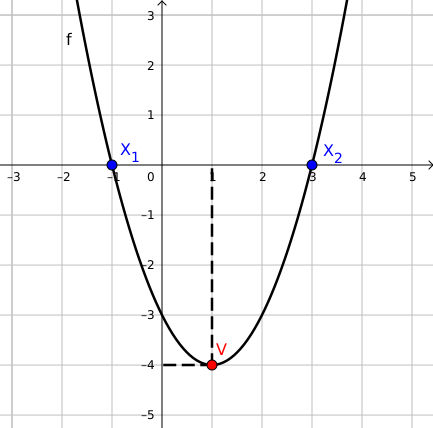
\includegraphics[width=7cm,height=5cm]{./cap_funcao/figs/funcao2grauexem1}}
   \caption{Gráfico da função $f(x)= x^2 - 2x - 3$}
  \end{figure}
\end{exem}

\begin{resol}
\begin{enumerate}
\item [a)] Os zeros de $f$ são $S= \{-1, 3\}$.
\item [b)] O vértice de $f$ é o ponto $V= (1, -4)$.
\item [c)] Esta função tem concavidade para cima.
\item [d)] O vértice desta função é ponto de mínimo.
\item [e)] A função é crescente no intervalo $(1, \infty)$.
\item [f)] A função é decrescente no intervalo $(- \infty, 1)$.
\end{enumerate}
\end{resol}

\begin{exem}
Considere a função $f(x)= -x^2 + 2x + 8$, determine:
\begin{enumerate}
\item [a)] Os zeros de $f$.
\item [b)] O vértice de $f$.
\item [c)] Esta função tem concavidade para cima ou para baixo?
\item [d)] O vértice desta função é ponto de máximo ou mínimo?
\item [e)] Qual o intervalo no qual a função é crescente?
\item [f)] Qual o intervalo no qual a função é decrescente?
\end{enumerate}
  \begin{figure}[H]
  \centering
  \fbox{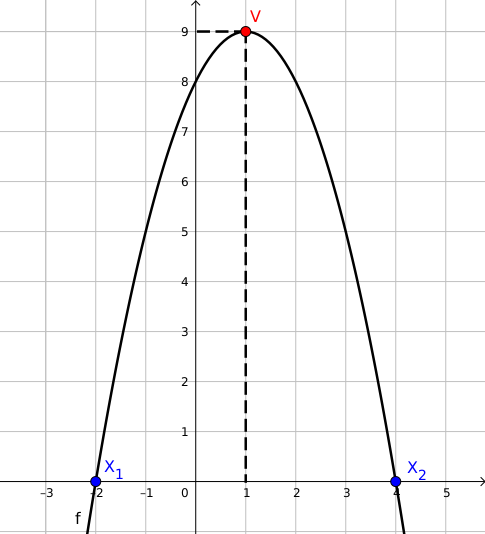
\includegraphics[width=7cm,height=6cm]{./cap_funcao/figs/funcao2grauexem2}}
   \caption{Gráfico da função $f(x)= -x^2 + 2x + 8$}
  \end{figure}
\end{exem}

\begin{resol}
\begin{enumerate}
\item [a)] Os zeros de $f$ são $S= \{-2, 4\}$.
\item [b)] O vértice de $f$ é o ponto $V= (1,9)$.
\item [c)] Esta função tem concavidade voltada para baixo.
\item [d)] O vértice desta função é ponto de máximo.
\item [e)] A função é crescente no intervalo $(-\infty, 1)$.
\item [f)] A função é decrescente no intervalo $(1, \infty)$.
\end{enumerate}
\end{resol}

 \section{Funções do 3º grau}
 As funções do 3º grau ou funções cúbicas são funções $f: \R \rightarrow \R$ dadas por:
\begin{equation}
f(x)= ax^3 + bx^2 + cx + d \ ,
\end{equation}

  para certos $a, b, c, d \in \R$ com $a \neq 0$. As \textbf{raízes} ou \textbf{zeros} das funções de 3º grau são os $x \in \R$ tais que $ax^3 + bx^2 + cx + d=0$. Assim as funções de 3º grau podem classificadas de acordo com suas raízes em 4 casos:
 \begin{enumerate}[(I)]
  \item 3 raízes reais distintas;
  \item 1 raiz real e duas raízes complexas;
  \item 3 raízes reais sendo duas delas iguais;
  \item 3 raízes reais iguais.
 \end{enumerate}
 Estes casos estão representados nos gráficos abaixo, onde consideramos sempre $a< 0$, o caso $a> 0$ é análogo.


   \begin{figure}[H]
   \fbox{\subfigure[$a < 0$]{\includegraphics[width=7cm,height=5cm]{./cap_funcao/figs/g1}}}
   \fbox{\subfigure[$a < 0$]{\includegraphics[width=7cm,height=5cm]{./cap_funcao/figs/g2}}}
   \end{figure}

  \begin{figure}[H]
   \fbox{\subfigure[$a < 0$]{\includegraphics[width=7cm,height=5cm]{./cap_funcao/figs/g3}}}
   \fbox{\subfigure[$a < 0$]{\includegraphics[width=7cm,height=5cm]{./cap_funcao/figs/g4}}}
   \caption{Gráficos de funções do 3º grau}
  \end{figure}
  


\section{Funções polinomiais de grau \texorpdfstring{$n$}{n}}

 \vskip0.3cm
 \colorbox{azul}{
 \begin{minipage}{0.9\linewidth}
 \begin{center}
 As funções $f: \R \to \R$ com a seguinte regra geral:
\begin{equation}
f(x) = a_0 + a_1 x + a_2 x^2 + a_3 x^3 + \cdots + a_n x^n
\end{equation}
 para $\{a_0, a_1, a_2, a_3, \ldots a_n\} \in \R$ e $n \in \N$, tais que $a_n \neq 0$ são denominadas \\ \textbf{funções polinomiais de grau $n$}.
 \end{center}
 \end{minipage}}
 \vskip0.3cm

Observe que as funções de 1ª, 2ª e 3ª grau são exemplos de funções polinomiais.

\section{Função definida por partes}

\begin{defi}
Uma função $f: A \to \R$, para $A \subset \R$, é dita ser definida por partes, quando particionamos o domínio $A$ em subconjuntos $U_i$ tais que $A= \bigcup_{i}U_i$, e para cada $U_i$ a função é dada por uma regra diferente. 
\end{defi}

\begin{exem}
\begin{equation}
f(x) = \begin{cases}
                 3x + 4, \text{ se } x < 2 \\
                 7 , \text{ se } x = 2 \\
                 -x^2 + 8, \text{ se } x > 2
                \end{cases} \ .
\end{equation}
   \begin{figure}[H]
  \centering
  \fbox{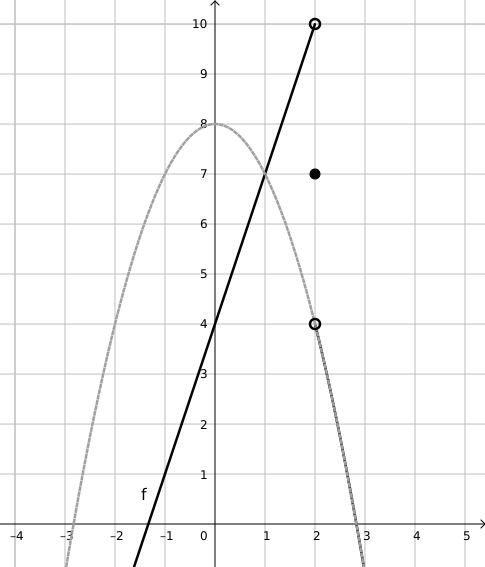
\includegraphics[width=7cm,height=6cm]{./cap_funcao/figs/funcaoPartesexem1}}
   \caption{Gráfico da função $f$}
  \end{figure}
\end{exem}

\begin{exem}
\begin{equation}
f(x) = \begin{cases}
                 -x^2 + 1, \text{ se } x < 0 \\
                 e^x, \text{ se } x \geqslant 0
                \end{cases} \ .
\end{equation}
   \begin{figure}[H]
  \centering
  \fbox{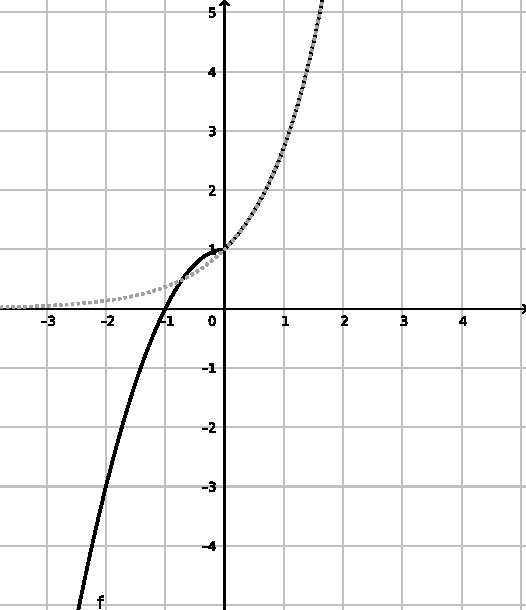
\includegraphics[width=7cm,height=6cm]{./cap_funcao/figs/funcaoPartesexem2}}
   \caption{Gráfico da função $f$}
  \end{figure}
\end{exem}

\begin{exem}
\begin{equation}
f(x) = \begin{cases}
                 -x + 1, \text{ se } x \leqslant 1 \\
                 ln(x), \text{ se } x > 1
                \end{cases} \ .
\end{equation}
\begin{figure}[H]
  \centering
  \fbox{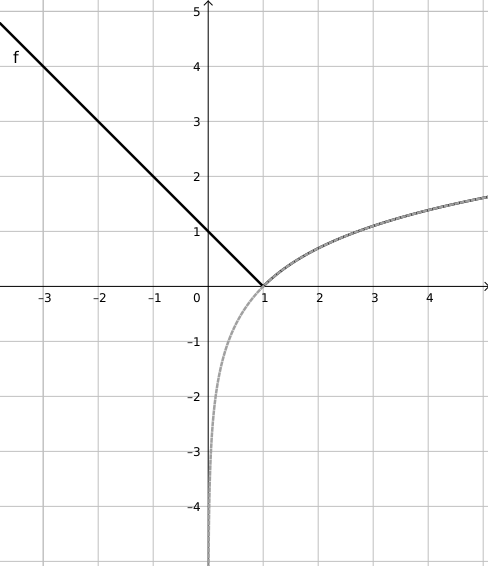
\includegraphics[width=7cm,height=6cm]{./cap_funcao/figs/funcaoPartesexem3}}
   \caption{Gráfico da função $f$}
  \end{figure}
\end{exem}

\begin{exem}
\begin{equation}
f(x) = \begin{cases}
                 x^2+2x+1, \text{ se } x < 1 \\
                 5, \text{ se } x = 1 \\
                -x+5, \text{ se } x > 1
                \end{cases} \ .
\end{equation}
\begin{figure}[H]
  \centering
  \fbox{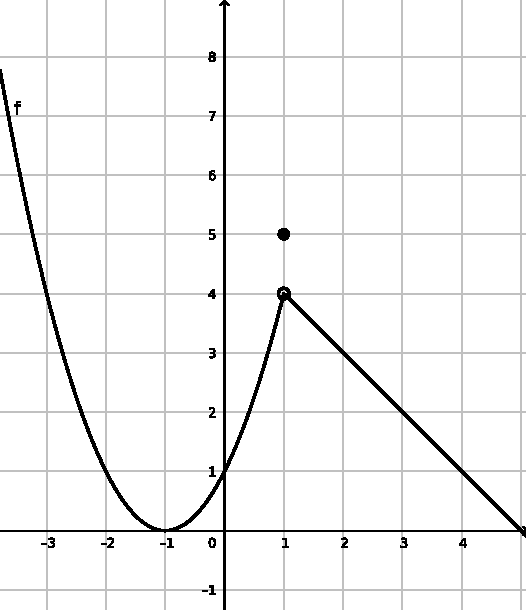
\includegraphics[width=7cm,height=7cm]{./cap_funcao/figs/funcaoPartesexem4}}
   \caption{Gráfico da função $f$}
  \end{figure}
\end{exem}

\section{Função modular}

  Considere a função $f: \R \rightarrow \R$, dada por $f(x)= \abs{x}$, pela definição de módulo temos que $f$ é uma função definida por partes, da seguinte forma:

  \[f(x)= \abs{x} = \begin{cases}
                 x, \text{ se } x \geq 0 \\
                 -x, \text{ se } x < 0
                \end{cases} \ .\]

 Cujo gráfico é dado por:

  \begin{figure}[H]
 \centering
    \fbox{\includegraphics[width=7cm]{./cap_funcao/figs/funcaomodulo}}
    \caption{Gráfico da função módulo}
  \end{figure}

Note que, $Im(f)= [0, \infty)$ e não todo o contradomínio que no caso é o conjunto $\R$. Além disso esta é uma função na qual as duas partes são lineares.
  
 \begin{exem}
 Vamos determinar os intervalos de crescimento e decrescimento, caso existam, da função $f(x)= \abs{x}$. Lembramos que esta função é definida por partes, por isso faremos a análise em cada uma destas partes.

  Caso 1: Se $x < 0$, temos que $f(x)= -x$, logo se $x_1 < x_2$,
\begin{equation}
x_1 < x_2 \Rightarrow -x_1 > -x_2 \Rightarrow f(x_1) > f(x_2) \ ,
\end{equation}
  por exemplo, sendo $x_1= -3$ e $x_2= -2$ temos que $x_1 < x_2$,
\begin{equation}
f(x_1)= f(-3)= -(-3)= 3 > 2= -(-2)= f(-2)= f(x_2) \ .
\end{equation}

  Portanto se $x < 0$ temos que $f$ é decrescente.

  Caso 2: Se $x \geq 0$, temos que $f(x)= x$, logo se $x_1 < x_2$
\begin{equation}
x_1 < x_2 \Rightarrow  f(x_1) < f(x_2) \ ,
\end{equation}
  por exemplo, sendo $x_1= 2$ e $x_2= 3$ temos que $x_1 < x_2$,
\begin{equation}
f(x_1)= 2 > 3= f(x_2) \ .
\end{equation}

  Portanto se $x \geq 0$ temos que $f$ é crescente.
 \end{exem}

\begin{exem}
  Consideramos agora a função $f_1: \R \rightarrow \R$ dada por $f_1(x)= \abs{x+1}$, observe que:
\begin{equation}
x+1 \geq 0 \Leftrightarrow  x \geq -1
\end{equation}
  com isso podemos reescrever a função $f_1$ sem os módulos da seguinte forma:

  \[f_1(x)= \begin{cases}
                 x + 1, \text{ se } x \geq -1 \\
                 -x - 1, \text{ se } x < -1
                \end{cases} \ .\]
  Com isso a função modular pode ser vista como uma função linear por partes.
\end{exem}

\begin{exem}
  Analogamente, para a função $f_2: \R \rightarrow \R$ dada por $f_2(x)= \abs{x+1}+2$, temos que:
\begin{equation}
x+1 \geq 0 \Leftrightarrow  x \geq -1
\end{equation}
  com isso podemos reescrever a função $f_2$ sem os módulos da seguinte forma:

  \[f_2(x)= \begin{cases}
                 x + 3, \text{ se } x \geq -1 \\
                 -x + 1, \text{ se } x < -1
                \end{cases} \ .\]
  Com isso a função modular também pode ser vista como uma função linear por partes.
\end{exem}

Os gráficos das funções $f$, $f_1$ e $f_2$ estão dados na figura a seguir.

  \begin{figure}[H]
 \centering
    \fbox{\includegraphics[width=8cm]{./cap_funcao/figs/funcaomodulo2}}
    \caption{Gráfico da função módulo}
  \end{figure}

  Comparando os gráficos das funções $f$ e $f_1$ notamos que ao somar uma constante ``dentro'' do módulo transladamos o gráfico da função $f$ no eixo $x$, e ao comparar as funções $f_1$ e $f_2$ percebemos que ao somar uma constante ``fora'' do módulo fazemos uma translação do gráfico da função $f_1$ em relação ao eixo $y$.
  
\section{Composição de funções}

\begin{defi}
Consideremos duas funções $f: A \rightarrow B$ e $g: B \rightarrow C$, com $A, B \text{ e } C \subset \R$, e note que $Im(f) \subset B$. A função composta $g \circ f: A \rightarrow C$ é definida por:
\begin{equation}
(g \circ f)(x)= g(f(x)). 
\end{equation}

 \begin{figure}[H]
 \centering
 \begin{tikzpicture}
 \centering
 \node (1) at (0,0) {1};%\filldraw(1.east) circle (1pt)
 \node (2) [below of=1] {2};%\filldraw(2.east) circle (1pt)
 \node (3) [below of=2] {3};%\filldraw(3.east) circle (1pt)
 \node[fit=(1) (2) (3),ellipse,draw=red,minimum width=1cm,thick,label=below:\(A\)]{};

 \node (a) at (3,0) {a};%\filldraw($b_1$.west) circle (1pt)
 \node (b) [below of=a] {b};%\filldraw($b_2$.west) circle (1pt)
 \node (c) [below of=b] {c};%\filldraw($b_3$.west) circle (1pt)
 \node (d) [below of=c] {d};%\filldraw($b_3$.west) circle (1pt)
 \node[fit=(a) (b) (c) (d),ellipse,draw=green,minimum width=1cm,thick,label=below:\(B\)]{};
 
 \node (A) at (6,0) {A};%\filldraw($b_1$.west) circle (1pt)
 \node (B) [below of=A] {B};%\filldraw($b_2$.west) circle (1pt)
 \node (C) [below of=B] {C};%\filldraw($b_3$.west) circle (1pt)
 \node (D) [below of=C] {D};%\filldraw($b_3$.west) circle (1pt)
 \node[fit=(A) (B) (C) (D),ellipse,draw=blue,minimum width=1cm,thick,label=below:\(C\)]{};

 \draw[->, shorten >=.1cm, >=stealth'] (1.east) to (b.west);
 \draw[->, shorten >=.1cm, >=stealth'] (2.east) to (c.west);
 \draw[->, shorten >=.1cm, >=stealth'] (3.east) to (a.west);
 
 \draw[->, shorten >=.1cm, >=stealth'] (a.east) to (A.west);
 \draw[->, shorten >=.1cm, >=stealth'] (b.east) to (B.west);
 \draw[->, shorten >=.1cm, >=stealth'] (c.east) to (C.west);
\end{tikzpicture}
\caption{Composição de funções}
\end{figure}

\end{defi}

Vejamos alguns exemplos de composições de função $\R \to \R$.

\begin{exem}
Com a função modular $f(x)= |x|$, e as funções lineares $g(x)= x+1$ e $h(x)= x-1$. Obtemos as seguintes funções compostas $\R \to \R$:
\begin{enumerate}
\item [a)] $(f \circ g)(x)= f(g(x)) \Rightarrow (f \circ g)(x)= |x+1|$;
\item [b)] $(f \circ h)(x)= f(h(x)) \Rightarrow (f \circ h)(x)= |x-1|$;
\item [c)] $(g \circ f)(x)= g(f(x)) \Rightarrow (g \circ f)(x)= |x|+1$;
\item [d)] $(h \circ f)(x)= h(f(x)) \Rightarrow (h \circ f)(x)= |x|-1$.
\end{enumerate}
Em cada um dos exemplos acima sugiro observar o movimento do gráfico no plano cartesiano.
\end{exem}

\begin{exem}
Considere a função modular $f(x)= |x|$, e a função quadrática $g(x)= x^2-x-6$. Temos as seguintes funções compostas $\R \to \R$:
\begin{enumerate}
\item [a)] $(f \circ g)(x)= f(g(x))= |x^2-x-6|$;
\item [b)] $(g \circ f)(x)= g(f(x))= |x|^2 - |x|- 6$.
\end{enumerate}
\end{exem}

\begin{exem}
Considerando a função linear $f(x)= -2x+4$, e a função quadrática $g(x)= x^2$. Chegamos as funções compostas 
\begin{enumerate}
\item [a)] $(f \circ g)(x)= f(g(x))= -2x^2 + 4$;
\item [b)] $(g \circ f)(x)= g(f(x))= (-2x+4)^2$.
\end{enumerate}
\end{exem}

\begin{exem}
Considere as funções reais:
\begin{eqnarray}
f(x)= -x^2 + 8x -7
\end{eqnarray}

\begin{eqnarray}
g(x)= \begin{cases}
       g_1(x)= |x|, \text{ se } x \leqslant 9 \\
       g_2(x)= x-3, \text{ se } x > 9
	  \end{cases}
\end{eqnarray}
Determine a função $(g \circ f)(x)= g(f(x))$.
\begin{resol}
Para fazer esta composição como a função $g$ é definida por partes precisamos qual é o conjunto imagem da função $f$. Note que $f$ é uma função do 2º grau com $a< 0$ logo concavidade voltada para baixo, o que nos diz que $Im(f)= (-\infty, y_v]$, por tanto basta calcular o $y_v$,
\begin{eqnarray}
y_v= \dfrac{- \Delta}{4a}= \dfrac{-(8^2-4.(-1).(-7))}{4.(-1)}= \dfrac{-36}{-4}= 9 \ .
\end{eqnarray}
Portanto, $Im(f)= (-\infty, 9]$. Assim, considerando a definição da função $g$, temos que
\begin{eqnarray}
(g \circ f)(x)= g(f(x))= g_1(f(x))= |-x^2 + 8x -7| \ .
\end{eqnarray}
\end{resol}
\end{exem}

\begin{exem}
Considere as funções reais:
\begin{eqnarray}
f(x)= \begin{cases}
      f_1(x)= -x^2+8x-7, \text{ se } x < 6 \\
      f_2(x)= x-1, \text{ se } x \geqslant 6
      \end{cases}
\end{eqnarray}

\begin{eqnarray}
g(x)= \begin{cases}
      g_1(x)= |x|, \text{ se } x < 5 \\
      g_2(x)= 2x-5, \text{ se } 5 \leqslant x \leqslant 9 \\
      g_3(x)= -x+22, \text{ se } x > 9
      \end{cases}
\end{eqnarray}
Determine a função $(g \circ f)(x)= g(f(x))$.

  \begin{figure}[H]
 \centering
    \fbox{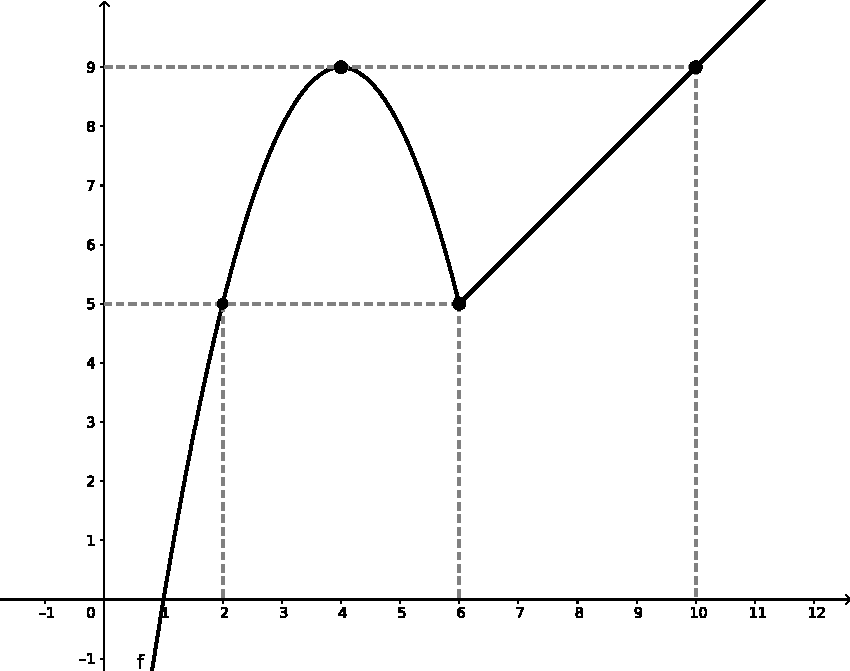
\includegraphics[width=8cm]{./cap_funcao/figs/funcaoCompostaexem5}}
    \caption{Gráfico da função $f$}
  \end{figure}

\begin{resol}
Como a função $g$ está definida por partes, para fazer a composição precisamos entender o comportamento do conjunto imagem da função $f$. Observamos que:
\begin{eqnarray}
\begin{cases}
f_1: (-\infty, 6) \to (-\infty, 9) \\
f_2: [6, \infty) \to [5, \infty) \ .
\end{cases}
\end{eqnarray}
 Com isso vemos que 
 \begin{eqnarray}
(g \circ f)(x)= \begin{cases}
      g_1(f_1(x))= |-x^2+8x-7|, \text{ se } x < 2 \\
      g_2(f_1(x))= 2*(-x^2+8x-7), \text{ se } 2 \leqslant x < 6 \\
      g_2(f_2(x))= 2*(x-1)-5, \text{ se } 6 \leqslant x \leqslant 10 \\
      g_3(f_2(x))= -(x-1)+22, \text{ se } x > 10
      \end{cases}
\end{eqnarray}
\end{resol}
\end{exem}

\begin{exem}
Considere as funções reais:
\begin{eqnarray}
f: [0, 2\pi] \to [-1, 1] \\
f(x)= sen(x)
\end{eqnarray}

\begin{eqnarray}
g(x)= \begin{cases}
      g_1(x)= -2x, \text{ se } x < -1 \\
      g_2(x)= 2|x|, \text{ se } -1 \leqslant x < 0 \\
      g_3(x)= 4x, \text{ se } 0 \leqslant x \leqslant 1 \\
      g_4(x)= x^2 + 3, \text{ se } x > 1
      \end{cases}
\end{eqnarray}
Determine a função $(g \circ f)(x)= g(f(x))$.

\begin{resol}
Sabemos que $Im(f)= [-1, 1]$, logo
\begin{eqnarray}
g(f(x))= \begin{cases}
      g_2(f(x))= 2|sen(x)|, \text{ se } \pi \leqslant x < 2\pi \\
      g_3(f(x))= 4*sen(x), \text{ se }  0 \leqslant x \leqslant \pi \\
      \end{cases}
\end{eqnarray}
  \begin{figure}[H]
 \centering
    \fbox{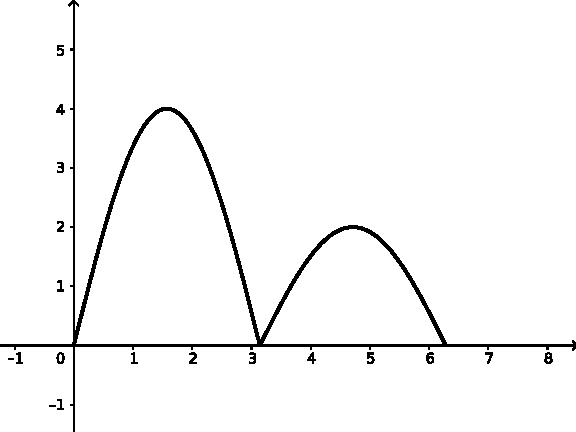
\includegraphics[width=8cm]{./cap_funcao/figs/funcaoCompostaexem6}}
    \caption{Gráfico da função $(g \circ f)(x)$}
  \end{figure}
\end{resol}
\end{exem}

\begin{exem}
As funções:
\begin{itemize}
\item $h_1: \R \setminus \{k*\pi \mid k \in \Z\} \to \R$ dada por $h_1(x)= \dfrac{1}{sen(x)}$;
  \begin{figure}[H]
 \centering
    \fbox{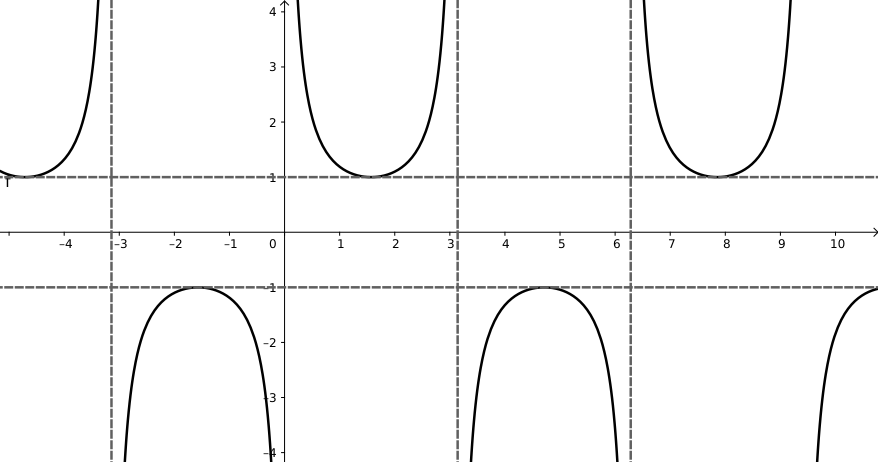
\includegraphics[width=8cm]{./cap_funcao/figs/funcaoCompostaexem7h1}}
    \caption{Gráfico da função $h_1(x)$}
  \end{figure}
\item $h_2: \R \setminus \{0\} \to \R$ dada por $h_2(x)= sen \left(\dfrac{1}{x} \right)$
  \begin{figure}[H]
 \centering
    \fbox{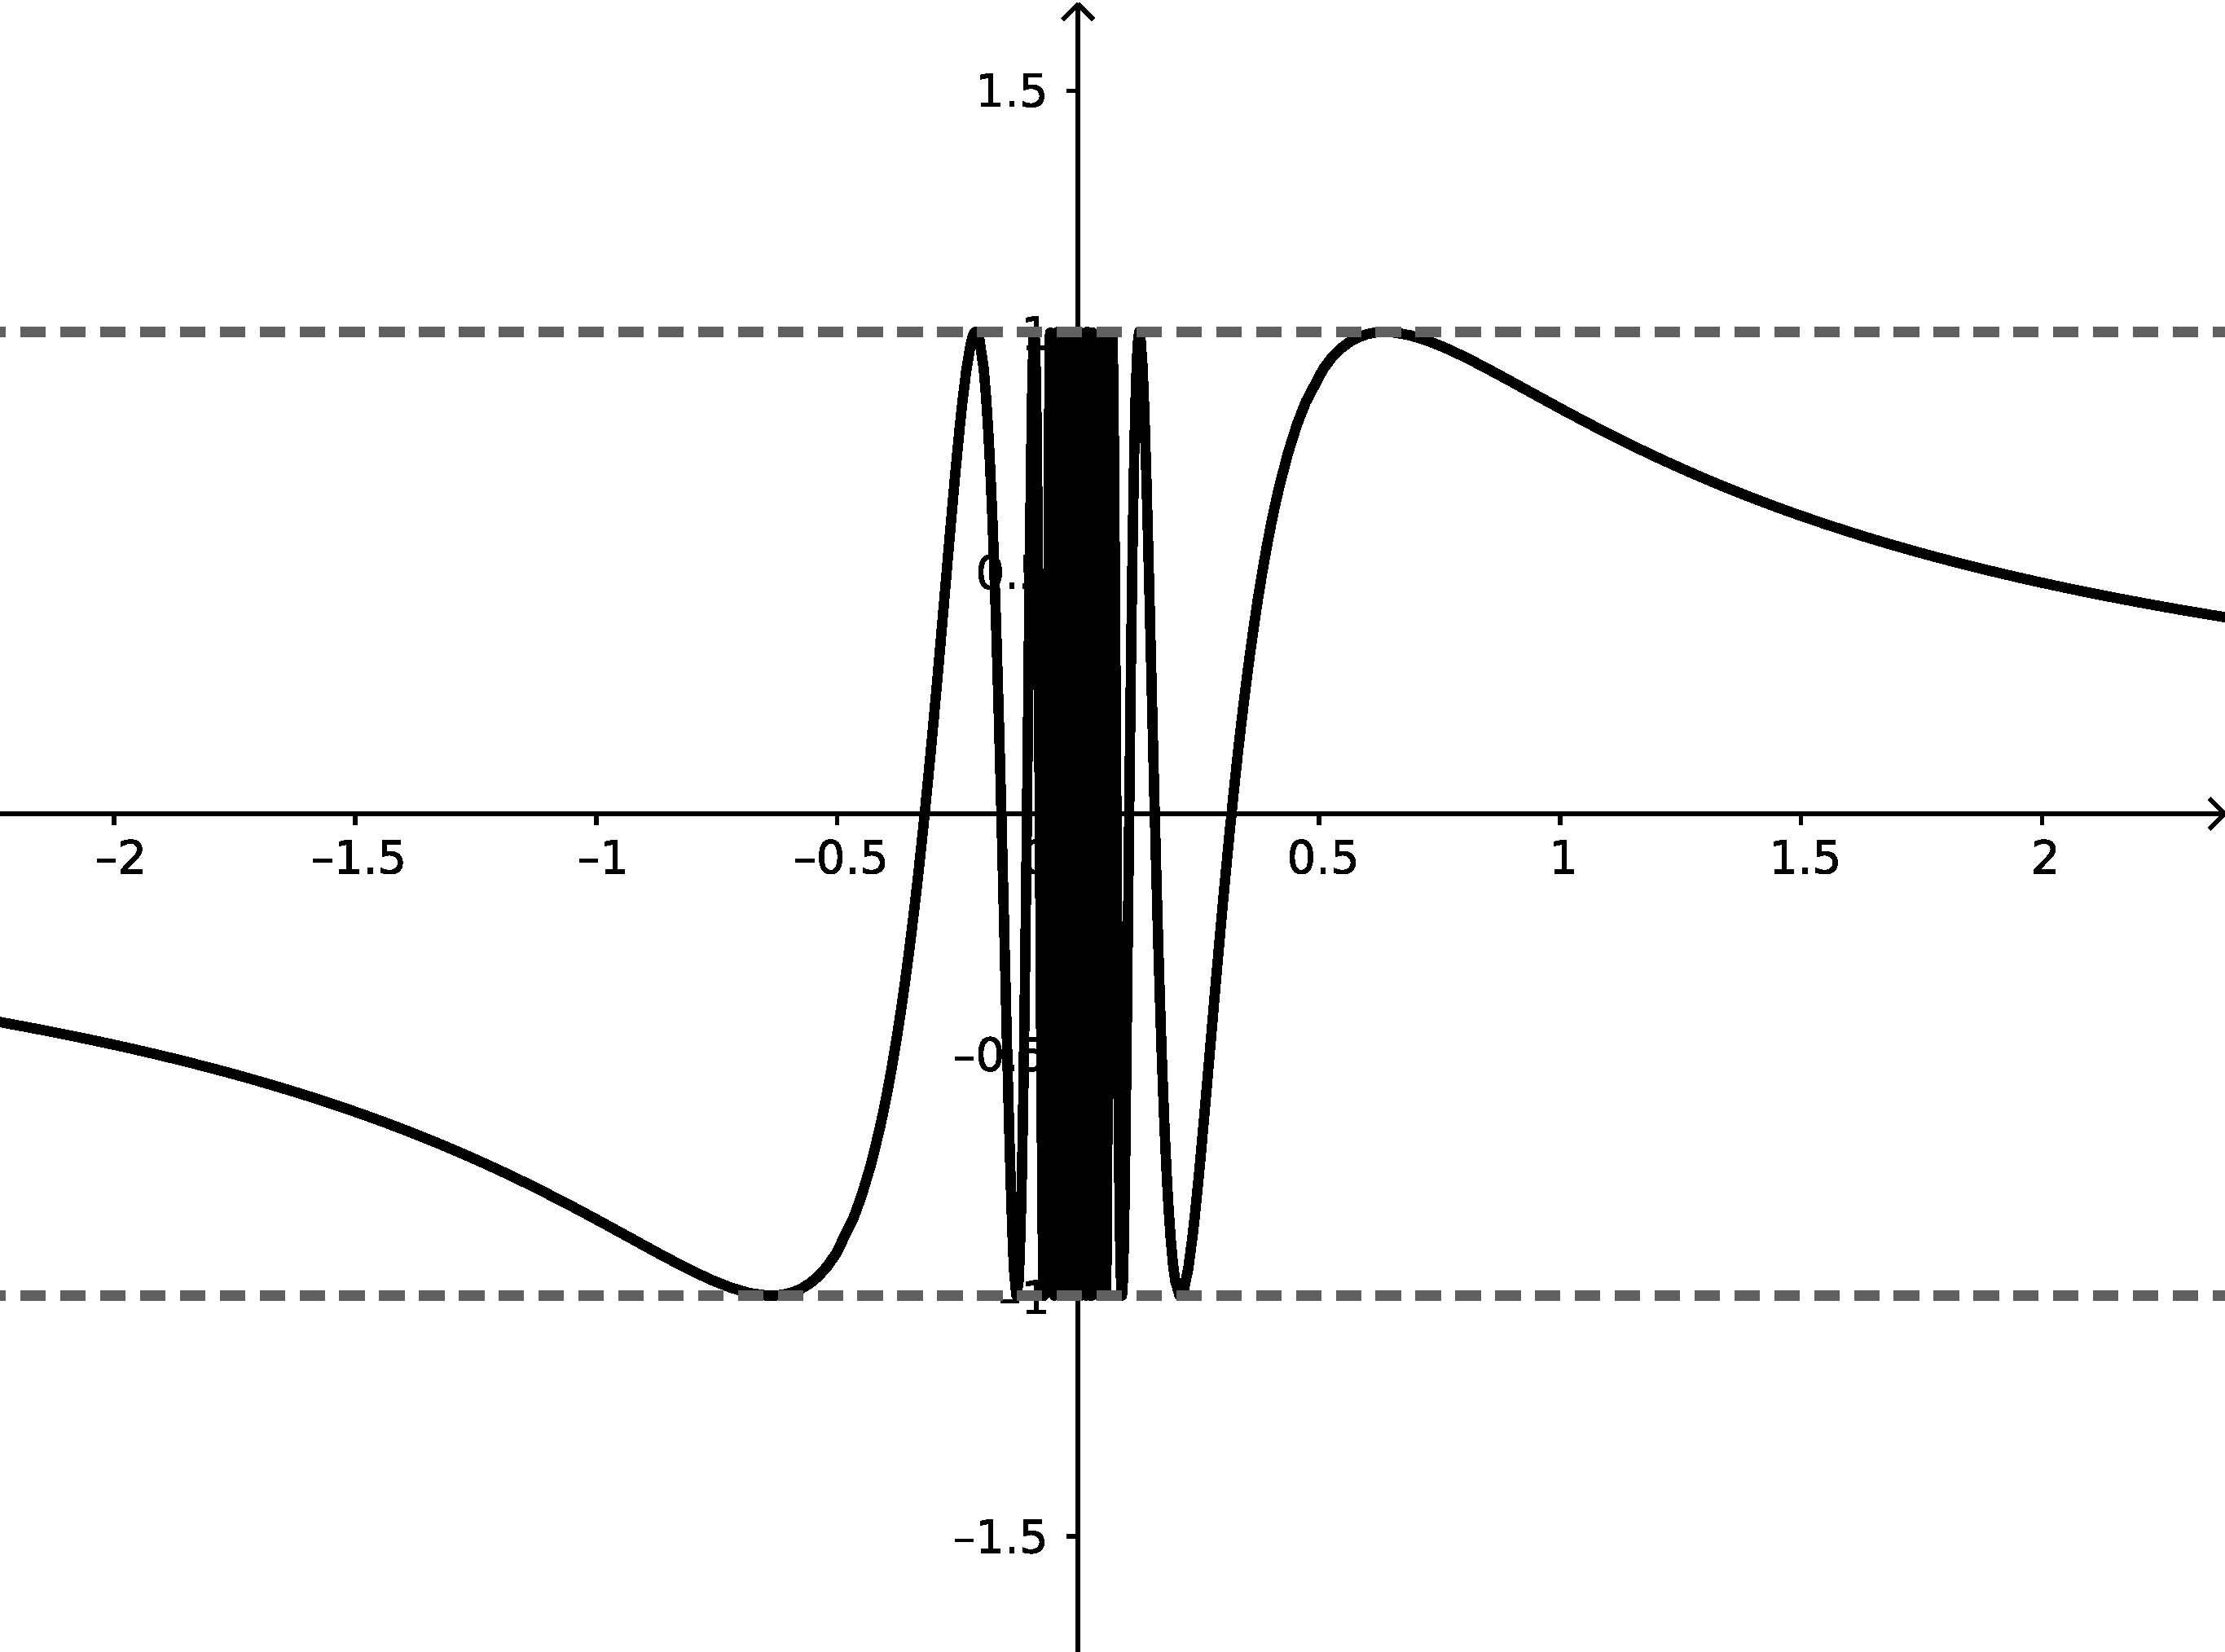
\includegraphics[width=8cm]{./cap_funcao/figs/funcaoCompostaexem7h2}}
    \caption{Gráfico da função $h_2(x)$}
  \end{figure}
\end{itemize}
podem ser entendidas como composição das funções $f(x)= sen(x)$ e $g(x)= \dfrac{1}{x}$, com as devidas restrições nos conjuntos domínio. Observe que $h_1(x)= g(f(x))$ e $h_2(x)= f(g(x))$.
\end{exem}



\section{Algumas funções interessantes}

  \textbf{Função raiz quadrada}

  É a função $f: \R_{+} \to \R_{+}$ dada por $f(x)= \sqrt{x}$, cujo gráfico é:

   \begin{figure}[H]
 \centering
    \fbox{\includegraphics[width=6cm]{./cap_funcao/figs/funcaoraizquadrada}}
    \caption{Função raiz quadrada}
  \end{figure}

  Note que neste caso o domínio da função são apenas os números reais positivos, já que não existe raiz quadrada de número negativo.

  \textbf{Função raiz cúbica}

  É a função $f: \R \to \R$ dada por $f(x)= \sqrt[3]{x}$, cujo gráfico é:

   \begin{figure}[H]
 \centering
    \fbox{\includegraphics[width=6cm]{./cap_funcao/figs/funcaoraizcubica}}
    \caption{Função raiz cúbica}
  \end{figure}

  \textbf{Função recíproca}

  É a função $f: \R \setminus \{0\} \to \R$ dada por $f(x)= \frac{1}{x}$, cujo gráfico é:

   \begin{figure}[H]
 \centering
    \fbox{\includegraphics[width=6cm]{./cap_funcao/figs/funcaoreciproca}}
    \caption{Função recíproca}
  \end{figure}

  Neste caso o domínio da função é o conjunto $\R \setminus \{0\}$, pois não existe divisão por $0$ (zero).



  \textbf{Função floor}

  É a função $f: \R \to \R$ dada por $f(x)= \lfloor {x} \rfloor$, cujo gráfico é:

   \begin{figure}[H]
 \centering
    \fbox{\includegraphics[width=6cm]{./cap_funcao/figs/funcaofloor}}
    \caption{Função floor}
  \end{figure}

  Esta função aplicada em um número $x$ tem como imagem a parte inteira do número $x$.

  \textbf{Função ceil}

  É a função $f: \R \to \R$ dada por $f(x)= \lceil {x} \rceil$, cujo gráfico é:

   \begin{figure}[H]
 \centering
    \fbox{\includegraphics[width=6cm]{./cap_funcao/figs/funcaoceil}}
    \caption{Função ceil}
  \end{figure}

  Esta função aplicada em um número $x$ tem como imagem o menor inteiro maior ou igual a $x$.

\newpage
\section{Funções injetoras e/ou sobrejetoras}

\begin{itemize}
 \item \textbf{Injetora}

 Uma função $f: A \rightarrow B$ é injetiva, ou injetora quando:
\begin{equation}
 x_1 \neq x_2 \in A \Rightarrow f(x_1) \neq f(x_2) \in B ,
\end{equation}
 ou equivalentemente usando a contrapositiva:
\begin{equation}
f(x_1) = f(x_2) \in B \Rightarrow x_1 = x_2 .
\end{equation}
 Ou seja, quando cada elemento da $Im(f)$ recebe um único elemento de $A= Dom(f)$, neste caso pode ocorrer de alguns elementos de $B$ não serem imagem de nenhum elemento de $A$ pela função $f$.

 \item \textbf{Sobrejetora}

 Uma função $f: A \rightarrow B$ é sobrejetiva, ou sobrejetora quando para todo $y \in B$, existe pelo menos um elemento $x \in A$ tal que $f(x) = y$. Equivalentemente em símbolos:
\begin{equation}
\forall y \in B, \exists x \in A \text{ tal que } f(x) = y
\end{equation}
 Ou ainda, quando cada elemento de $B$ recebe algum elemento de $A$, neste caso podendo não ser único.

 \item \textbf{Bijetora}

 Uma função $f: A \rightarrow B$ é bijetora, ou bijetiva quando for simultaneamente injetora e sobrejetora. Neste caso, $f$ admite uma inversa que é denotada por $f^{(-1)}$.

\end{itemize}

\begin{multicols}{2}
\begin{figure}[H]
\centering
 \begin{tikzpicture}
 \node (1) at (0,0) {1};%\filldraw(1.east) circle (1pt)
 \node (2) [below of=1] {2};%\filldraw(2.east) circle (1pt)
 \node (3) [below of=2] {3};%\filldraw(3.east) circle (1pt)
 \node[fit=(1) (2) (3),ellipse,draw=red,minimum width=1cm,thick,label=below:\(A\)]{};

 \node (a) at (3,0) {a};%\filldraw($b_1$.west) circle (1pt)
 \node (b) [below of=a] {b};%\filldraw($b_2$.west) circle (1pt)
 \node (c) [below of=b] {c};%\filldraw($b_3$.west) circle (1pt)
 \node[fit=(a) (b) (c),ellipse,draw=green,minimum width=1cm,thick,label=below:\(B\)]{};

 \draw[->, shorten >=.1cm, >=stealth'] (1.east) to (c.west);
 \draw[->, shorten >=.1cm, >=stealth'] (2.east) to (b.west);
 \draw[->, shorten >=.1cm, >=stealth'] (3.east) to (a.west);
\end{tikzpicture}
\caption{Função bijetora}
\end{figure}

\begin{figure}[H]
\centering
 \begin{tikzpicture}
 \node (1) at (0,0) {1};%\filldraw(1.east) circle (1pt)
 \node (2) [below of=1] {2};%\filldraw(2.east) circle (1pt)
 \node (3) [below of=2] {3};%\filldraw(3.east) circle (1pt)
 \node[fit=(1) (2) (3),ellipse,draw=red,minimum width=1cm,thick,label=below:\(A\)]{};

 \node (a) at (3,0) {a};%\filldraw($b_1$.west) circle (1pt)
 \node (b) [below of=a] {b};%\filldraw($b_2$.west) circle (1pt)
 \node[fit=(a) (b),ellipse,draw=green,minimum width=1cm,thick,label=below:\(B\)]{};

 \draw[->, shorten >=.1cm, >=stealth'] (1.east) to (a.west);
 \draw[->, shorten >=.1cm, >=stealth'] (2.east) to (a.west);
 \draw[->, shorten >=.1cm, >=stealth'] (3.east) to (b.west);
\end{tikzpicture}
\caption{Função sobrejetora e não injetora}
\end{figure}
\end{multicols}


\begin{multicols}{2}
\begin{figure}[H]
\centering
 \begin{tikzpicture}
 \node (1) at (0,0) {1};%\filldraw(1.east) circle (1pt)
 \node (2) [below of=1] {2};%\filldraw(2.east) circle (1pt)
 \node (3) [below of=2] {3};%\filldraw(3.east) circle (1pt)
 \node[fit=(1) (2) (3),ellipse,draw=red,minimum width=1cm,thick,label=below:\(A\)]{};

 \node (a) at (3,0) {a};%\filldraw($b_1$.west) circle (1pt)
 \node (b) [below of=a] {b};%\filldraw($b_2$.west) circle (1pt)
 \node (c) [below of=b] {c};%\filldraw($b_3$.west) circle (1pt)
 \node[fit=(a) (b) (c),ellipse,draw=green,minimum width=1cm,thick,label=below:\(B\)]{};

 \draw[->, shorten >=.1cm, >=stealth'] (1.east) to (b.west);
 \draw[->, shorten >=.1cm, >=stealth'] (2.east) to (b.west);
 \draw[->, shorten >=.1cm, >=stealth'] (3.east) to (a.west);
\end{tikzpicture}
\caption{Função não sobrejetora e não injetora}
\end{figure}

\begin{figure}[H]
\centering
 \begin{tikzpicture}
 \node (1) at (0,0) {1};%\filldraw(1.east) circle (1pt)
 \node (2) [below of=1] {2};%\filldraw(2.east) circle (1pt)
 \node (3) [below of=2] {3};%\filldraw(3.east) circle (1pt)
 \node[fit=(1) (2) (3),ellipse,draw=red,minimum width=1cm,thick,label=below:\(A\)]{};

 \node (a) at (3,0) {a};%\filldraw($b_1$.west) circle (1pt)
 \node (b) [below of=a] {b};%\filldraw($b_2$.west) circle (1pt)
 \node (c) [below of=b] {c};%\filldraw($b_3$.west) circle (1pt)
 \node (d) [below of=c] {d};%\filldraw($b_3$.west) circle (1pt)
 \node[fit=(a) (b) (c) (d),ellipse,draw=green,minimum width=1cm,thick,label=below:\(B\)]{};

 \draw[->, shorten >=.1cm, >=stealth'] (1.east) to (b.west);
 \draw[->, shorten >=.1cm, >=stealth'] (2.east) to (c.west);
 \draw[->, shorten >=.1cm, >=stealth'] (3.east) to (a.west);
\end{tikzpicture}
\caption{Função não sobrejetora e injetora}
\end{figure}
\end{multicols}

\begin{exem}

 \begin{enumerate}
  \item $f: \mathbb{R} \rightarrow \mathbb{R}$ tal que $f(x) = x^2$

  Neste caso, $f$ não é sobrejetora, nem injetora.

  \begin{dem}

   \begin{itemize}
    \item Sobrejetora

    $f$ não é sobrejetora porque $x^2 \geq 0$, $\forall x \in \mathbb{R}$, logo se considerarmos $y < 0 \in \mathbb{R}$ teremos que $\nexists x \in \mathbb{R}$ tal que $f(x)= y$. Portanto $f$ não é sobrejetora.
    \fim
    \item Injetora

     Note que $ \forall x \in \mathbb{R} \Rightarrow -x \in \mathbb{R}$ e que
\begin{equation}
f(-x)= (-x)^2 = (-x)*(-x) = (x)*(x) = x^2 = f(x)
\end{equation}
    o que mostra que $f$ não é injetora.

   \end{itemize}
  \end{dem}

  \item $f: \mathbb{R_{+}} \rightarrow \mathbb{R}$ tal que $f(x) = x^2$

  Neste caso, $f$ não é sobrejetora, mas é injetora.

  \begin{dem}
   \begin{itemize}
    \item Sobrejetora

    $f$ não é sobrejetora porque $x^2 \geq 0$, $\forall x \in \mathbb{R}$, logo se considerarmos $y < 0 \in \mathbb{R}$ teremos que $\nexists x \in \mathbb{R}$ tal que $f(x)= y$. Portanto $f$ não é sobrejetora.
    \fim
    \item Injetora

    Tome $x_1=x_2 \in \mathbb{R_{+}}$ qualquer, como
\begin{equation}
x_1=x_2 \Rightarrow x_1^2=x_2^2 \Rightarrow f(x_1)=f(x_2)
\end{equation}
    logo $f$ é injetora.

   \end{itemize}
  \end{dem}

  \item $f: \mathbb{R} \rightarrow \mathbb{R_{+}}$ tal que $f(x) = x^2$

  Neste caso, $f$ é sobrejetora, mas não é injetora.

  \begin{dem}
   \begin{itemize}
    \item Sobrejetora

    Tome $y \in \mathbb{R_{+}}$ qualquer, como $y \geq 0$ existe $x \in \mathbb{R}$ tal que
\begin{equation}
x = \sqrt{y} \Rightarrow x^2 = (\sqrt{y})^2 \Rightarrow x^2 = y \Rightarrow f(x) = y 
\end{equation}
    portanto $f$ é sobrejetora.
    \fim
    \item Injetora

    Note que $ \forall x \in \mathbb{R} \Rightarrow -x \in \mathbb{R}$ e que
\begin{equation}
f(-x)= (-x)^2 = (-x)*(-x) = (x)*(x) = x^2 = f(x)
\end{equation}
    o que mostra que $f$ não é injetora.

   \end{itemize}
  \end{dem}

  \item $f: \mathbb{R_{+}} \rightarrow \mathbb{R_{+}}$ tal que $f(x) = x^2$ ou $f: \mathbb{R_{-}} \rightarrow \mathbb{R_{+}}$ tal que $f(x) = x^2$

  Neste caso, $f$ é sobrejetora, e é injetora, portanto bijetora.

  \begin{dem}
   \begin{itemize}
    \item Sobrejetora

    Tome $y \in \mathbb{R_{+}}$ qualquer, como $y \geq 0$ existe $x \in \mathbb{R}$ tal que
\begin{equation}
x = \sqrt{y} \Rightarrow x^2 = (\sqrt{y})^2 \Rightarrow x^2 = y \Rightarrow f(x) = y
\end{equation}
    portanto $f$ é sobrejetora.
    \fim
    \item Injetora

    Tome $x_1, x_2 \in \R_{+}$, tais que $f(x_1) = f(x_2)$ logo,
\begin{equation}
f(x_1) = f(x_2) \Rightarrow x_1^2= x_2^2 \Rightarrow \sqrt{x_1^2}= \sqrt{x_2^2} \Rightarrow \abs{x_1}= \abs{x_2} \Rightarrow x_1= x_2, 
\end{equation}
    pois $x_1, x_2 \geqslant 0$. Portanto $f$ é injetora.

   \end{itemize}
  \end{dem}

 \end{enumerate}

\end{exem}

\subsection{Função inversa}

 Considere uma função $f: A \rightarrow B$, para $A, B \subset \R$. Se existir uma função $g: B \rightarrow A$ tal que:
 \[(g \circ f)(x)= x, \forall x \in A \ \ \ \text {e} \ \ \
 (f \circ g)(x)= x, \forall x \in B\]
 dizemos que $f$ é inversível e que $g$ é a inversa de $f$. Denotamos por $g= f^{-1}$.

 Ficamos com a seguinte pergunta: Quando existe $f^{-1}$? E a resposta é:

 \vskip0.3cm

 \colorbox{azul}{
 \begin{minipage}{0.9\linewidth}
 \begin{center}
 Uma função $f: A \to B$ é inversível se, e somente se, $f$ for bijetora, ou seja, injetora e sobrejetora.
 \end{center}
 \end{minipage}}

 \vskip0.3cm

\begin{exem}
 A função $f: \R \rightarrow \R$ dada por $f(x)= x+2$ é injetora, e sobrejetora portanto, existe uma função $g: \R \rightarrow \R$ dada por $g(x)= x-2$, tal que:
\begin{eqnarray}
(f \circ g)(x)&=& (x-2) + 2= x-2+2= x \\
\Rightarrow (f \circ g)(x)&=& Id(x)
\end{eqnarray}
e ainda,
\begin{eqnarray}
(g \circ f)(x)&=& (x+2) - 2= x+2-2= x \\
\Rightarrow (g \circ f)(x)&=& Id(x) ,
\end{eqnarray}
logo $g= f^{-1}$ é a função inversa de $f$.

 \begin{figure}[H]
 \centering
    \fbox{\includegraphics[width=8cm]{./cap_funcao/figs/funcao_composta}}
    \caption{Composta das funções $f$ e $g$}
  \end{figure}

\end{exem}


\section{Paridade de uma função}

 \vskip0.3cm
 \colorbox{azul}{
 \begin{minipage}{0.9\linewidth}
 \begin{center}
  Dada um função $f: \R \rightarrow \R$.

  Dizemos que $f$ é uma \textbf{função par} se, para todo $x \in R$,
\begin{equation}
f(-x)= f(x) \ .
\end{equation}
  Dizemos que $f$ é uma \textbf{função ímpar} se, para todo $x \in R$,
\begin{equation}
f(-x)= - f(x) \ .
\end{equation}
 \end{center}
 \end{minipage}}
 \vskip0.3cm


 \begin{exem}
  \begin{enumerate}[a)]
   \item A função $f(x)= x$ é uma função ímpar;
\begin{equation}
f(-x)= -x= -f(x) 
\end{equation}
   \item A função $f(x)= x^2$ é uma função par;
\begin{equation}
f(-x)= (-x)^2= x^2 = f(x) 
\end{equation}
   \item A função $f(x)= x^3$ é uma função ímpar.
\begin{equation}
f(-x)= (-x)^3= -x^3= -f(x)
\end{equation}
  \end{enumerate}
 \end{exem}

 \begin{exem}
  Vamos analisar a paridade de função modular $f(x)= \abs{x}$.

  Caso 1: Se $x < 0$,
\begin{equation}
f(x)= \abs{x}= -x= f(-(x))= f(-x)
\end{equation}
  por exemplo, $x= -2$, neste caso,
\begin{equation}
f(x)= f(-2)= \abs{-2}= -(-2)= 2= f(2)= f(-(-2))= f(-x) \ ;
\end{equation}

  Caso 2: Se $x \geq 0$,
\begin{equation}
f(x)= \abs{x}= x= -(-x)= \abs{-x}= f(-x)
\end{equation}
  por exemplo, $x= 2$, neste caso,
\begin{equation}
f(x)= f(2)= \abs{2}= 2= -(-2)= \abs{-2}= f(-2)= f(-x) \ .
\end{equation}

  Portanto $f$ é uma função par.
 \end{exem}


\newpage
 \section{Mudando os gráficos das funções}

 \subsection{Translação do gráfico das funções}

 Dados $A, B \subset \R$ e uma função $f(x): A \to B$, definimos a função translação de $f$ no eixo $y$, pela função $g(x): A \to B$, dada por \destaque{g(x)= f(x) + c}, onde $c \in \R$ é uma constante.

 \begin{exem}
  Considere a função $f(x): \R \to \R$, dada por $f(x)= x^2$. Defina as seguintes funções $g: \R \to \R$ dada por $g(x)= f(x) + 2= x^2 + 2$, e $h: \R \to \R$ dada por $h(x)= f(x) - 2= x^2 - 2$, observe na seguinte figura como estas translações alteram o gráfico da função $f$, note a função $g$ carregou o gráfico da $f$ duas unidades ``para cima'' no eixo $y$, já a função $h$ carregou o gráfico da $f$ duas unidades ``para baixo'' no eixo $y$.

 \begin{figure}[H]
   \fbox{\subfigure[Gráficos das funções $f$ e $g$]{\includegraphics[width=7cm,height=6cm]{./cap_funcao/figs/translacaomais2}}}
   \fbox{\subfigure[Gráficos das funções $f$ e $h$]{\includegraphics[width=7cm,height=6cm]{./cap_funcao/figs/translacaomenos2}}}
\caption{Translação no eixo $y$}
  \end{figure}

 \end{exem}

  Dados $A, B \subset \R$ e uma função $f(x): A \to B$, definimos a função translação de $f$ no eixo $x$, pela função $g(x): A \to B$, dada por \destaque{g(x)= f(x + c)}, onde $c \in \R$ é uma constante.

 \begin{exem}
  Considere a função $f(x): \R \to \R$, dada por $f(x)= x^2$. Defina as seguintes funções $g: \R \to \R$ dada por $g(x)= f(x + 2)= (x+2)^2$, e $h: \R \to \R$ dada por $h(x)= f(x-2)= (x-2)^2$, observe na seguinte figura como estas translações alteram o gráfico da função $f$, note a função $g$ carregou o gráfico da $f$ duas unidades ``para à esquerda'' no eixo $x$, já a função $h$ carregou o gráfico da $f$ duas unidades ``para à direita'' no eixo $x$.

 \begin{figure}[H]
   \fbox{\subfigure[Gráficos das funções $f$ e $g$]{\includegraphics[width=7cm,height=6cm]{./cap_funcao/figs/translacaoXmais2}}}
   \fbox{\subfigure[Gráficos das funções $f$ e $h$]{\includegraphics[width=7cm,height=6cm]{./cap_funcao/figs/translacaoXmenos2}}}
\caption{Translação no eixo $x$}
  \end{figure}

 \end{exem}

 \subsection{Reflexão do gráfico das funções}

 Dados $A, B \subset \R$ e uma função $f(x): A \to B$, definimos a função reflexão de $f$ no eixo $x$, pela função $g(x): A \to B$, dada por \destaque{g(x)= -f(x)}.

 \begin{exem}
  Considere a função $f(x): \R \to \R$, dada por $f(x)= x^2$. Defina a função $g: \R \to \R$ dada por $g(x)=-f(x)= -x^2$, note que $g$ é por definição a reflexão da função $f$ em torno do eixo $x$, como pode ser visto pela figura:

\begin{figure}[H]
   \centering
   \fbox{\includegraphics[width=7cm]{./cap_funcao/figs/reflexaoemX}}
   \caption{Reflexão no eixo $x$}
  \end{figure}

 \end{exem}


 Dados $A, B \subset \R$ e uma função $f(x): A \to B$, definimos a função reflexão de $f$ no eixo $y$, pela função $g(x): A \to B$, dada por \destaque{g(x)= f(-x)}.

 \begin{exem}
  Considere a função $f(x): \R \to \R$, dada por $f(x)= x^3$. Defina a função $g: \R \to \R$ dada por $g(x)=f(-x)= (-x)^3$, note que $g$ é por definição a reflexão da função $f$ em torno do eixo $y$, como pode ser visto pela figura:

\begin{figure}[H]
   \centering
   \fbox{\includegraphics[width=7cm]{./cap_funcao/figs/reflexaoemY}}
   \caption{Reflexão no eixo $y$}
  \end{figure}

 \end{exem}

 Resumindo, dados $A, B \subset \R$, uma função $f(x): A \to B$, e uma constante $c \in \R$ obtemos as seguintes funções $g: A \to B$:
  \begin{table}[H]
 \centering
 \begin{tabular}{|c|c|} \hline
 \rowcolor{cinza}
  Mudança & Função \\\hline
  Translação no eixo $y$ & $g(x)= f(x)+ c$ \\\hline
  Translação no eixo $y$ & $g(x)= f(x)- c$ \\\hline
  Translação no eixo $x$ & $g(x)= f(x+ c)$ \\\hline
  Translação no eixo $x$ & $g(x)= f(x- c)$ \\\hline
  Reflexão no eixo $x$ & $g(x)= -f(x)$ \\\hline
  Reflexão no eixo $y$ & $g(x)= f(-x)$ \\\hline
 \end{tabular}
\end{table}

 \section{Exercícios} 
 \begin{exer}
 Uma bolsa de valores tinha um preço de R\$ $42,00$ quando sofreu uma queda de R\$$2,50$ por dia, durante $5$ dias seguidos.
  \begin{enumerate}[a)]
  \item Qual é a função que representa a queda do valor dessa ação em função do dia?
  \item Represente, no plano cartesiano, os pontos correspondentes a esses $5$ dias e o segmento de reta que passa por esses pontos.
  \end{enumerate}
  \end{exer}
  \begin{resp}
    a) $f(x)= 42 - 2,50 x$; b) a cargo do leitor;
  \end{resp}
  
  \begin{exer}
  Um táxi, realizando uma corrida, cobra uma taxa fixa denominada bandeira de R\$$3,50$ e R\$$0,80$ por quilômetro rodado.
  Com base nesses dados, determine:
  \begin{enumerate}[a)]
  \item A função que representa o valor pago por uma corrida de $x$ quilômetros.
  \item Quantos quilômetros foram rodados se a conta foi de R\$ $17,10$.
  \end{enumerate}
  \end{exer}
  \begin{resp}
    a) $f(x)= 3,50 + 0,80 x$; b) $x= 17 Km$;
  \end{resp}
  
  \begin{exer}
  Para cercar um terreno, tem-se duas opções:
  1ª) Taxa de entrega no local R\$ $100,00$ e R\$$12,00$ o metro linear de cerca.
  2ª) Taxa de entrega no local R\$ $80,00$ e R\$ $15,00$ o metro linear de cerca.
  \begin{enumerate}[a)]
  \item Represente o custo de cada opção para $x$ metros de cerca.
  \item Qual das duas opções é mais vantajosa para $140$m de perímetro.
  \end{enumerate}
  \end{exer}
  \begin{resp}
    a) 1ª opção: $f(x)= 100 + 12x$, 2ª opção: $f(x)= 80+15x$; b) 1ª opção; 
  \end{resp}
  
  \begin{exer}
  No Brasil, o sistema de numeração de sapatos ou tênis é baseado na fórmula $N(p)= \frac{5p + 28}{4}$, que indica o valor aproximado do número do calçado $N$ em função do comprimento $p$, em centímetros do pé da pessoa. Determine o número do sapato ou tênis que uma pessoa deve comprar se, ao medir o comprimento de seu pé obteve:
  \begin{enumerate}[a)]
  \item $22,8$ cm
  \item $24$ cm
  \item $26,4$ cm
  \end{enumerate}
  \end{exer}
  \begin{resp}
    a) $35,5$; b) $37$; c) $40$;
  \end{resp}

    %Este trabalho está licenciado sob a Licença Creative Commons Atribuição-CompartilhaIgual 4.0 Internacional. Para ver uma cópia desta licença, visite https://creativecommons.org/licenses/by-sa/4.0/ ou envie uma carta para Creative Commons, PO Box 1866, Mountain View, CA 94042, USA.

\chapter{Trigonometria}
 Possivelmente seu primeiro contato com trigonometria, foi ao estudar a trigonometria no triângulo retângulo, neste caso definimos as funções trigonométricas como razões entre os lados do triângulo e estamos restringindo seu domínio aos ângulos entre $0 \degree$ e $90 \degree$.
 Quando a trigonometria aparece novamente nos currículos ela ressurge através do círculo trigonométrico, que no começo fica restrito a compreensão da primeira volta do círculo ou seja ângulos entre $0 \degree$ e $360 \degree$, para depois ainda sobre o círculo aumentar o domínio da função.
 Antes de estudarmos as funções trigonométricas com domínio real vamos relembrar como este conceito era abordado nestes dois contextos já conhecidos.
 
 \section{Triângulo retângulo}

  Considere o triângulo retângulo, (triângulo que possui um de seus ângulos internos medindo $90 \degree$), como na figura abaixo:
  \begin{figure}[H]
   \centering
   \fbox{\includegraphics[width=7cm]{./cap_trigon/figs/triangulo_retangulo}}
   \caption{Triângulo retângulo}
  \end{figure}
 para este triângulo temos que é válido o seguinte teorema:

 \vskip0.3cm

\colorbox{azul}{
 \begin{minipage}{0.9\linewidth}
 \begin{center}
 \textbf{Teorema de Pitágoras}
\begin{equation}
a^2= b^2 + c^2.
\end{equation}
 \end{center}
 \end{minipage}}

 \vskip0.3cm

 \textit{Nota histórica:} De acordo com Howard Eves, em seu livro: \textit{"Introdução à história da Matemática"}, acredita-se que Pitágoras nasceu por volta de 572 a.c. na ilha egéia de Samos, e apesar deste teorema levar seu nome, este resultado já era conhecido pelos babilônios dos tempos de Hamurabi, mais de um milênio antes, mas sua primeira demonstração geral pode ter sido dada por Pitágoras.
 
 Este é um resultado importante, já que com ele é possível encontrar o valor de um dos lados do triângulo, nos casos em que não temos todos os lados dados.

 Para este triângulo, as funções seno, cosseno e tangente são dadas pelas seguintes razões trigonométricas, nesta ordem:

 \vskip0.3cm

\colorbox{azul}{
 \begin{minipage}{0.9\linewidth}
 \begin{center}
 \textbf{Funções trigonométricas}
  \begin{eqnarray*}
   \sen(\alpha)= \frac{c}{a}= \frac{CO}{HI} \ ; \ \
   \cos(\alpha)= \frac{b}{a}= \frac{CA}{HI} \ ; \ \
   \tan(\alpha)= \frac{c}{b}= \frac{CO}{CA}.
 \end{eqnarray*}
 \end{center}
 \end{minipage}}

 \vskip0.3cm

 Como a soma dos ângulos internos de um triângulo é $180 \degree$, e estamos aqui tratando de um triângulo retângulo, decorre que neste caso $0 \degree \leqslant \alpha \leqslant 90 \degree$. 
 
 Destacamos aqui os valores do seno, cosseno e tangente dos \emph{ângulos notáveis} que são os mais conhecidos:

 \begin{table}[H]
 \centering
 \begin{tabular}{|c|c|c|c|c|c|} \hline
 \rowcolor{cinza}
               & $0 \degree$  & $30 \degree$  & $45 \degree$  & $60 \degree$ & $90 \degree$  \\\hline
  $\pmb{\sen}$ & $0$ &$\frac{1}{2}$ & $\frac{\sqrt{2}}{2}$ & $\frac{\sqrt{3}}{2}$ & $1$ \\\hline
  $\pmb{\cos}$ & $1$ & $\frac{\sqrt{3}}{2}$ & $\frac{\sqrt{2}}{2}$ & $\frac{1}{2}$ & $0$ \\\hline
  $\pmb{\tan}$ & $0$ & $\frac{\sqrt{3}}{3}$ & $1$ & $\sqrt{3}$ & $\nexists$ \\\hline
 \end{tabular}
\end{table}
 Na próxima seção veremos como utilizar estes valores para calcular seno, cosseno e tangente de ângulos maiores que $90 \degree$.

\section{Círculo trigonométrico}

 No plano cartesiano, consideremos um círculo de centro na origem e raio $1$, neste círculo representamos as imagens das funções trigonométricas aplicadas à  $0 \degree \leqslant \alpha \leqslant 360 \degree$. Como mostra a seguinte figura:
 \begin{figure}[H]
   \centering
   \fbox{\includegraphics[width=9cm]{./cap_trigon/figs/circulo_trigonometrico}}
   \caption{Círculo trigonométrico}
  \end{figure}

 No círculo trigonométrico acima, temos destacado o ângulo de $30 \degree$ formado pelo raio do círculo com o eixo $x$. A projeção ortogonal deste raio sobre o eixo $x$ determina um segmento cujo comprimento é o valor do $cos(30 \degree)$, sobre o eixo $y$ determina um segmento cujo comprimento é o valor do $sen(30 \degree)$, e sobre a reta tangente determina um segmento cujo comprimento é o valor da $tan(30 \degree)$. Podemos aqui trocar o ângulo de $30 \degree$ por qualquer outro valor e encontraremos os valores do cosseno, seno e tangente deste novo ângulo da mesma forma.
 
  A partir do círculo trigonométrico concluímos que:

  \begin{table}[H]
 \centering
 \begin{tabular}{|c|c|c|c|} \hline
 \rowcolor{cinza}
               &  $120\degree$  & $135\degree$  &  $150\degree$ \\\hline
  $\pmb{\sen}$ & $\sen(60\degree)$ &$\sen(45\degree)$ & $\sen(30\degree)$  \\\hline
  $\pmb{\cos}$ & $-\cos(60\degree)$ &$-\cos(45\degree)$ & $-\cos(30\degree)$  \\\hline
  $\pmb{\tan}$ & $-\tan(60\degree)$ &$-\tan(45\degree)$ & $-\tan(30\degree)$  \\\hline
 \end{tabular}
\end{table}

 \begin{table}[H]
 \centering
 \begin{tabular}{|c|c|c|c|} \hline
 \rowcolor{cinza}
                & $210\degree$ & $225\degree$  & $240\degree$  \\\hline
  $\pmb{\sen}$ &  $-\sen(30\degree)$ & $-\sen(45\degree)$ & $-\sen(60\degree)$  \\\hline
  $\pmb{\cos}$ &  $-\cos(30\degree)$ & $-\cos(45\degree)$ & $-\cos(60\degree)$  \\\hline
  $\pmb{\tan}$ &  $\tan(30\degree)$ & $\tan(45\degree)$ & $\tan(60\degree)$   \\\hline
 \end{tabular}
\end{table}

 \begin{table}[H]
 \centering
 \begin{tabular}{|c|c|c|c|} \hline
 \rowcolor{cinza}
               & $300\degree$ & $315\degree$ & $330\degree$ \\\hline
  $\pmb{\sen}$ & $\sen(60\degree)$ & $\sen(45\degree)$ & $\sen(30\degree)$ \\\hline
  $\pmb{\cos}$ & $\cos(60\degree)$ & $\cos(45\degree)$ & $\cos(30\degree)$  \\\hline
  $\pmb{\tan}$ & $-\tan(60\degree)$ & $-\tan(45\degree)$ & $-\tan(30\degree)$  \\\hline
 \end{tabular}
\end{table}


  Os ângulos podem também ser representados em radianos, respeitando a seguinte relação:
  \destaque{\pi \text{ radianos}= 180 \degree}

  Usando esta relação podemos transformar graus para radianos e radianos para graus, vamos ver dois exemplos:

  \begin{exem}
   Qual a medida em graus do ângulo que mede $\frac{\pi}{4} rad$?

   \underline{Resolução:}

   Sabemos que $\pi rad= 180\degree$, portanto usando a regra de 3 abaixo conseguimos encontrar o valor em graus deste ângulo:
   \begin{eqnarray*}
  \text{Graus} & & \text{Radianos} \\
   180 & = & \pi\\
  x & = & \frac{\pi}{4}
 \end{eqnarray*}
 usando a propriedade da proporcionalidade, ou seja, multiplicando cruzado temos:

 $180 \cdot \frac{\pi}{4}= \pi \cdot x \Rightarrow \pi \cdot x= \frac{180 \pi}{4} \Rightarrow x= \frac{45 \pi}{\pi} \Rightarrow x= 45\degree$.

 \fim
  \end{exem}

  \begin{exem}
   Qual a medida em radianos do ângulo que mede $30\degree$?

   \underline{Resolução:}

   Sabemos que $\pi rad= 180\degree$, portanto usando a regra de 3 abaixo conseguimos encontrar o valor em graus deste ângulo:
   \begin{eqnarray*}
  \text{Graus} & & \text{Radianos} \\
   180 & = & \pi\\
  30 & = & x
 \end{eqnarray*}
 usando a propriedade da proporcionalidade, ou seja, multiplicando cruzado temos:

 $180 \cdot x= \pi \cdot 30 \Rightarrow x= \frac{30 \pi}{180} \Rightarrow x= \frac{\pi}{6} rad$.

 \fim
  \end{exem}

 \newpage

 \section{Identidades trigonométricas}

 \textbf{Identidades de quociente}

\begin{equation}
\tan(x)= \dfrac{\sen(x)}{\cos(x)} \qquad \cotan(x)= \dfrac{\cos(x)}{\sen(x)}
\end{equation}

 \vskip0.5cm
 \textbf{Identidades recíprocas}

 \[\sec(x)= \dfrac{1}{\cos(x)} \qquad
   \csc(x)= \dfrac{1}{\sen(x)} \qquad
   \cotan(x)= \dfrac{1}{\tan(x)}\]

 \vskip0.5cm
 \textbf{Identidades pitagóricas}

 \[\sen^2(x) + \cos^2(x)= 1 \qquad
   \tan^2(x)+ 1= \sec^2(x) \qquad
   \cotan^2(x)+1=\cosec^2(x)\]

 \vskip0.5cm
 \textbf{Identidades associadas à paridade}

\begin{equation}
\sen(-x)= -\sen(x) \qquad \cos(-x)= \cos(x) \qquad \tan(-x)=-\tan(x)
\end{equation}

 \vskip0.5cm
 \textbf{Identidades de arcos complementares}

 \[\sen \left(\frac{\pi}{2} - x \right)= \cos(x) \qquad
   \cos \left(\frac{\pi}{2} - x \right)= \sen(x)\]

 \[\tan \left(\frac{\pi}{2} - x \right)= \cotan(x) \qquad
   \cotan \left(\frac{\pi}{2} - x \right)= \tan(x)\]

 \[\cosec \left(\frac{\pi}{2} - x \right)= \sec(x) \qquad
   \sec \left(\frac{\pi}{2} - x \right)= \cosec(x)\]


\vskip0.5cm
 \textbf{Fórmulas de adição e subtração}

 Seno
 \begin{eqnarray*}
  \sen(a+b)&=&\sen(a)\cdot \cos(b)+\sen(b)\cdot \cos(a) \\
  \sen(a-b)&=&\sen(a)\cdot \cos(b)-\sen(b)\cdot \cos(a)
 \end{eqnarray*}

 Cosseno
 \begin{eqnarray*}
  \cos(a+b)&=&\cos(a)\cdot \cos(b)-\sen(a)\cdot \sen(b) \\
  \cos(a-b)&=&\cos(a)\cdot \cos(b)+\sen(a)\cdot \sen(b)
 \end{eqnarray*}

 Tangente
 \begin{eqnarray*}
  \tan(a+b)&=& \frac{\tan(a)+\tan(b)}{1-\tan(a)\cdot \tan(b)} \\
  \tan(a-b)&=& \frac{\tan(a)-\tan(b)}{1-\tan(a)\cdot \tan(b)}
 \end{eqnarray*}
 
\section{Exercícios}
\begin{exer}
 Calcule o valor da tangente, quando existir, dos seguintes ângulos:
 \begin{enumerate}[a)]
 \item $450\degree$
 \item $150\degree$
 \item $480\degree$
 \item $240\degree$
 \item $270\degree$
 \item $945\degree$
 \item $315\degree$
 \item $690\degree$
 \end{enumerate}
 \end{exer}
\begin{resp}
  \construirResp
\end{resp}
  
 
 \begin{exer}
 Dado o ângulo $\alpha= 50\degree$, sabendo que $sen(50\degree)= 0,766$. Determine:
 \begin{enumerate}[a)]
 \item O valor do $cos(\alpha)$.
 \item O valor da $tan(\alpha)$.
 \end{enumerate}
 \end{exer}
\begin{resp}
  \construirResp
\end{resp}

 \begin{exer}
 Dado o ângulo $\alpha= 140\degree$, sabendo que $sen(140\degree)= 0,76428$. Determine:
 \begin{enumerate}[a)]
 \item O valor do $cos(\alpha)$.
 \item O valor da $tan(\alpha)$.
 \end{enumerate}
 \end{exer}
\begin{resp}
  \construirResp
\end{resp}
 
 \begin{exer}
 Dado um triângulo retângulo contento um ângulo $\alpha$, com cateto adjacente a este ângulo sendo $c= 5 cm$ e a hipotenusa do triângulo sendo $a= 8,72 cm$. Determine:
 \begin{enumerate}[a)]
 \item O valor do $cos(\alpha)$.
 \item O valor do $sen(\alpha)$.
 \item O valor da $tan(\alpha)$.
 \end{enumerate}
 \end{exer}
\begin{resp}
  \construirResp
\end{resp}

 \begin{exer}
 Dado um triângulo retângulo contento um ângulo $\alpha$, com cateto oposto a este ângulo sendo $c= 5 cm$ e $sen(\alpha)= 0,7771$. Determine:
 \begin{enumerate}[a)]
 \item O valor do $cos(\alpha)$.
 \item O valor da $tan(\alpha)$.
 \end{enumerate}
 \end{exer}
\begin{resp}
  \construirResp
\end{resp}

 \begin{exer}
 Dado o ângulo $\alpha= 200\degree$, sabendo que $cos(200\degree)= -0,9397$. Determine:
 \begin{enumerate}[a)]
 \item O valor do $sen(\alpha)$.
 \item O valor da $tan(\alpha)$.
 \end{enumerate}
 \end{exer}
\begin{resp}
  \construirResp
\end{resp}

 \begin{exer}
 Dado o ângulo $\alpha= 350\degree$, sabendo que $sen(350\degree)= -0,1736$. Determine:
 \begin{enumerate}[a)]
 \item O valor do $cos(\alpha)$.
 \item O valor da $tan(\alpha)$.
 \end{enumerate}
 \end{exer}
\begin{resp}
  \construirResp
\end{resp}

 \begin{exer}
 Uma escada que mede $5m$ está apoiada em uma parede. Sabendo-se que ela forma com a parede um ângulo $\beta$ e que
\begin{equation}
sen(\beta)=\frac{\sqrt{7}}{3}.
\end{equation}
Qual é a distância de seu ponto de apoio no solo até a parede?
 \end{exer}
\begin{resp}
  \construirResp
\end{resp}

 \begin{exer}
 Quando o Sol se encontra a $60\degree$ acima do horizonte, uma árvore projeta sua sombra no chão com o comprimento de $8 m$. Determine a altura dessa árvore:
 \end{exer}
\begin{resp}
  \construirResp
\end{resp}

 \begin{exer}
 Quando o Sol se encontra a $45\degree$ acima do horizonte, um poste de iluminação projeta sua sombra no chão com o comprimento de $12 m$. Determine a altura desse poste:
 \end{exer}
\begin{resp}
  \construirResp
\end{resp}

 \begin{exer}
 De acordo com o comandante e consultor técnico da ABEAR, Paulo Roberto Alonso, “o avião parte do solo em um ângulo de 15 graus, medida essa que vai reduzindo durante a subida”. Para facilitar nosso cálculos suponhamos que esta medida não se altere. Supondo que a região sobrevoada pelo avião seja plana, qual será a altura atingida pelo avião depois de percorrer $900 m$?
 \end{exer}
\begin{resp}
  \construirResp
\end{resp}

 \begin{exer}
 Uma menina de $1,5m$ de altura avista o ponto mais alto de um morro, a partir de um ângulo de $20\degree$. Considerando que ela está a uma distância de $300m$ da base do morro, calcule a altura $(h)$ deste ponto.
 \end{exer}
\begin{resp}
  \construirResp
\end{resp}


\chapter{Funções trigonométricas}
   
 Vamos agora definir as funções trigonométricas no maior subconjunto real possível, e estudar o comportamento de seus gráficos. Mas para que este estudo seja completo precisamos antes definir os conceitos de período e amplitudade que são particularmente utéis para a compreenssão das funções trigonométricas.
 
  Estas funções fazem parte do grupo de funções periódicas, que são as funções que satisfazem a seguinte definição.

  \begin{defi}
   Uma função $f: \R \rightarrow \R$ é denominada \emph{periódica} quando existe um número real positivo $P$ tal que
\begin{equation}
f(x + P)= f(x)
\end{equation}
   para todo $x$ no domínio da $f$. O menor número real positivo $P$ que satisfaz esta propriedade é denominado período de $f$.
  \end{defi}
  
  Assim para entender seu comportamento em $\R$ basta conhecer como ela se comporta em um período.
  
  Além de periódica algumas funções trigonométricas são limitadas, ou seja admitem um valor máximo e um valor mínimo, e para estas funções podemos definir o conceito de amplitude como segue.
  
  \begin{defi}
  A \emph{amplitude} de oscilação $A$ de uma função limitada é dada por
  \begin{equation}
  A= \frac{y_{max} - y_{min}}{2} .
  \end{equation}
  \end{defi}
  
  De posse deste conceitos passamos agora para a definição das funções trigonométricas.
  
  \begin{itemize}
  \item Função Seno: $f: \R \rightarrow [-1, 1]$ dada por $f(x)= \sen (x)$, cujo gráfico é:

  \begin{figure}[H]
  \centering
    \fbox{\includegraphics[width=10cm]{./cap_trigon/figs/sen}}
    \caption{Gráfico da função $f(x)= \sen(x)$}
  \end{figure}

  \item Função Cosseno: $f: \R \rightarrow [-1, 1]$ dada por $f(x)= \cos(x)$, cujo gráfico é:

  \begin{figure}[H]
  \centering
    \fbox{\includegraphics[width=10cm]{./cap_trigon/figs/cos}}
    \caption{Gráfico da função $f(x)= \cos(x)$}
  \end{figure}

  Geometricamente podemos observar que o comportamento do gráfico das funções seno o cosseno no intervalo $[0, 2\pi]$ se repete em cada intervalo de comprimento $2\pi$. Isso pode ser visualizado também olhando para o círculo trigonométrico, por exemplo quando estamos olhando para um ângulo $\theta= 4\pi + \frac{\pi}{4}$ estamos apenas dando duas voltas no círculo trigonométrico e andando mais $\frac{\pi}{4}$, por isso:
\begin{equation}
\sen(4\pi + \frac{\pi}{4})= \sen(\frac{\pi}{4}) \ ,
\end{equation}
\begin{equation}
\cos(4\pi + \frac{\pi}{4})= \cos(\frac{\pi}{4}) \ , 
\end{equation}
  funções com esta propriedade de repetição de comportamento são denominadas funções periódicas, e o intervalo que se repete é chamado de período.

  Por interpretação do círculo trigonométrico vemos que, para todo $x \in \R$:
\begin{equation}
\sen(x + 2 \pi)= \sen(x) \ ,
\end{equation}
\begin{equation}
\cos(x + 2\pi)= \cos(x) \ , 
\end{equation}
  logo as funções seno e cosseno são de fato funções períodicas de período $2\pi$.
  
  Além disso note que ambas as funções seno e cosseno são limitadas, com $y_{max}= 1$ e $y_{min}= -1$, portanto para ambas temos sua amplitude será:
  \begin{equation}
  A= \frac{y_{max} - y_{min}}{2}= \frac{1 - (-1)}{2}= \frac{1+1}{2}= 1.
  \end{equation}
  
  Para as demais funções trigonométricas que apresentaremos a seguir, convidamos o leitor a observar que elas não são limitadas e por este motivo não faz sentido falar de amplitudade para estas funções.

  \item Função Tangente: $f: \R \setminus \{\frac{k\pi}{2} | k \in \Z\} \rightarrow \R$ dada por $f(x)= \tan(x)$, cujo gráfico é:

  \begin{figure}[H]
  \centering
    \fbox{\includegraphics[width=10cm]{./cap_trigon/figs/tan}}
    \caption{Gráfico da função $f(x)= \tan (x)$}
  \end{figure}

  Lembramos que $\tan(x)= \frac{\sen(x)}{\cos(x)}$, logo podemos entender o domínio da função tangente como o conjunto dos $x \in \R$ tais que $\cos(x) \neq 0$.

  Note que o comportamento do gráfico da função tangente no intervalo $]-\frac{\pi}{2}, \frac{\pi}{2}[$ se repete indefinadamente, e ainda
\begin{equation}
\tan(x)= \tan(x + \pi)
\end{equation}
  donde concluímos que a função tangente é uma função períodica de período $\pi$.

  \item Função Cossecante: $f: \R \setminus \{ k\pi | k \in \Z\} \rightarrow \R$ dada por $f(x)= \csc(x)$, o gráfico desta função é:

  \begin{figure}[H]
  \centering
    \fbox{\includegraphics[width=10cm]{./cap_trigon/figs/csc}}
    \caption{Gráfico da função $f(x)= \csc(x)$}
  \end{figure}

  Como $\csc(x)= \dfrac{1}{\sen(x)}$ o domínio da função cossecante é exatamente o conjunto dos $x \in \R$ tais que $\sen(x) \neq 0$.

  Ao observar o gráfico da função cossecante notamos que o gráfico da função no intervalo $]0, \pi[ \cup ] \pi, 2 \pi[$ se repete indefinidamente, e ainda
\begin{equation}
\csc(x + 2\pi)= \csc(x) \ , 
\end{equation}
  logo esta é uma função periódica, com período $2\pi$.

  \item Função Secante: $f: \R \setminus \{\frac{k\pi}{2} | k \in \Z\} \rightarrow \R$ dada por $f(x)= \sec(x)$, com gráfico dado por:

  \begin{figure}[H]
  \centering
    \fbox{\includegraphics[width=10cm]{./cap_trigon/figs/sec}}
    \caption{Gráfico da função $f(x)= \sec(x)$}
  \end{figure}

  Como $\sec(x)= \dfrac{1}{\cos (x)}$ o domínio da função secante é o conjunto dos $x \in \R$ tais que $\cos(x) \neq 0$.

  Ao observar o gráfico da função secante notamos que o intervalo que se repete neste caso é $]\frac{-\pi}{2}, \frac{\pi}{2}[ \cup ] \frac{\pi}{2}, \frac{3\pi}{2}[$, e ainda que
\begin{equation}
\sec(x + 2\pi)= \sec(x) \ ,
\end{equation}
  logo esta é uma função periódica com período $2\pi$.

  \item Função Cotangente: $f: \R \setminus \{ k\pi | k \in \Z\} \rightarrow \R$ dada por $f(x)= \cotan(x)$, cujo gráfico é:

  \begin{figure}[H]
  \centering
    \fbox{\includegraphics[width=10cm]{./cap_trigon/figs/cot}}
    \caption{Gráfico da função $f(x)= \cotan(x)$}
  \end{figure}

  Lembramos que $\cotan(x)= \dfrac{\cos(x)}{\sen(x)}$ logo o domínio da função cotangente é o conjunto dos $x \in \R$ tais que $\sen(x) \neq 0$.

  Já no gráfico da função cotangente vemos a repetição do comportamento do intervalo $]0, \pi[$, e temos que
\begin{equation}
\cotan(x + \pi)= \cotan(x)
\end{equation}
  portanto esta é uma função periódica de período $\pi$.

  \textbf{Funções Inversas}

  As funções trigonométricas admitem inversas quando restringimos seus domínios a um único período da função, assim temos por exemplo as seguintes funções:

  \item Função Arco Seno: $f: [-1, 1] \rightarrow [\frac{-\pi}{2}, \frac{\pi}{2}]$ dada por $f(x)= \arcsen(x)$, que também denotamos por $\sen^{-1}(x)= \arcsen(x)$, neste caso o gráfico será:

  \begin{figure}[H]
  \centering
    \fbox{\includegraphics[width=5cm]{./cap_trigon/figs/arcsen}}
    \caption{Gráfico da função $f(x)= \arcsen(x)$}
  \end{figure}


  \item Função Arco Cosseno: $f: [-1, 1] \rightarrow [0, \pi]$ dada por $f(x)= \arccos(x)$, que também denotamos por $\cos^{-1}(x)= \arccos (x)$, neste caso temos o seguinte gráfico:

  \begin{figure}[H]
  \centering
    \fbox{\includegraphics[width=5cm]{./cap_trigon/figs/arccos}}
    \caption{Gráfico da função $f(x)= \arccos(x)$}
  \end{figure}


  \item Função Arco Tangente: $f: \R \rightarrow ]\frac{-\pi}{2}, \frac{\pi}{2}[$, dada por $f(x)= \arctan(x)$ que também denotamos por $\tan^{-1}(x)= \arctan (x)$, neste caso o gráfico será:

  \begin{figure}[H]
  \centering
    \fbox{\includegraphics[width=10cm]{./cap_trigon/figs/arctan}}
    \caption{Gráfico da função $f(x)= \arctan(x)$}
  \end{figure}


  \end{itemize}

\section{Exercícios}

\construirExer

    \include{./cap_explog/cap_explog}

  \part{Apêndices}
    \appendix
    \include{cap_programa/cap_programa}
    \include{cap_tabuada/cap_tabuada}
    \include{cap_regrasdivisib/cap_regrasdivisib}
    \include{cap_simbolos/cap_simbolos}
    \include{cap_regra3/cap_regra3}
    \include{cap_mtmfinanceira/cap_mtmfinanceira}
    \include{cap_sistlin/cap_sistlin}
    %Este trabalho está licenciado sob a Licença Creative Commons Atribuição-CompartilhaIgual 4.0 Internacional. Para ver uma cópia desta licença, visite https://creativecommons.org/licenses/by-sa/4.0/ ou envie uma carta para Creative Commons, PO Box 1866, Mountain View, CA 94042, USA.

\chapter{Geometria}
\section{Circunferência}

\vskip0.3cm

\colorbox{azul}{
 \begin{minipage}{0.9\linewidth}
 \begin{center}
 \textbf{Circunferência}

  É o conjunto de todos os pontos do plano que estão a uma mesma distância não nula $r$ de um ponto fixo $O$. Exemplo a figura abaixo.
 \end{center}
 \end{minipage}}

 \vskip0.3cm

 \begin{center}
 \includegraphics[width=4cm]{./cap_geometria/figs/circunferencia}
 \end{center}

Este ponto fixo $O$ é o centro da circunferência, e esta distância $r$ é o raio da circunferência, que é igual ao tamanho do segmento $\overline{OA}$, por isso este segmento é também chamado de raio da circunferência.

Os segmentos $\overline{CO}$ e $\overline{OB}$, são também raios desta circunferência. Já o segmento $\overline{CB}$ é chamado diâmetro da circunferência $d$ e sua medida é o dobro da medida do raio.
\destaque{d= 2r}

O \textbf{comprimento} ou \textbf{perímetro} da circunferência é o tamanho da medida do contorno da circunferência e é dado pela fórmula:
\destaque{C= 2 \pi r}.

Sendo $C$ o comprimento, \destaque{\pi \approx 3,14} uma constante e $r$ o raio da circunferência.

A \textbf{área} da circunferência determina o tamanho da superfície desta figura e é dada pela fórmula:
\destaque{A= \pi r^2}.


\section{Polígonos}

\vskip0.3cm

\colorbox{azul}{
 \begin{minipage}{0.9\linewidth}
 \begin{center}
 \textbf{Polígonos}

  São figuras geométricas fechadas, formadas por segmentos de reta.

  Estas figuras são caracterizadas pelos seguintes elementos: ângulos, vértices, diagonais e lados.
 \end{center}
 \end{minipage}}

 \vskip0.3cm

  Os polígonos recebem nomes especiais de acordo com o número de lados que possuem. Veja na tabela abaixo o nome de alguns polígonos.

   %\vskip0.3cm

 \begin{table}[H]
 \centering
 \begin{tabular}{|c|c|c|c|} \hline
 \rowcolor{cinza}
 Nome do polígono & Nº de Vértices & Nº de Lados & Polígonos  \\ \hline
 Triângulo & 3 & 3 & \includegraphics[width=2cm]{./cap_geometria/figs/pol3} \\ \hline
 Quadrilátero & 4 & 4 & \includegraphics[width=2cm]{./cap_geometria/figs/pol4} \\ \hline
 Pentágono & 5 & 5 & \includegraphics[width=2cm]{./cap_geometria/figs/pol5} \\ \hline
 Hexágono & 6 & 6 & \includegraphics[width=2cm]{./cap_geometria/figs/pol6} \\ \hline
 Heptágono & 7 & 7 & \includegraphics[width=2cm]{./cap_geometria/figs/pol7} \\ \hline
 Octógono & 8 & 8 & \includegraphics[width=2cm]{./cap_geometria/figs/pol8} \\ \hline
 Eneágono & 9 & 9 & \includegraphics[width=2cm]{./cap_geometria/figs/pol9} \\ \hline
 
 \end{tabular}
\end{table}

 \begin{table}[H]
 \centering
 \begin{tabular}{|c|c|c|c|} \hline
 \rowcolor{cinza}
 Nome do polígono & Nº de Vértices & Nº de Lados & Polígonos  \\ \hline
 Decágono & 10 & 10 & \includegraphics[width=3cm]{./cap_geometria/figs/pol10} \\ \hline
 Undecágono & 11 & 11 & \includegraphics[width=3cm]{./cap_geometria/figs/pol11} \\ \hline
 Dodecágono & 12 & 12 & \includegraphics[width=3cm]{./cap_geometria/figs/pol12} \\ \hline
 Pentadecágono & 15 & 15 & \includegraphics[width=3cm]{./cap_geometria/figs/pol15} \\ \hline
 Icoságono & 20 & 20 & \includegraphics[width=3cm]{./cap_geometria/figs/pol20} \\ \hline
 \end{tabular}
\end{table}

\newpage
\subsection{Classificação dos Quadriláteros}

De acordo com a tabela acima um quadrilátero é um polígono que possui 4 lados. Alguns quadriláteros têm denominação própria, são eles:

\textbf{Trapézio}

É um quadrilátero que tem dois lados paralelos.

\includegraphics[width=4cm]{./cap_geometria/figs/trapezio}


\textbf{Paralelogramo}

É um quadrilátero que tem dois pares de lados paralelos.

\includegraphics[width=4cm]{./cap_geometria/figs/paralelogramo}


\textbf{Retângulo}

É um paralelogramo que tem todos os ângulos retos (iguais a $90\degree$).

\includegraphics[width=4cm]{./cap_geometria/figs/retangulo}


\textbf{Losango}

É um paralelogramo em que todos os lados têm a mesma medida. Vale observar também que as diagonais do losango se encontram em seus pontos médios formando ângulo de $90\degree$.

\includegraphics[width=4cm]{./cap_geometria/figs/losango}


\textbf{Quadrado}

É um paralelogramo em que todos os lados têm medidas iguais e todos os ângulos são retos.

\includegraphics[width=4cm]{./cap_geometria/figs/quadrado}


\subsection{Classificação dos Triângulos}

Como visto anteriormente um triângulo é um polígono que possui 3 lados. É importante saber que a soma dos ângulos internos de qualquer triângulo mede $180\degree$.

Os triângulos são classificados de acordo com o tamanho de seus lados, e também de acordo com as medidas de seus ângulos internos. Esta classificação é apresentada nas tabelas abaixo.

\begin{table}[H]
\centering
 \begin{tabular}{|p{3cm}|p{6cm}|c|} \hline
 \rowcolor{cinza}
 \multicolumn{3}{|c|}{\textbf{Quanto aos lados}} \\ \hline
  Equilátero & Possui os três lados iguais & \includegraphics[width=3cm]{./cap_geometria/figs/triangulo_equi} \\ \cline{1-3}
                   Isósceles & Possui dois lados iguais & \includegraphics[width=3cm]{./cap_geometria/figs/triangulo_isos}\\ \cline{1-3}
                   Escaleno & Possui os três lados diferentes & \includegraphics[width=3cm]{./cap_geometria/figs/triangulo_esc} \\ \hline
\end{tabular}
\end{table}

Vale aqui ressaltar mais algumas propriedades destes triângulos:
\begin{itemize}
 \item Em um \textbf{triângulo equilátero} todos os ângulos internos medem $60\degree$;
 \item Em um \textbf{triângulo isósceles} os ângulos da base (lado de medida diferente), possuem a mesma medida.
\end{itemize}


\begin{table}[H]
\centering
 \begin{tabular}{|p{3cm}|p{6cm}|c|} \hline
 \rowcolor{cinza}
 \multicolumn{3}{|c|}{\textbf{Quanto aos ângulos}} \\ \hline
 Obtusângulo & Possui um ângulo medindo mais que $90\degree$ & \includegraphics[width=3cm]{./cap_geometria/figs/triangulo_obt} \\ \cline{1-3}
   Retângulo & Possui um ângulo reto, que mede $90\degree$ & \includegraphics[width=3cm]{./cap_geometria/figs/triangulo_ret}
    \\ \cline{1-3}
   Acutângulo & Possui todos os ângulos medindo menos que $90\degree$ & \includegraphics[width=3cm]{./cap_geometria/figs/triangulo_acu} \\ \hline
 \end{tabular}
\end{table}

Vale neste momento observar que o \textbf{triângulo retângulo} é o triângulo que satisfaz o teorema de Pitágoras, e também é o triângulo usado na trigonometria.


\subsection{Perímetro}

\vskip0.3cm
 \colorbox{amarelo}{
 \begin{minipage}{0.9\linewidth}
 \begin{center}
  O \textbf{perímetro} de um polígono qualquer é dado pela soma das medidas de seus lados.
 \end{center}
 \end{minipage}}
 \vskip0.3cm


Dada uma região com uma forma poligonal, é o perímetro do polígono que nos diz por exemplo, quantos metros de cerca precisamos comprar para cercar esta região.

\subsection{Área}

A área de uma região poligonal nos diz por exemplo de quantas lajotas precisamos para cobrir a região. Mas calcular a área é um pouco mais complicado porque o cálculo da área depende do polígono que estamos considerando, vou listas aqui somente as mais usadas.

\newpage

\textbf{Triângulo:}
\begin{multicols}{2}

\includegraphics[width=6.5cm]{./cap_geometria/figs/triangulo}

A área de um triângulo é dada pela fórmula

\destaque{A= \frac{b \cdot h}{2}}

na qual $b$ representa a base do triângulo e $h$ a altura.
\end{multicols}

\textbf{Quadrado}
\begin{multicols}{2}
\includegraphics[width=3cm]{./cap_geometria/figs/quadrado_L}

A área do quadrado é dada pela fórmula

\destaque{A= l \cdot l= l^2}

onde $l$ representa o lado do quadrado.
\end{multicols}

\textbf{Retângulo}
\begin{multicols}{2}
\includegraphics[width=3cm]{./cap_geometria/figs/retangulo_L}

A área do retângulo é dada pela fórmula

\destaque{A= L \cdot l}

onde $L$ representa o lado maior e $l$ representa o lado menor.
\end{multicols}

\textbf{Paralelogramo}
\begin{multicols}{2}
\includegraphics[width=5cm]{./cap_geometria/figs/paralelogramoL}

A área do paralelogramo é dada pela fórmula

\destaque{A= b \cdot h}

onde $b$ representa a base e $h$ representa a altura.
\end{multicols}

\newpage

\textbf{Losango}
\begin{multicols}{2}
\includegraphics[width=3cm]{./cap_geometria/figs/losangoL} \\
A área do losango é dada pela fórmula

\destaque{A= \frac{D \cdot d}{2}}

onde $D$ representa a diagonal maior e $d$ representa a diagonal menor.
\end{multicols}

\textbf{Trapézio}
\begin{multicols}{2}
\includegraphics[width=5cm]{./cap_geometria/figs/trapezioL} \\
A área do trapézio é dada pela fórmula

\destaque{A= \frac{(B+b)\cdot h}{2}}

onde $B$ representa a base maior, $b$ a base menor e $h$ a altura do trapézio.
\end{multicols}

\section{Sólidos}

\vskip0.3cm

\colorbox{azul}{
 \begin{minipage}{0.9\linewidth}
 \begin{center}
 \textbf{Sólidos}

  Sólidos geométricos são os objetos tridimensionais definidos no espaço.

  O conjunto de todos os sólidos geométricos está dividido em três grupos: poliedros, corpos redondos, e outros.

 \end{center}
 \end{minipage}}

 \vskip0.3cm

 Alguns exemplos de sólidos geométricos são: cubos, pirâmides, prismas, cilindros, cones e esferas.



\begin{figure}[H]
\center
\subfigure[ref1][]{\includegraphics[width=5cm]{./cap_geometria/figs/cubo}}
\qquad
\subfigure[ref2][]{\includegraphics[width=5cm]{./cap_geometria/figs/piramide_quadrada}}
\end{figure}

\begin{figure}[H]
\center
\subfigure[ref2][]{\includegraphics[width=5cm]{./cap_geometria/figs/prisma_pentagono}}
\qquad
\subfigure[ref2][]{\includegraphics[width=5cm]{./cap_geometria/figs/cilindro}}
\end{figure}

\begin{figure}[H]
\center
\subfigure[ref2][]{\includegraphics[width=5cm]{./cap_geometria/figs/cone}}
\qquad
\subfigure[ref2][]{\includegraphics[width=5cm]{./cap_geometria/figs/esfera}}
\end{figure}


 \textbf{Poliedros}

 São sólidos geométricos limitados por faces, que, por sua vez, são polígonos. Assim, qualquer sólido geométrico cuja superfície seja formada somente por polígonos é um poliedro. As linhas formadas pelo encontro entre duas faces de um poliedro é chamada de aresta e qualquer ponto de encontro entre arestas é chamado de vértice.

O grupo dos poliedros é dividido em outros três grupos: cubos, pirâmide, prismas, e outros.

\textbf{Corpos redondos}

São aqueles sólidos que possuem curvas em vez de alguma face e que, se colocados sobre uma superfície plana levemente inclinada, rolam.

São exemplos de corpos redondos: cilindros, cones e esferas.

% \newpage
\subsection{Volume}

\begin{multicols}{2}
 \includegraphics[width=5cm]{./cap_geometria/figs/cubo} \\

 O volume do cubo é dado pela equação:
 
 \destaque{V= L \cdot L \cdot L= L^3}
 
 Onde $L$ é a medida do lado do cubo.
\end{multicols}

\begin{multicols}{2}
 \includegraphics[width=4cm]{./cap_geometria/figs/piramide_quadrada} \\
 O volume da pirâmide é dado pela equação:
 
 \destaque{V= \frac{1}{3} \cdot A_b \cdot h }
 
 Onde $A_b$ é a área da base da pirâmide que varia de acordo com o polígono que está na base, e $h$ é a altura da pirâmide.
\end{multicols}

\begin{multicols}{2}
 \includegraphics[width=5cm]{./cap_geometria/figs/prisma_pentagono} \\
 O volume do prisma é dado pela equação:
 
 \destaque{V= A_b \cdot h }

 Onde $A_b$ é a área da base do prisma que varia de acordo com o polígono que está na base, e $h$ é a altura do prisma.

 Um caso particular de prisma é o \textbf{paralelepípedo} que é um prisma cuja base é um quadrado ou um retângulo.
\end{multicols}

\begin{multicols}{2}
 \includegraphics[width=5cm]{./cap_geometria/figs/cilindro} \\
 O volume do cilindro é dado pela equação:
 
 \destaque{V= A_b \cdot h= \pi \cdot r^2 \cdot h }

 Onde $A_b$ é a área da base do cilindro que é uma circunferência, e $h$ é a altura do cilindro.
\end{multicols}

\begin{multicols}{2}
 \includegraphics[width=5cm]{./cap_geometria/figs/cone} \\

 O volume do cone é dado pela equação:
 
 \destaque{V= \frac{1}{3} \cdot A_b \cdot h}
 ou equivalentemente
 
 \destaque{V= \frac{1}{3} \cdot \pi \cdot r^2 \cdot h = \frac{\pi \cdot r^2 \cdot h}{3}}

 Onde $A_b$ é a área da base do cone que é uma circunferência, e $h$ é a altura do cone.
\end{multicols}

\begin{multicols}{2}
 \includegraphics[width=5cm]{./cap_geometria/figs/esfera} \\

 O volume da esfera é dado pela equação:
 
 \destaque{V= \frac{4}{3} \cdot \pi \cdot r^3= \frac{4 \cdot \pi \cdot r^3}{3}}
 
 Onde $r$ é o raio da esfera, e $\pi \approx 3,14$ é uma constante.
\end{multicols}


%resposta dos exercícios
\ifisbook
%Este trabalho está licenciado sob a Licença Creative Commons Atribuição-CompartilhaIgual 4.0 Internacional. Para ver uma cópia desta licença, visite https://creativecommons.org/licenses/by-sa/4.0/ ou envie uma carta para Creative Commons, PO Box 1866, Mountain View, CA 94042, USA.

\chapter*{Respostas dos Exercícios}
\addcontentsline{toc}{chapter}{Respostas dos Exercícios}
\fancyhead[RE]{Cálculo Numérico}
\fancyhead[LO]{RESPOSTAS DOS EXERCÍCIOS}
\fancyhead[LE,RO]{\thepage}

Recomendamos ao leitor o uso criterioso das respostas aqui apresentadas. Devido a ainda muito constante atualização do livro, as respostas podem conter imprecisões e erros.
\shipoutAnswer

\fi

\backmatter
%references
\nocite{*}
\bibliographystyle{bababbrv}
\bibliography{main}
\addcontentsline{toc}{chapter}{Referências Bibliográficas}
%\fancyhead[RE]{Pré-cálculo}
%\fancyhead[LO]{REFERÊNCIAS BIBLIOGRÁFICAS}
%\fancyhead[LE,RO]{\thepage}

\ifisbook
\clearpage
\addcontentsline{toc}{chapter}{Índice Remissivo}
%\fancyhead[RE]{Pré-cálculo}
%\fancyhead[LO]{ÍNDICE REMISSIVO}
%\fancyhead[LE,RO]{\thepage}
\printindex
\fi

\end{document}
